\documentclass[12pt]{article}

% Essential Packages
% Použitie provide=* pre prípad, že slovenský balíček nie je nainštalovaný
\usepackage[main=slovak,english,provide=*]{babel}
\usepackage{setspace}
\usepackage{pdfpages}
% pdflscape odstránený — ERD je v portrait orientácii
% Times New Roman-like font (Times Roman z psnfss)
\usepackage{mathptmx} % Times-like serif font (matches reference PDF)
\usepackage[a4paper, left=3.5cm, right=2cm, top=2.5cm, bottom=2.5cm]{geometry} % Margins
\usepackage{graphicx}
\usepackage[table]{xcolor}
\usepackage{tikz}
\usetikzlibrary{shapes.geometric,arrows.meta,backgrounds,fit,shadows,calc,positioning}
% tocbibind - odkomentujte po inštalácii: sudo tlmgr install tocbibind
% \usepackage{tocbibind} % Automatické pridanie bibliografie do obsahu (používame ručne)
\usepackage{fancyhdr}
\usepackage[acronym,nonumberlist,nogroupskip]{glossaries}
\usepackage{url}
\usepackage{caption}
% csquotes - odkomentujte po inštalácii: sudo tlmgr install csquotes
% \usepackage{csquotes}
\usepackage{longtable}
\usepackage{booktabs}% profesionálne čiary v tabuľkách

\usepackage[T1]{fontenc} % Formatting
\usepackage[utf8]{inputenc}
% lmodern odstránený – kolidoval by s Times (mathptmx) fontom z reference
\usepackage{microtype} % Better kerning/protrusion (improves readability)

% UPPERCASE + clearpage wrappery sa aplikujú nižšie po \renewcommand{\section}
\usepackage{xparse}

% Optional packages
\usepackage{listings}% Code blocks with syntax highlighting:
% PDF hyperlinks (klikateľné odkazy v PDF)
\usepackage[hidelinks]{hyperref}

% Inline zvýraznenie pojmov (sivý "code" štýl)
% \hyphenpenalty=10000 zabraňuje deleniu slov vo vnútri boxu;
% \allowbreak pred a po boxe dovoľuje LaTeXu zalomiť riadok tesne pred/za kódom.
\newcommand{\hlcode}[1]{%
  \allowbreak
  \begingroup
  \setlength{\fboxsep}{2.4pt}%
  \setlength{\fboxrule}{0pt}%
  \colorbox{gray!15}{%
    \strut
    {\ttfamily\small
     \hyphenpenalty=10000
     \exhyphenpenalty=10000
     \spaceskip=0.3333em plus 0.25em minus 0.05em
     \xspaceskip=0.5em plus 0.2em minus 0.05em
     #1}%
  }%
  \endgroup
  \allowbreak
}
% CamelCase: dva samostatné \colorbox — medzi nimi je zlom riadka (jeden veľký box sa inak nezmestí)
\newcommand{\hlcamel}[2]{%
  \begingroup
  \setlength{\fboxsep}{2.4pt}%
  \setlength{\fboxrule}{0pt}%
  \colorbox{gray!15}{\strut{\ttfamily\small #1}}%
  \allowbreak
  \colorbox{gray!15}{\strut{\ttfamily\small #2}}%
  \endgroup
}
\newcommand{\hllink}[2]{\href{#2}{\hlcode{#1}}}

% ‼️‼️‼️‼️ Choose thesis type ‼️‼️‼️‼️
% Uncomment only one of the following lines:
\def\isBachelorThesis{1} % Bachelor thesis
%\def\isMasterThesis{1} % Master thesis

% Thesis metadata
% Bachelor thesis info
\ifdefined\isBachelorThesis
\title{RentMe: Webová platforma pre inzerciu služieb a prenájmu}
\author{Martin Muha}
\def\thesisHeader{Bakalárska práca} 
\fi

% Master thesis info 
\ifdefined\isMasterThesis
\title{Názov diplomovej práce}
\author{Bc. Martin Muha}
\def\thesisHeader{Diplomová práca}
\fi

% !!! NUTNÉ DOPLNIŤ pred odovzdaním (nedostupné z PDF):
\def\uid{FI-XXXXXX-XXXXX}        % TODO: doplň svoje evidenčné číslo zo zadania (formát FI-NNNNNN-NNNNN)
\def\supervisor{Mgr. Michal Drobný}
\def\consultant{Mgr. Ignác Novák} % Voliteľné, použité len ak konzultant existuje
\def\thesisyear{2026}

% University metadata
\def\university{PANEURÓPSKA VYSOKÁ ŠKOLA}
\def\faculty{Fakulta Informatiky}
\def\program{Aplikovaná informatika}
\def\fieldofstudy{Informatika}
\def\department{Ústav aplikovanej informatiky}

% Bibliography configuration for STN ISO 690
% style = iso-authoryear, iso-numeric
% use \parencite{} or \textcite{} when using iso-authoryear
% use \cite{} when using iso-numeric
\usepackage[
    style=authoryear,
    backend=biber,
    maxbibnames=99,
    maxcitenames=2,
    giveninits=true,
    uniquename=false,
    urldate=iso,
    ]{biblatex}
\addbibresource{essentials/bibliography.bib}

% Formatting commands
\onehalfspacing % 1.5 line spacing (podľa štandardov záverečných prác)
\setlength{\parindent}{1.25cm}    % odsadenie prvého riadku odseku (podľa predlohy)
\setlength{\parskip}{0pt}         % žiadna medzera medzi odsekmi (predloha)
\emergencystretch=2em  % dovolí LaTeXu mierne roztiahnuť medzery pred vyhlásením Overfull

% Jednotné veľkosti nadpisov: VŠETKY úrovne sekcií + nadpisy zoznamov majú \large + bold
% (predloha bakalárky - konzistentný štýl naprieč celou prácou)
\makeatletter
\renewcommand{\section}{\@startsection{section}{1}{\z@}%
  {-3.5ex \@plus -1ex \@minus -.2ex}%
  {2.3ex \@plus.2ex}%
  {\normalfont\large\bfseries}}
\renewcommand{\subsection}{\@startsection{subsection}{2}{\z@}%
  {-3.25ex\@plus -1ex \@minus -.2ex}%
  {1.5ex \@plus .2ex}%
  {\normalfont\large\bfseries}}
\renewcommand{\subsubsection}{\@startsection{subsubsection}{3}{\z@}%
  {-3.25ex\@plus -1ex \@minus -.2ex}%
  {1.5ex \@plus .2ex}%
  {\normalfont\large\bfseries}}
\makeatother

% Po refaktoringu \section/\subsection treba znova aplikovať UPPERCASE wrapper
% pre sekciu, subsekciu (predloha má 1 ÚVOD, 1.1 SYSTÉM KVALITY)
\let\origsection\section
\RenewDocumentCommand{\section}{s o m}{%
  \clearpage\phantomsection
  \IfBooleanTF{#1}{%
    \IfNoValueTF{#2}{\origsection*{\MakeUppercase{#3}}}{\origsection*[\MakeUppercase{#2}]{\MakeUppercase{#3}}}%
  }{%
    \IfNoValueTF{#2}{\origsection{\MakeUppercase{#3}}}{\origsection[\MakeUppercase{#2}]{\MakeUppercase{#3}}}%
  }%
}
\let\origsubsection\subsection
\RenewDocumentCommand{\subsection}{s o m}{%
  \IfBooleanTF{#1}{%
    \IfNoValueTF{#2}{\origsubsection*{\MakeUppercase{#3}}}{\origsubsection*[\MakeUppercase{#2}]{\MakeUppercase{#3}}}%
  }{%
    \IfNoValueTF{#2}{\origsubsection{\MakeUppercase{#3}}}{\origsubsection[\MakeUppercase{#2}]{\MakeUppercase{#3}}}%
  }%
}

% Po nadpise sa NEMÁ resetovať odsadenie (predloha má odsadené aj prvé odseky)
\usepackage{indentfirst}
%
\pagestyle{fancy}
\fancyhead{}
\fancyfoot{}
\fancyfoot[C]{\thepage}
\renewcommand{\headrulewidth}{0pt}%

% Bez externého `makeglossaries` — zoznam skratiek sa vytvorí už pri pdflatex (LaTeX Workshop / rýchla kompilácia).
\makenoidxglossaries
\loadglsentries{essentials/acronyms}

% ── Formátovanie obsahu (TOC) podľa referenčnej predlohy ────────────────────
% Referencia exactly:
%   \section (1, 2, 3...)       = BOLD + bodky
%   \subsection (1.1, 2.1...)   = NORMAL (nie bold), kapitálkami z definície \subsection
%   \subsubsection (1.1.1...)   = NORMAL + bodky
%   Front-matter entries (Zoznam ilustrácií, Zoznam tabuliek, Zoznam skratiek): NORMAL
\makeatletter
% \section v obsahu — BOLD + bodky
\renewcommand*\l@section[2]{%
  \ifnum \c@tocdepth >\z@
    \addpenalty\@secpenalty
    \addvspace{0.6em \@plus\p@}%
    \setlength\@tempdima{1.5em}%
    \begingroup
      \parindent \z@ \rightskip \@pnumwidth
      \parfillskip -\@pnumwidth
      \leavevmode \bfseries
      \advance\leftskip\@tempdima
      \hskip -\leftskip
      #1\nobreak\leaders\hbox{$\m@th
        \mkern \@dotsep mu\hbox{.}\mkern \@dotsep
        mu$}\hfill
      \nobreak\hb@xt@\@pnumwidth{\hss \normalfont #2}\par
    \endgroup
  \fi}
% \subsection v obsahu — NORMAL + bodky (referencia má 1.1 SYSTÉM KVALITY nie bold)
\renewcommand*\l@subsection{\@dottedtocline{2}{1.5em}{2.6em}}
% \subsubsection v obsahu — NORMAL + bodky
\renewcommand*\l@subsubsection{\@dottedtocline{3}{4.1em}{3.4em}}
\makeatother

% Nadpis "Obsah" + nadpisy zoznamov — vykreslí ich rovnaký engine ako \section,
% takže sú identické s číslovanými nadpismi (rovnaká veľkosť, indentácia, spacing)
\renewcommand{\contentsname}{Obsah}
\makeatletter
% Helper na vykreslenie nadpisu zoznamu rovnakým štýlom ako sekcia (bez uppercase wrappera)
\newcommand{\listheading}[1]{%
  \origsection*{#1}%
  \@mkboth{#1}{#1}}
\renewcommand{\tableofcontents}{%
  \listheading{\contentsname}%
  \begingroup\small\@starttoc{toc}\endgroup}
\makeatother

% Popisky obrázkov vľavo; tabuľky: popisok pod tabuľkou, kompaktnejšia typografia
\captionsetup{
    justification=raggedright,
    singlelinecheck=false
}
\captionsetup[table]{
    position=bottom,
    skip=10pt,
    font=small,
    labelfont=bf
}

% Default image options
\setkeys{Gin}{width=0.9\textwidth}  % Set default image width to 90% of text width
\makeatletter
\g@addto@macro\@floatboxreset{\centering}  % Centers all figures by default
\makeatother

% Exclude appendices from adding to list of figures and hide labels
\newenvironment{appendixfigure}
    {\begin{figure}[h]
        \renewcommand{\addcontentsline}[3]{}
        \renewcommand{\caption}[1]{}}
    {\end{figure}}

% ── VS Code Light+ farby (pre listingy kódu) ────────────────────────────────
\definecolor{vscBg}{HTML}{F8F8F8}        % pozadie (svetlosivá)
\definecolor{vscFrame}{HTML}{D4D4D4}     % rám
\definecolor{vscText}{HTML}{1F1F1F}      % bežný text
\definecolor{vscKeyword}{HTML}{0033B3}   % kľúčové slová (modré)
\definecolor{vscString}{HTML}{A31515}    % reťazce (tmavočervené)
\definecolor{vscComment}{HTML}{6A9955}   % komentáre (zelené)
\definecolor{vscNumber}{HTML}{098658}    % čísla
\definecolor{vscType}{HTML}{267F99}      % typy (teal)
\definecolor{vscFunction}{HTML}{795E26}  % funkcie (hnedé)
\definecolor{vscVariable}{HTML}{001080}  % premenné (tmavomodré)
\definecolor{vscLineNum}{HTML}{098658}   % číslovanie riadkov

% Code styling - VS Code Light+ téma
\lstset{
    basicstyle=\ttfamily\small\color{vscText},
    breaklines=true,
    breakatwhitespace=true,
    breakindent=18pt,
    showstringspaces=false,
    keywordstyle=\color{vscKeyword}\bfseries,
    commentstyle=\color{vscComment}\itshape,
    stringstyle=\color{vscString},
    numberstyle=\tiny\color{vscLineNum!70!black},
    backgroundcolor=\color{vscBg},
    frame=single,
    framesep=8pt,
    framerule=0.3pt,
    rulecolor=\color{vscFrame},
    xleftmargin=14pt,
    xrightmargin=6pt,
    aboveskip=14pt,
    belowskip=14pt,
    columns=fullflexible,
    keepspaces=true,
    captionpos=b
}

% Prisma schema language (PostgreSQL ORM DSL) -- VS Code Light+ téma
\lstdefinelanguage{Prisma}{%
  morekeywords={generator, datasource, model, enum, type, view},
  morekeywords=[2]{String, Int, Float, Boolean, DateTime, Json, Bytes, Decimal, BigInt},
  morekeywords=[3]{true, false, null},
  keywordstyle=\color{vscKeyword}\bfseries,
  keywordstyle=[2]\color{vscType}\bfseries,
  keywordstyle=[3]\color{vscNumber}\bfseries,
  sensitive=true,
  comment=[l]{//},
  morecomment=[l]{///},
  morestring=[b]",
  basicstyle=\ttfamily\footnotesize\color{vscText},
  commentstyle=\color{vscComment}\itshape,
  stringstyle=\color{vscString},
  numbers=left,
  numberstyle=\tiny\color{vscLineNum!70!black},
  numbersep=8pt,
  backgroundcolor=\color{vscBg},
  frame=single,
  framesep=8pt,
  framerule=0.3pt,
  rulecolor=\color{vscFrame},
  xleftmargin=14pt,
  xrightmargin=6pt,
  aboveskip=14pt,
  belowskip=14pt,
  breakindent=18pt,
  breaklines=true,
  breakatwhitespace=true,
  showstringspaces=false,
  tabsize=2,
  literate=%
    {á}{{\'a}}1 {Á}{{\'A}}1
    {ä}{{\"a}}1 {Ä}{{\"A}}1
    {č}{{\v{c}}}1 {Č}{{\v{C}}}1
    {ď}{{\v{d}}}1 {Ď}{{\v{D}}}1
    {é}{{\'e}}1 {É}{{\'E}}1
    {í}{{\'i}}1 {Í}{{\'I}}1
    {ľ}{{\v{l}}}1 {Ľ}{{\v{L}}}1
    {ň}{{\v{n}}}1 {Ň}{{\v{N}}}1
    {ó}{{\'o}}1 {Ó}{{\'O}}1
    {ô}{{\^o}}1 {Ô}{{\^O}}1
    {ŕ}{{\'r}}1 {Ŕ}{{\'R}}1
    {š}{{\v{s}}}1 {Š}{{\v{S}}}1
    {ť}{{\v{t}}}1 {Ť}{{\v{T}}}1
    {ú}{{\'u}}1 {Ú}{{\'U}}1
    {ý}{{\'y}}1 {Ý}{{\'Y}}1
    {ž}{{\v{z}}}1 {Ž}{{\v{Z}}}1
}

% TSX / React: syntax + zvýraznenie farieb v Tailwind triedach (hex, primary, \dots)
\lstdefinelanguage{TSX}{%
  keywords={function, const, let, return, export, import, from, default, async, await, if, else, switch, case, break, true, false, null, undefined, typeof, new, class, extends, this, void, as, interface, satisfies},
  keywordstyle=\color{blue!70!black}\bfseries,
  sensitive=true,
  comment=[l]{//},
  morestring=[b]',
  morekeywords=[2]{button, span},
  keywordstyle={[2]\color{teal!65!black}\bfseries},
  morekeywords=[3]{onClick, className, type},
  keywordstyle={[3]\color{violet!75!black}\bfseries},
  literate=
    {hover:border-[\#1dbf73]/40}{{\textcolor[rgb]{0.11,0.75,0.45}{hover:border-[\#1dbf73]/40}}}{25}
    {border-[\#1dbf73]}{{\textcolor[rgb]{0.11,0.75,0.45}{border-[\#1dbf73]}}}{16}
    {ring-[\#1dbf73]/25}{{\textcolor[rgb]{0.11,0.75,0.45}{ring-[\#1dbf73]/25}}}{17}
    {[\#1dbf73]}{{\textcolor[rgb]{0.11,0.75,0.45}{[\#1dbf73]}}}{9}
    {\#1dbf73}{{\textcolor[rgb]{0.11,0.75,0.45}{\#1dbf73}}}{7}
    {border-primary}{{\textcolor{orange!75!black}{border-primary}}}{14}
    {ring-primary/25}{{\textcolor{orange!75!black}{ring-primary/25}}}{15}
    {hover:border-primary/40}{{\textcolor{orange!75!black}{hover:border-primary/40}}}{24}
    {hover:border-primary}{{\textcolor{orange!75!black}{hover:border-primary}}}{19}
    {ring-primary}{{\textcolor{orange!75!black}{ring-primary}}}{12}
    {border-card}{{\textcolor{cyan!60!black}{border-card}}}{11}
    {bg-card}{{\textcolor{cyan!60!black}{bg-card}}}{7}
    {bg-white}{{\textcolor{cyan!60!black}{bg-white}}}{8}
    {border-white/80}{{\textcolor{cyan!60!black}{border-white/80}}}{15}
    {text-white}{{\textcolor{cyan!60!black}{text-white}}}{10}
    {text-gray-900}{{\textcolor{cyan!60!black}{text-gray-900}}}{13}
}

% Java/TS výpis so slovenskými znakmi -- VS Code Light+ téma
\lstdefinestyle{slovakJava}{
  language=Java,
  basicstyle=\ttfamily\footnotesize\color{vscText},
  keywordstyle=\color{vscKeyword}\bfseries,
  commentstyle=\color{vscComment}\itshape,
  stringstyle=\color{vscString},
  numberstyle=\tiny\color{vscLineNum!70!black},
  backgroundcolor=\color{vscBg},
  frame=single,
  framesep=8pt,
  framerule=0.3pt,
  rulecolor=\color{vscFrame},
  xleftmargin=14pt,
  xrightmargin=6pt,
  aboveskip=14pt,
  belowskip=14pt,
  columns=fullflexible,
  keepspaces=true,
  breaklines=true,
  breakatwhitespace=true,
  breakindent=18pt,
  showstringspaces=false,
  literate=%
    {á}{{\'a}}1 {Á}{{\'A}}1
    {ä}{{\"a}}1 {Ä}{{\"A}}1
    {č}{{\v{c}}}1 {Č}{{\v{C}}}1
    {ď}{{\v{d}}}1 {Ď}{{\v{D}}}1
    {é}{{\'e}}1 {É}{{\'E}}1
    {í}{{\'i}}1 {Í}{{\'I}}1
    {ĺ}{{\'l}}1 {Ĺ}{{\'L}}1
    {ľ}{{\v{l}}}1 {Ľ}{{\v{L}}}1
    {ň}{{\v{n}}}1 {Ň}{{\v{N}}}1
    {ó}{{\'o}}1 {Ó}{{\'O}}1
    {ô}{{\^o}}1 {Ô}{{\^O}}1
    {ŕ}{{\'r}}1 {Ŕ}{{\'R}}1
    {š}{{\v{s}}}1 {Š}{{\v{S}}}1
    {ť}{{\v{t}}}1 {Ť}{{\v{T}}}1
    {ú}{{\'u}}1 {Ú}{{\'U}}1
    {ý}{{\'y}}1 {Ý}{{\'Y}}1
    {ž}{{\v{z}}}1 {Ž}{{\v{Z}}}1
}

% Redefine listing caption name
\renewcommand{\lstlistingname}{Výpis}
\renewcommand{\lstlistlistingname}{Zoznam výpisov}

% Document start
\begin{document}
\selectlanguage{slovak}

% Front matter: bez čísel strán (titulné strany, zadanie, vyhlásenie, poďakovanie, abstrakty)
\pagestyle{empty}

% Essentials
\makeatletter
\begin{titlepage}
    \thispagestyle{empty}
    \begin{center}
        \textbf{\MakeUppercase{\university}}\\
        \textbf{\MakeUppercase{\faculty}}
    \end{center}

    \vspace{3em}
    \noindent\textbf{\uid}

    \vspace*{\fill}
    \begin{center}
        \textbf{\large \MakeUppercase{\@title}}\\[1em]
        \thesisHeader
    \end{center}
    \vspace*{\fill}

    \noindent\thesisyear\\
    \@author
\end{titlepage}
\makeatother

\makeatletter
\begin{titlepage}
    \thispagestyle{empty}
    \begin{center}
        \textbf{\MakeUppercase{\university}}\\
        \textbf{\MakeUppercase{\faculty}}
    \end{center}

    \vspace*{\fill}

    \begin{center}
        \textbf{\large \MakeUppercase{\@title}}\\[1.5em]
        \thesisHeader
    \end{center}

    \vspace{4em}

    \noindent
    \begin{tabular}{@{}p{5cm}l@{}}
        Študijný program: & \program \\[1em]
        Študijný odbor: & \fieldofstudy \\[1em]
        Školiace pracovisko: & \department \\[1em]
        Školiteľ: & \supervisor \\
    \end{tabular}

    \vspace*{\fill}

    \noindent Bratislava \thesisyear\\
    \@author
\end{titlepage}
\makeatother

%
% Replace file with your own:
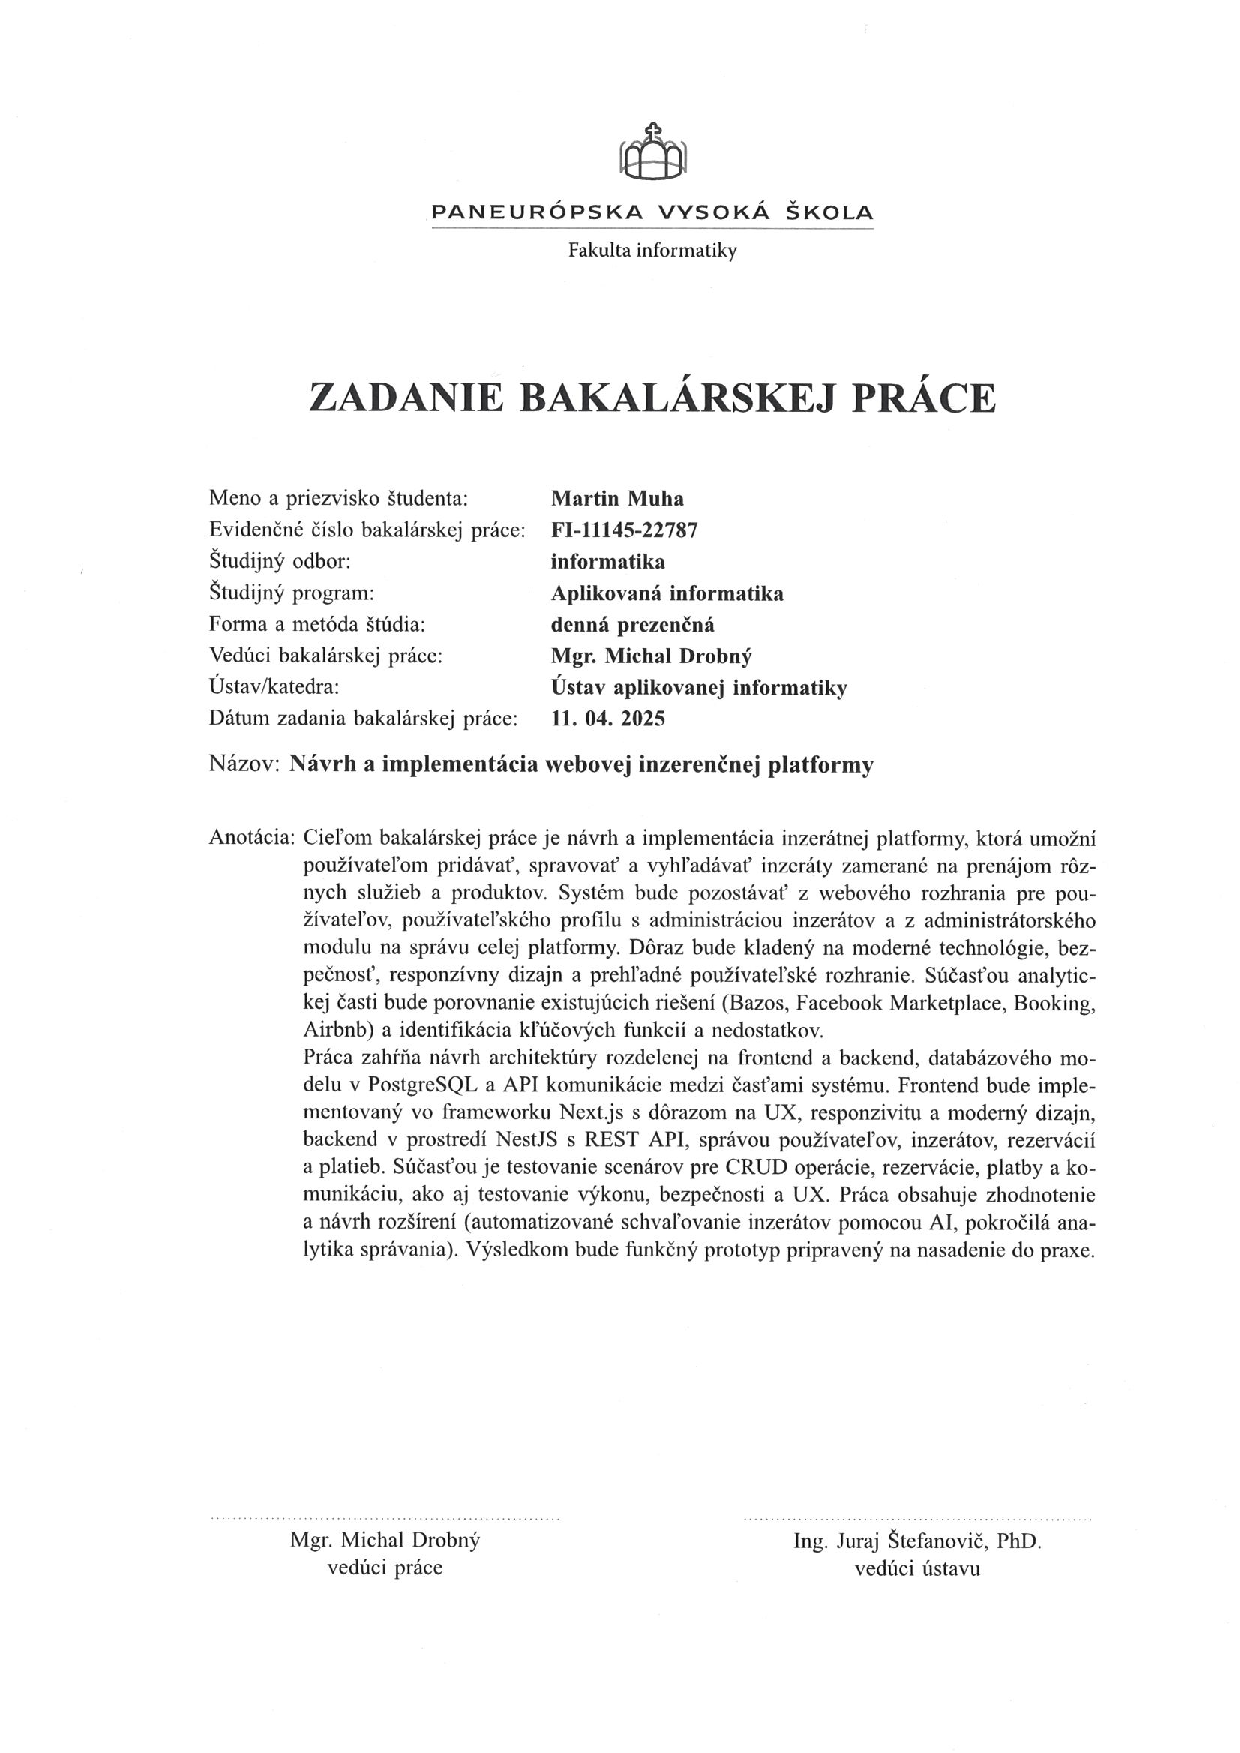
\includepdf{essentials/assignment.pdf}
%
% Poradie podľa referenčnej predlohy: Čestné vyhlásenie, potom Poďakovanie
\makeatletter
\thispagestyle{empty}
\vspace*{\fill}
\begin{flushleft}
    \textbf{Čestné vyhlásenie}\\[1em]
    \hspace*{1.5em}Čestne vyhlasujem, že som záverečnú prácu vypracoval samostatne a uviedol som všetku použitú literatúru.
\end{flushleft}
\vspace{1em}
\begin{flushright}
    \makebox[60mm][c]{\dotfill}
\end{flushright}
\clearpage
\makeatother

\makeatletter
\thispagestyle{empty}
\vspace*{\fill}
\begin{flushleft}
    \textbf{Poďakovanie}\\[1em]
    \hspace*{1.5em}Pri vypracovaní tejto bakalárskej práce by som sa rád poďakoval Mgr. Michalovi Drobnému za jeho odborné vedenie, cenné rady a konzultácie, ktoré mi významne pomohli pri spracovaní danej témy.
\end{flushleft}
\begin{flushright}
    \@author
\end{flushright}
\clearpage
\makeatother

% Abstrakt podľa referenčného formátu (ABSTRAKT + bibliografický záznam + text + kľúčové slová)
\makeatletter
\thispagestyle{empty}

\noindent\textbf{ABSTRAKT}\par\vspace{1em}

\noindent\hspace*{1.5em}\MakeUppercase{\@author{}}: \@title. \thesisHeader. Paneurópska vysoká škola. Fakulta informatiky. Školiteľ: \supervisor. Bratislava. FI PEVŠ, \thesisyear, 79~s.\par\vspace{1em}

\noindent\hspace*{1.5em}Táto práca sa zameriava na návrh a analýzu webovej aplikácie RentMe, ktorá predstavuje inovatívnu digitálnu platformu pre prenájom vecí a poskytovanie služieb v rámci jedného integrovaného systému. Aplikácia kombinuje princípy zdieľanej ekonomiky a gig ekonomiky, pričom umožňuje používateľom nielen prenajímať a vyhľadávať rôzne druhy majetku, ale zároveň ponúkať a získavať pracovné príležitosti a služby prostredníctvom inzertného systému. Cieľom aplikácie RentMe je zjednodušiť proces sprostredkovania prenájmov a služieb, zvýšiť dostupnosť lokálnych pracovných príležitostí a podporiť efektívne využívanie existujúcich zdrojov. Práca sa venuje analýze konkurenčných platforiem, návrhu funkcionalít aplikácie, technologickej architektúre a identifikácii hlavných prínosov navrhovaného riešenia. Výsledkom je koncept univerzálnej webovej platformy, ktorá prepája viacero trhových segmentov do jedného ekosystému a reaguje na aktuálne trendy digitalizácie, flexibility práce a zdieľania zdrojov.\par\vspace{1em}

\noindent\hspace*{1.5em}\textbf{Kľúčové slová:} webová aplikácia, prenájom, zdieľaná ekonomika, gig ekonomika, digitálna platforma

\clearpage
\thispagestyle{empty}

\noindent\textbf{ABSTRACT}\par\vspace{1em}

\begin{otherlanguage}{english}
\noindent\hspace*{1.5em}\MakeUppercase{\@author{}}: RentMe -- Web Platform for Advertising Services and Rental. Bachelor thesis. Pan-European University. Faculty of Informatics. Thesis supervisor: \supervisor. Bratislava. FI PEVŠ, \thesisyear, 79~p.\par\vspace{1em}

\noindent\hspace*{1.5em}This thesis focuses on the design and analysis of RentMe, a web application that represents an innovative digital platform for item rental and service provision within a single integrated system. The application combines principles of the sharing economy and gig economy, enabling users not only to rent and search for various types of assets, but also to offer and obtain employment opportunities and services through a classified advertisement system. The objective of the RentMe application is to streamline the process of mediating rentals and services, enhance the availability of local employment opportunities, and promote efficient utilization of existing resources. This work addresses the analysis of competing platforms, the design of application functionalities, technological architecture, and the identification of the main benefits of the proposed solution. The result is a concept of a universal web platform that interconnects multiple market segments into one ecosystem and responds to current trends in digitalization, work flexibility, and resource sharing.\par\vspace{1em}

\noindent\hspace*{1.5em}\textbf{Keywords:} web application, rental, sharing economy, gig economy, digital platform
\end{otherlanguage}

\clearpage
\makeatother


% Zapnúť stránkovanie pre obsah a nasledujúce sekcie (číslovanie centrované)
\pagestyle{fancy}

% ── Obsah ──────────────────────────────────────────────────────────────────
\tableofcontents
\clearpage

% ── Zoznam ilustrácií ──────────────────────────────────────────────────────
\renewcommand{\listfigurename}{Zoznam ilustrácií}
\makeatletter
% Nadpisy zoznamov: rovnaký štýl ako section (cez \listheading)
\renewcommand{\listoffigures}{%
  \listheading{\listfigurename}\@starttoc{lof}}
\renewcommand{\listoftables}{%
  \listheading{\listtablename}\@starttoc{lot}}
\makeatother
\listoffigures
\addcontentsline{toc}{section}{Zoznam ilustrácií}
\clearpage

% ── Zoznam tabuliek ────────────────────────────────────────────────────────
\listoftables
\addcontentsline{toc}{section}{Zoznam tabuliek}
\clearpage

% ── Zoznam skratiek a značiek ──────────────────────────────────────────────
\glsaddall
\addcontentsline{toc}{section}{Zoznam skratiek a značiek}
\listheading{Zoznam skratiek a značiek}
{\renewcommand{\glossarysection}[2][]{}%
 \printnoidxglossary[type=\acronymtype,title={}]}
\clearpage



%%%%%%% DOCUMENT BODY %%%%%%%
%%%%%%%%%%%%%%%%%%%%%%%%%%%%%
% Začni písať sem (prázdne od začiatku):
\section{Úvod}
\subsection{Motivácia a význam inzertných platforiem v súčasnosti}
\noindent
V súčasnej digitálnej ére prechádza spôsob, akým spotrebitelia vyhľadávajú služby a prenájmy, zásadnou transformáciou \parencite{vallas2020platforms}. Tradičné formy inzercie sú nahrádzané interaktívnymi webovými platformami, ktoré umožňujú okamžitý prístup k informáciám v reálnom čase. Hlavnou motiváciou pre vývoj modernej inzertnej platformy je potreba konsolidovať rozptýlenú ponuku do jedného transparentného a bezpečného ekosystému.

\subsubsection{Digitalizácia, dostupnosť a sieťový efekt}
Moderný používateľ očakáva vysokú mieru flexibility a rýchlosti pri hľadaní odborných služieb či prenájmu. Kľúčovým faktorom úspechu je budovanie mena aplikácie a zvyšovanie jej návštevnosti, čím vzniká takzvaný sieťový efekt~--~s rastúcim počtom inzerátov a používateľov sa zvyšuje celkový dopyt po ponukách a hodnota platformy pre celú komunitu \parencite{rochet2003platform}. Digitalizácia týchto procesov odbúrava administratívne bariéry a umožňuje efektívnejšie párovanie dopytu s ponukou.

\subsubsection{Lokalizácia a geografický kontext}
Pri službách a prenájmoch zohráva geografická poloha kritickú úlohu. Implementácia pokročilých mapových rozhraní a lokalizačných služieb (v projekte riešené cez knižnicu \hlcode{Leaflet}) umožňuje používateľom vizualizovať dostupnosť ponúk vo svojom bezprostrednom okolí \parencite{obe2017postgresql}. Tento prístup zvyšuje používateľský komfort a znižuje logistické náklady, pričom geografické vyhľadávanie sa stáva štandardom odlišujúcim profesionálne riešenia od jednoduchých textových zoznamov.

\subsubsection{Jednoduchosť a používateľská prívetivosť}
Okrem funkčnej vybavenosti je kľúčovým prvkom významu platformy jej jednoduchosť. Intuitívne používateľské rozhranie zabezpečuje, že aplikácia je prístupná širokému spektru osôb bez ohľadu na ich technické zručnosti \parencite{riva2022nextjs}. Práve nízka bariéra vstupu a rýchly proces publikácie inzerátu priamo podmieňujú ochotu používateľov opakovane sa do systému vracať. Výskumy v oblasti UX (User Experience) opakovane potvrdzujú, že každé zbytočné kliknutie alebo krok vo formulári znižuje mieru dokončenia o desiatky percent -- preto som zvolil viacstupňového sprievodcu (wizard) namiesto dlhého jednostranového formulára.

\subsubsection{Dôvera, bezpečnosť a transparentnosť}
Jednou z najväčších výziev online inzercie je eliminácia podvodného správania \parencite{hoffman2020websec}. Význam platformy spočíva v schopnosti garantovať bezpečnosť prostredníctvom aktívnej moderácie, systémov na nahlasovanie podozrivých aktivít (modul \hlcode{reports}) a prísnych pravidiel pre schvaľovanie inzerátov administrátorom. Tieto prvky, spolu s prehľadnou históriou správ, budujú nevyhnutnú dôveru medzi subjektmi v digitálnom priestore \parencite{sundararajan2014peer}.

\subsection{Definícia problému (centralizácia služieb a prenájmu)}
\noindent
Súčasný digitálny trh so službami a prenájmom na Slovensku je príliš rozdrobený, čo komplikuje kontakt medzi tými, ktorí službu ponúkajú, a tými, ktorí ju hľadajú. Hlavným problémom je chýbajúca univerzálna platforma, ktorá by dokázala spojiť rôzne profesie a typy prenájmu na jednom mieste. Používatelia sú dnes nútení hľadať riešenia cez viaceré, často špecializované alebo neformálne kanály, ktoré však nespĺňajú všetky ich potreby.

Dobrým príkladom špecializácie je portál \hlcode{pretlak.com}. Ponúka síce moderné prostredie, ale zameriava sa takmer výhradne na IT, marketing a kreatívny priemysel. Podobne sú na tom aj skupiny na sociálnych sieťach, napríklad skupina \hllink{Programátori}{https://www.facebook.com/groups/programatori/?locale=sk_SK}, ktorá slúži len úzkemu okruhu odborníkov na vývoj. Ostatné remeslá a profesie tak často končia na portáli \hlcode{bazos.sk}. Ten je však v prvom rade určený na predaj tovaru, nie na správu služieb. Navyše, jeho vizuálna stránka a ovládanie cielia skôr na staršie generácie, čo pre mladších používateľov, zvyknutých na moderné a rýchle aplikácie, predstavuje technologickú prekážku.

Ďalšou výraznou slabinou je chýbajúca štruktúra a slabé možnosti filtrovania. Na sociálnych sieťach sa príspevky radia za sebou podľa času pridania, kvôli čomu zaujímavé ponuky rýchlo zapadnú. Keďže chýba podrobné vyhľadávanie, používateľ musí manuálne prechádzať množstvo inzerátov, ktoré ho nezaujímajú. Problémom je aj chýbajúci geografický prehľad. Bez mapy a presného určenia polohy je veľmi ťažké a zdĺhavé nájsť niekoho, kto poskytuje služby priamo v okolí používateľa.

Z pohľadu bezpečnosti sú sociálne siete a fóra rizikové, pretože im chýbajú nástroje na kontrolu obsahu alebo overovanie osôb. Ak niekto poruší pravidlá, administrátor nemá k dispozícii systém, ktorý by okamžite zasiahol, čo vytvára priestor pre podvody. Prevádzkovatelia týchto skupín navyše nevedia sledovať, o čo majú ľudia skutočný záujem, pretože nemajú prístup k analytickým dátam. Moja práca na tieto nedostatky reaguje vytvorením centralizovanej platformy, ktorá spája všetky potrebné funkcie do jedného prehľadného systému s jasnými pravidlami a jednoduchým ovládaním.

\subsection{Ciele bakalárskej práce}
\noindent
Hlavným cieľom tejto bakalárskej práce je navrhnúť a vytvoriť modernú webovú platformu, ktorá slúži na uverejňovanie a správu inzerátov v oblasti služieb a prenájmu. Celý systém je navrhnutý tak, aby na jednom mieste prepojil bežných používateľov, poskytovateľov služieb a administrátorov, čím nahrádza súčasné neprehľadné hľadanie na sociálnych sieťach alebo všeobecných inzertných weboch.

Pre dosiahnutie tohto hlavného cieľa som si stanovil niekoľko konkrétnych úloh:

Prvou úlohou je vytvorenie stabilného a bezpečného technického zázemia (backendu) pomocou frameworku \hlcode{NestJS}. Tento systém musí zvládnuť bezpečnú registráciu a prihlasovanie používateľov cez \hlcode{JWT} tokeny, správne ukladať dáta do databázy \hlcode{PostgreSQL} a zabezpečiť, aby sa k citlivým údajom nedostal nikto nepovolaný. Dôležitým bodom je aj kontrola vstupných údajov, aby sa predišlo chybám alebo útokom na aplikáciu.

Druhou úlohou je vývoj troch samostatných webových aplikácií pomocou technológie \hlcode{Next.js}, ktoré sú prispôsobené konkrétnym skupinám ľudí. Verejná časť umožní návštevníkom rýchlo vyhľadávať inzeráty aj pomocou interaktívnej mapy, používateľská zóna dovolí registrovaným členom spravovať svoje ponuky a správy, a administračný panel poskytne nástroje na schvaľovanie obsahu a sledovanie štatistík. Pri tvorbe vzhľadu sa zameriavam na jednoduchosť a moderný dizajn, aby bola aplikácia príjemná pre mladšiu generáciu, no zároveň zrozumiteľná pre každého.

Posledným dôležitým cieľom je implementácia analytických nástrojov a funkcií na moderovanie obsahu. Systém bude automaticky sledovať kliknutia na inzeráty, čo správcovi pomôže pochopiť, o ktoré kategórie je najväčší záujem. Zároveň bude platforma obsahovať funkcie na nahlasovanie nevhodných inzerátov a možnosť zablokovať problémových používateľov, čím sa zvýši celková bezpečnosť a dôveryhodnosť celého systému.

\section{Súčasný stav riešenej problematiky}
\noindent
V tejto kapitole podrobujem analýze aktuálne dostupné riešenia v oblasti digitálnej inzercie a zdieľanej ekonomiky. Zameriavam sa na to, ako svetoví lídri a lokálne slovenské portály pristupujú k správe služieb a prenájmu, pričom identifikujem funkčné a technologické nedostatky, ktoré moja platforma odstraňuje.

\subsection{Analýza konkurenčných platforiem a systémov}
\noindent
Pre pochopenie štandardov v odvetví je nevyhnutné analyzovať systémy, ktoré definujú súčasné trendy v oblasti digitálnych trhovísk (marketplace). Tieto platformy reprezentujú rôzne logické prístupy k spracovaniu dát a budovaniu dôvery medzi používateľmi \parencite{rochet2003platform}. Na základe analýzy identifikujem ich silné stránky, ktoré som do vlastného riešenia prevzal, a zároveň ich obmedzenia, ktoré moja platforma prekonáva.

\subsubsection[Airbnb.com]{Airbnb.com (Model zdieľanej ekonomiky ubytovania)}
\textbf{Charakteristika a logika:} Airbnb je prototypom modernej P2P platformy, ktorá zmenila celé odvetvie ubytovania. Platforma funguje ako dôveryhodný sprostredkovateľ medzi súkromnými prenajímateľmi a hosťami, pričom kľúčovú rolu hrá obojstranný systém hodnotení a overovanie identity \parencite{sundararajan2014peer}.

\textbf{Výhody:} Sofistikovaný reputačný systém, geografické vyhľadávanie s mapovým rozhraním a dynamické ceny na základe dopytu a sezónnosti.

\textbf{Nevýhody:} Platforma je úzko špecializovaná na krátkodobý prenájom ubytovania. Vysoké poplatky pre hostiteľov (15–20\,\% z každej rezervácie) odrádzajú malých lokálnych prenajímateľov. Model tiež predpokladá štandardizovateľnosť ponuky, čo je pri remeslách a službách ťažko dosiahnuteľné.

\textbf{Porovnanie s vlastným riešením:} Z Airbnb preberám kľúčovú filozofiu: technológia musí prekonať nedôveru medzi cudzími ľuďmi. V mojom riešení je to realizované cez moderáciu inzerátov, systém nahlásení (\hlcode{Reports}) a jasnú identitu každého inzerenta. Na rozdiel od Airbnb moja platforma neúčtuje provízie -- monetizačný model je postavený na prémiových plánoch inzerentov (\hlcode{SellerPlan}).

\subsubsection[OLX/Bazoš]{OLX / Bazoš.sk (Model všeobecnej inzercie)}
\textbf{Charakteristika a logika:} OLX (pôsobí v strednej a východnej Európe) a jeho slovenský ekvivalent Bazoš.sk sú najrozšírenejšími platformami pre všeobecnú inzerciu v regióne. Modely sú postavené na maxime dosahu -- veľký počet inzerátov, minimálne prekážky pre pridanie ponuky \parencite{vallas2020platforms}.

\textbf{Výhody:} Vysoká návštevnosť a povedomie značky. Jednoduché pridanie inzerátu bez registrácie. Pokrytie širokého spektra kategórií od elektroniky po nehnuteľnosti.

\textbf{Nevýhody:} Absencia moderácie vedie k množstvu neaktuálnych, duplicitných alebo podvodných inzerátov. Platforma nemá natívny chat ani systém správ -- komunikácia prebieha cez zverejnené telefónne číslo, čo narúša súkromie a neumožňuje sledovanie konverzácií. Chýba geografická vizualizácia (mapa) a pokročilé filtrovanie. Vizuálne zastarané rozhranie necieli na mladšiu generáciu.

\textbf{Porovnanie s vlastným riešením:} Moja platforma rieši každý zo zmienených nedostatkov: povinná moderácia zabezpečuje kvalitu obsahu, integrovaný chat chráni súkromie používateľov a Leaflet mapa s GPS filtráciou umožňuje presné geografické vyhľadávanie.

\subsubsection[Booking.com]{Booking.com (Model komplexnej rezervácie a správy kapacít)}
\textbf{Charakteristika a logika:} Booking.com operuje na báze pokročilých algoritmov pre správu voľných kapacít v reálnom čase \parencite{rochet2003platform}. Systém je postavený na okamžitej potvrdenej rezervácii a dynamickej tvorbe cien, čo si vyžaduje robustnú architektúru na zamedzenie duplicitných rezervácií.

\textbf{Výhody:} Extrémne podrobné hierarchické filtrovanie a vysoká miera dôveryhodnosti budovaná cez overené recenzie.

\textbf{Nevýhody:} Systém je uzavretý výhradne pre segment ubytovania. Pre malých lokálnych poskytovateľov iných služieb sú prekážkou vysoké provízie a rigidita systému, ktorý neumožňuje inzerovať predmety dennej potreby alebo remeselné práce.

\textbf{Porovnanie s vlastným riešením:} Moja platforma preberá logiku podrobného filtrovania meta-údajov, avšak aplikuje ju univerzálne. Vďaka flexibilnej schéme v \hlcode{Prisma ORM} umožňujem inzerátom priraďovať rôzne špecifikácie (napr. technické parametre náradia) bez nutnosti meniť základnú architektúru databázy.

\subsubsection[Fiverr.com]{Fiverr.com (Model produktizácie služieb -- Micro-gig economy)}
\textbf{Charakteristika a logika:} Fiverr transformoval nehmotné služby na jasne definované balíčky (produkty) \parencite{vallas2020platforms}. Logika fungovania spočíva v eliminácii vyjednávania o cene a rozsahu práce, čím sa proces nákupu služby približuje klasickému elektronickému obchodu.

\textbf{Výhody:} Prehľadnosť nákupného procesu a automatizované filtrovanie kvality poskytovateľov cez systém úrovní.

\textbf{Nevýhody:} Orientácia takmer výhradne na digitálne produkty doručiteľné online. Absencia lokalizačnej vrstvy a máp znemožňuje efektívne sprostredkovanie fyzických služieb v konkrétnom meste.

\textbf{Porovnanie s vlastným riešením:} Implementujem logiku „služba ako produkt“, ale obohacujem ju o kľúčový geografický kontext. Integrácia mapových podkladov cez knižnicu \hlcode{Leaflet} a ukladanie GPS súradníc v \hlcode{PostgreSQL} umožňuje používateľom nájsť odborníka v ich bezprostrednom okolí.

\subsubsection[Turo.com]{Turo.com (Model Peer-to-Peer zdieľania majetku)}
\textbf{Charakteristika a logika:} Turo reprezentuje model zdieľanej ekonomiky v doprave, kde súkromné osoby monetizujú svoj nevyužitý majetok (automobily) \parencite{sundararajan2014peer}. Logika systému stojí na overovaní identity a synchronizácii s kalendárom vlastníka.

\textbf{Výhody:} Efektívne využitie existujúcich zdrojov a prepracovaná vizuálna prezentácia majetku.

\textbf{Nevýhody:} Ide o jednoúčelovú aplikáciu. Ak používateľ hľadá iný typ prenájmu (napr. stavebnú techniku), je nútený využiť ďalší samostatný systém.

\textbf{Porovnanie s vlastným riešením:} Navrhované riešenie predstavuje integrovaný ekosystém, ktorý konsoliduje fragmentované potreby lokálneho trhu do jedinej platformy, čím odstraňuje nutnosť využívania viacerých jednoúčelových aplikácií.

\subsection{Ekonomické modely modernej inzercie}
\noindent
Pre pochopenie fungovania navrhovanej platformy je nevyhnutné definovať kľúčové ekonomické koncepty, ktoré v poslednom desaťročí transformovali globálny trh práce a služieb. Podľa správy Európskej komisie z roku 2021 sa obrat platforiem zdieľanej ekonomiky v EÚ od roku 2015 strojnásobil a v roku 2020 presiahol 60 miliárd eur, pričom segment služieb a prenájmu rastie najrýchlejšie \parencite{vallas2020platforms}.

\subsubsection{Fenomén Micro-gig economy}
Micro-gig economy (často označovaná aj ako „platformová ekonomika”) predstavuje model, v ktorom sú dlhodobé pracovné pomery nahrádzané krátkodobými, presne definovanými úlohami, takzvanými „gigmi”. Tento model zmenil vnímanie práce z fixného zamestnania na poskytovanie konkrétnej hodnoty v reálnom čase \parencite{vallas2020platforms}. Podľa odhadov Medzinárodnej organizácie práce (ILO) sa počet pracovníkov zapojených do platformovej ekonomiky celosvetovo medzi rokmi 2013 a 2020 zdvojnásobil.

\textbf{Logika a fungovanie:} Základom je digitalizácia dopytu. Platforma funguje ako algoritmus, ktorý páruje voľné kapacity dodávateľa s okamžitou potrebou odberateľa \parencite{rochet2003platform}. Na rozdiel od klasickej inzercie sa tu hľadá „riešenie problému”. Príkladom je platforma Fiverr, kde je služba predávaná ako vopred zabalený produkt s fixnou cenou a termínom dodania. Tento prístup eliminuje transakčné náklady spojené s vyjednávaním a zmluvnou dokumentáciou.

\textbf{Výhody pre trh:} Tento model umožňuje obrovskú mieru flexibility. Freelanceri môžu pracovať pre viacerých klientov súčasne a záujemcovia majú prístup k expertom bez nutnosti uzatvárania zložitých zmlúv. Pre lokálne trhy ako Slovensko je osobitne dôležitá možnosť, že aj malý remeselník dokáže osloviť zákazníkov v celom regióne bez investície do vlastného marketingu.

\textbf{Riziká a výzvy:} Gig economy čelí aj kritike -- nedostatočná právna ochrana pracovníkov, nestabilný príjem a závislosť na algoritmickom hodnotení sú legitímne obavy \parencite{vallas2020platforms}. Moja platforma tieto riziká adresuje tým, že nepreberie rolu zamestnávateľa, ale zostáva neutrálnym sprostredkovateľom, ktorý dáva inzerentom plnú kontrolu nad podmienkami a cenou.

\textbf{Aplikácia v mojom projekte:} Moja platforma preberá z tohto modelu princíp „produktizácie” služieb. Vytvoril som systém, kde si používateľ nevyberá len osobu, ale konkrétnu ponuku s jasnými parametrami. Vďaka modulu \hlcode{Advertisements} a dynamickým filtrom umožňujem inzerentom presne definovať rozsah svojej „mikro-zákazky” -- vrátane ceny, lokality a technických špecifikácií -- čím znižujem čas potrebný na vyjednávanie a zvyšujem transparentnosť transakcie.

\subsubsection{Model Peer-to-Peer (P2P) a zdieľaná ekonomika}
Model Peer-to-Peer (rovný s rovným) je základným stavebným kameňom zdieľanej ekonomiky. Ide o transakcie, ktoré prebiehajú priamo medzi dvoma koncovými používateľmi, pričom platforma vystupuje len ako technologický sprostredkovateľ a garant bezpečnosti \parencite{sundararajan2014peer}.

\textbf{Logika zdieľania majetku:} Hlavnou myšlienkou je efektívna monetizácia nevyužitých statkov \parencite{sundararajan2014peer}. V praxi to znamená, že osoba, ktorá vlastní napríklad rebríkový záves, elektrické náradie či pracovné stroje, môže tieto aktíva prenajímať susedovi namiesto toho, aby ležali nevyužité. Tento prístup je nielen ekonomicky výhodný pre obe strany, ale aj ekologicky udržateľný -- znižuje potrebu výroby nových výrobkov. Platformy ako Airbnb dokázali, že technológia dokáže prekonať prirodzenú nedôveru medzi cudzími ľuďmi a vybudovať fungujúce trhovisko na báze reputácie.

\textbf{Budovanie dôvery -- kľúčový problém P2P:} Kľúčovým prvkom P2P logiky je reputačný systém a moderácia \parencite{rochet2003platform}. Bez možnosti nahlásiť nekorektné správanie, overiť totožnosť inzerenta alebo ohodnotiť transakciu by tento model skolaboval -- potenciálnych záujemcov by odradila neistota. Štúdie ukazujú, že platformy s aktívnou moderáciou a systémom hodnotení dosahujú o 30–40\,\% vyššiu mieru opakovaného použitia \parencite{sundararajan2014peer}.

\textbf{Aplikácia v mojom projekte:} Moja platforma je postavená na P2P princípe najmä v segmente prenájmu. Implementoval som moduly \hlcode{Messages} pre bezpečnú komunikáciu (používateľ nemusí zverejniť svoje telefónne číslo a komunikácia môže prebehnúť výhradne cez integrovaný chat), \hlcode{Reports} pre nahlasovanie incidentov a systém moderácie, ktorý zaručuje, že na platforme sa objavia len overené inzeráty. Na rozdiel od platforiem ako Bazoš.sk môj systém vďaka administrátorskému panelu umožňuje aktívne zasahovať, sledovať trendové kategórie a chrániť používateľov v reálnom čase.

\subsubsection{Slovenský trh a lokálna príležitosť}
\noindent
Slovenský trh digitálnych služieb a prenájmu vykazuje špecifické charakteristiky, ktoré vytvárajú priestor pre lokálne riešenie. Dominantné platformy ako Bazoš.sk slúžia primárne predaju tovaru, nie sprostredkovaniu služieb a prenájmu. Portál pretlak.com pokrýva len kreatívne a IT profesie. Výsledkom je, že desiatky tisíc remeselníkov, živnostníkov a malých poskytovateľov služieb nemajú k dispozícii modernú digitálnu vitrínu, ktorá by zodpovedala ich potrebám \parencite{vallas2020platforms}.

Tento „biely priestor” na trhu predstavuje hlavnú podnikateľskú príležitosť navrhovanej platformy RentMe. Cieľom nie je konkurovať globálnym gigantom, ale obsadiť lokálny segment, kde veľkí hráči nie sú prítomní alebo kde ich riešenia nie sú prispôsobené lokálnym zvyklostiam, jazyku a právnemu prostrediu.

\subsection{Technologické trendy a pridaná hodnota riešenia}
\noindent
Aby aplikácia obstála v konkurencii, využíva moderný technologický stack, ktorý rieši slabiny starších portálov. Volba technológií nie je len technické rozhodnutie -- priamo ovplyvňuje rýchlosť vývoja, bezpečnosť systému a dlhodobú udržateľnosť kódu \parencite{winters2020swe}.

\textbf{Server-side Rendering (\hlcode{Next.js}):} Zabezpečuje rýchle načítanie a lepšiu indexáciu inzerátov vyhľadávačmi (SEO), čo je kľúčové pre návštevnosť verejnej platformy \parencite{riva2022nextjs}.

\textbf{Typová bezpečnosť (\hlcode{TypeScript}):} Použitie monorepa umožňuje zdieľať dátové modely (DTO) medzi API a frontend aplikáciami, čím sa minimalizuje riziko nekonzistencií v dátach \parencite{cherny2019typescript}.

\textbf{Analytika (\hlcode{ClickEvent}):} Na rozdiel od neformálnych riešení (Facebook skupiny) systém monitoruje správanie používateľov (kliknutia, segmentácia podľa pohlavia či typu účtu), čo umožňuje administrátorovi optimalizovať kategórie podľa skutočného dopytu \parencite{winters2020swe}.

\section{Analýza a návrh systému}
\noindent
Návrh systému vychádza z rozdelenia platformy na štyri základné časti: verejná platforma, používateľské konto, admin panel a backend API \parencite{sommerville2015se}. Tento prístup, realizovaný pomocou monorepo štruktúry a oddelených \hlcode{Next.js} aplikácií, umožňuje presne definovať oprávnenia pre rôzne skupiny používateľov a izolovať ich používateľské rozhrania.

\subsection{Funkčné požiadavky}
\noindent
Funkčné požiadavky sú rozdelené podľa rolí, ktoré v systéme vystupujú \parencite{sommerville2015se}. Každá rola má priradený špecifický rozsah akcií, ktoré môže v rámci aplikácie vykonávať. Na úrovni databázy je rola používateľa definovaná enumerátorom \hlcode{UserRole} (s hodnotami \hlcode{ADMIN} a \hlcode{USER}).

Obrázok~\ref{fig:usecase-funkcne} zobrazuje diagram použitia (Use Case): vzťahy medzi aktérmi (Návštevník, Používateľ, Administrátor) a vybranými prípadmi použitia. Pri aktérovi Používateľ je šípkou zovšeobecnenia (UML generalization) znázornené, že okrem vlastných prípadov použitia zdedí aj možnosti návštevníka.

\begin{figure}[htbp]
\centering
\resizebox{\textwidth}{!}{% Diagram použitia (Use Case) — funkčné požiadavky (sekcia 3.1)
% Vizuál: UML panáci, jemné tiene, ortogonálne asociácie
\begin{tikzpicture}[
  font=\sffamily\small,
  >=Stealth,
  line cap=round,
  line join=round,
  % Karta aktéra (UML štýl)
  actorcard/.style={
    rectangle,
    rounded corners=5pt,
    minimum width=1.85cm,
    minimum height=2.05cm,
    inner sep=5pt,
    align=center,
    fill=blue!3!white,
    draw=blue!28!black!35,
    line width=0.45pt
  },
  % Prípad použitia
  usecase/.style={
    ellipse,
    draw=teal!45!black!80,
    line width=0.55pt,
    fill=white,
    minimum width=3.05cm,
    minimum height=1.05cm,
    align=center,
    inner sep=4pt,
    drop shadow={
      shadow xshift=0.35pt,
      shadow yshift=-0.85pt,
      opacity=0.14,
      fill=black
    }
  },
  % Asociácia aktér–prípad (UML: plná čiara, bez šípky)
  assoc/.style={
    draw=black!35,
    line width=0.7pt,
    rounded corners=2pt
  },
  % Zovšeobecnenie medzi aktérmi
  gen/.style={
    draw=black!48,
    line width=0.75pt,
    -{Triangle[open, length=4.2mm, width=5mm]}
  }
]

% --- Panák (opakovateľná kresba cez scope posun)
\newcommand{\umlstick}{%
  \begin{scope}[line width=0.68pt, draw=black!68]
    \draw (0,0.56) circle (0.135);
    \draw (0,0.425) -- (0,-0.06);
    \draw (-0.2,0.17) -- (0.2,0.17);
    \draw (0,-0.06) -- (-0.16,-0.44);
    \draw (0,-0.06) -- (0.16,-0.44);
  \end{scope}%
}

% --- Aktéri
\node[actorcard] (A1) at (-2.45, 6.35) {%
  \begin{tikzpicture}[baseline=-0.58cm]
    \umlstick
  \end{tikzpicture}\\[-1pt]
  {\footnotesize\bfseries\sffamily\color{black!80} Návštevník}
};
\node[actorcard] (A2) at (-2.45, 3.55) {%
  \begin{tikzpicture}[baseline=-0.58cm]
    \umlstick
  \end{tikzpicture}\\[-1pt]
  {\footnotesize\bfseries\sffamily\color{black!80} Používateľ}
};
\node[actorcard] (A3) at (-2.45, 0.35) {%
  \begin{tikzpicture}[baseline=-0.58cm]
    \umlstick
  \end{tikzpicture}\\[-1pt]
  {\footnotesize\bfseries\sffamily\color{black!80} Administrátor}
};

% Zovšeobecnenie Používateľ → Návštevník
\draw[gen] (A2.north) -- (A1.south);

% --- Prípady použitia (mriežka)
\node[usecase] (U1) at (2.15, 6.55) {Prehliadať\\[-1pt]inzeráty};
\node[usecase] (U2) at (2.15, 4.45) {Hľadať na\\[-1pt]mape};
\node[usecase] (U3) at (2.15, 2.35) {Registrovať sa};

\node[usecase] (U4) at (7.05, 6.55) {Pridať\\[-1pt]inzerát};
\node[usecase] (U5) at (7.05, 4.45) {Poslať správu};
\node[usecase] (U6) at (7.05, 2.35) {Spravovať\\[-1pt]profil};

\node[usecase] (U7) at (4.55, 0.55) {Schvaľovať\\[-1pt]inzeráty};
\node[usecase] (U8) at (4.55, -1.05) {Banovať\\[-1pt]používateľov};
\node[usecase] (U9) at (4.55, -2.65) {Spravovať\\[-1pt]kategórie};

% Hranica systému
\begin{scope}[on background layer]
  \node[
    fill=blue!1!gray!2,
    draw=blue!32!black!45,
    line width=0.85pt,
    dashed,
    dash pattern=on 4.2pt off 3.4pt,
    rounded corners=8pt,
    inner sep=20pt,
    fit=(U1)(U2)(U3)(U4)(U5)(U6)(U7)(U8)(U9),
    label={[yshift=4pt, text=black!72]above:{\bfseries\sffamily\normalsize Systém inzertnej platformy}}
  ] {};
\end{scope}

% Ortogonálne asociácie (predĺženie z pravého okraja karty)
\newcommand{\actorOut}[2]{($(#1.east)+(0.12,0)$) -- ++(0.28,0) |- (#2.west)}
\draw[assoc] \actorOut{A1}{U1};
\draw[assoc] \actorOut{A1}{U2};
\draw[assoc] \actorOut{A1}{U3};

\draw[assoc] \actorOut{A2}{U4};
\draw[assoc] \actorOut{A2}{U5};
\draw[assoc] \actorOut{A2}{U6};

\draw[assoc] \actorOut{A3}{U7};
\draw[assoc] \actorOut{A3}{U8};
\draw[assoc] \actorOut{A3}{U9};

\end{tikzpicture}
}
\caption{Diagram použitia (Use Case) -- funkčné požiadavky a aktéri systému}
\label{fig:usecase-funkcne}
\end{figure}

\subsubsection[Návštevník]{Rola: Návštevník (neprihlásený používateľ)}
\noindent
Návštevník je anonymný používateľ, ktorý primárne konzumuje verejne dostupný obsah bez potreby registrácie.

\begin{itemize}
  \item \textbf{Prehliadanie obsahu:} Používateľ môže prehliadať kategórie, zoznamy inzerátov a detaily jednotlivých ponúk.
  \item \textbf{Vyhľadávanie a filtrácia:} Možnosť vyhľadávať inzeráty podľa kľúčových slov a filtrovať výsledky na základe dynamických parametrov kategórie.
  \item \textbf{Mapové zobrazenie:} Prístup k interaktívnej mape, ktorá vizualizuje polohu inzerovaných služieb a prenájmov.
  \item \textbf{Čítanie blogu:} Možnosť čítať publikované články a statické informačné stránky (napr. podmienky používania).
  \item \textbf{Registrácia:} Návštevník má možnosť vytvoriť si používateľský účet.
\end{itemize}

\subsubsection[Používateľ]{Rola: Používateľ (registrovaný člen)}
\noindent
Používateľ má po prihlásení prístup k funkciám, ktoré umožňujú aktívnu participáciu na trhu služieb. Prístup k týmto funkciám je na backende chránený pomocou JWT autentifikácie (v \hlcode{NestJS} implementovanej cez \hlcode{JwtAuthGuard}).

\begin{itemize}
  \item \textbf{Správa profilu:} Úprava osobných údajov, firemných údajov (napr. IČO, DIČ) a zmena prístupového hesla.
  \item \textbf{Manažment inzerátov:} Tvorba nových inzerátov (služba alebo prenájom), ich úprava, mazanie a sledovanie stavu schválenia. V databáze môže inzerát nadobúdať stavy definované enumerátorom \hlcode{AdvertisementStatus} (\hlcode{PENDING}, \hlcode{DRAFT}, \hlcode{ACTIVE}, \hlcode{INACTIVE}, \hlcode{ARCHIVED}).
  \item \textbf{Komunikačný modul:} Odosielanie a prijímanie správ (dopytov) k inzerátom prostredníctvom integrovaného chatu.
  \item \textbf{Obľúbené položky:} Ukladanie zaujímavých inzerátov do vlastného zoznamu pre neskorší návrat (entita \hlcode{Favorite}).
  \item \textbf{Nahlasovanie (Reportovanie):} Možnosť nahlásiť inzerát, ktorý porušuje pravidlá platformy.
\end{itemize}

\subsubsection[Administrátor]{Rola: Administrátor}
\noindent
Administrátor má najvyššiu úroveň oprávnení a dohliada na technický a obsahový chod platformy cez dedikovaný admin panel. Na úrovni API sú tieto endpointy chránené kombináciou \hlcode{JwtAuthGuard} a vlastného \hlcode{RolesGuard}, ktorý overuje, či má prihlásený používateľ rolu \hlcode{ADMIN}.

\noindent
\noindent\begin{minipage}{\linewidth}% výpis v minipage sa nerozdelí naprieč stranami
\begin{lstlisting}[language=Java]
@Controller('admin')
@UseGuards(JwtAuthGuard, RolesGuard)
@Roles(UserRole.ADMIN)
export class AdminController {
  // ...
  @Get('stats')
  getStats() {
    return this.adminService.getStats();
  }
}
\end{lstlisting}
\end{minipage}
\vspace{0.4\baselineskip}
\begingroup
\captionsetup{justification=centering, singlelinecheck=false}
\captionof{lstlisting}{Ukážka zabezpečenia administrátorského endpointu v NestJS.}
\label{lst:admin-endpoint}
\endgroup

\begin{itemize}
  \item \textbf{Moderácia obsahu:} Schvaľovanie, zamietanie alebo archivácia inzerátov a riešenie prijatých nahlásení od používateľov.
  \item \textbf{Správa používateľov:} Prehľad o registrovaných členoch s možnosťou udelenia dočasného alebo trvalého banu (blokovania účtu). Databázový model \hlcode{User} obsahuje na tento účel polia \hlcode{banned}, \hlcode{bannedUntil} a \hlcode{banReason}.
  \item \textbf{CMS (Content Management System):} Tvorba a editácia statických stránok, blogových príspevkov a správa položiek v navigačnom menu.
  \item \textbf{Konfigurácia systému:} Nastavovanie kategórií, hierarchie filtrov a globálnych parametrov platformy.
  \item \textbf{Analytika a prehľady:} Sledovanie štatistík návštevnosti, kliknutí (\hlcode{ClickEvent}) a trendov v inzercii prostredníctvom grafov.
\end{itemize}

\subsection{Nefunkčné požiadavky}
\noindent
Nefunkčné požiadavky definujú technické limity a prevádzkové vlastnosti, ktoré sú nevyhnutné pre spoľahlivý chod platformy \parencite{sommerville2015se}. Pri systéme, ktorý sprostredkováva interakciu medzi cudzími ľuďmi a narába s ich citlivými údajmi, som kládol dôraz predovšetkým na bezpečnosť, jednoduchú rozšíriteľnosť a rýchlu odozvu používateľského rozhrania.

\subsubsection[Bezpečnosť]{Bezpečnosť a ochrana údajov}
\noindent
Vzhľadom na to, že platforma spracováva používateľské profily a súkromnú komunikáciu, je bezpečnosť prioritou.

\textbf{Autentifikácia a autorizácia:} Prístup k citlivým častiam API je chránený platným JSON Web Tokenom (JWT). V prostredí \hlcode{NestJS} je táto vrstva realizovaná pomocou stratégie \hlcode{passport-jwt} a chránená globálnymi guardmi (\hlcode{JwtAuthGuard}, \hlcode{RolesGuard}), ktoré pri každej požiadavke overujú identitu aj priradenú rolu používateľa.

\textbf{Hashovanie hesiel:} Heslá nie sú v databáze \hlcode{PostgreSQL} nikdy ukladané v čitateľnej podobe. Na ich bezpečnú transformáciu využívam kryptografický algoritmus \hlcode{bcrypt} so soľou (salt), čo znemožňuje ich spätné dešifrovanie.

\textbf{Validácia vstupov:} Aby som predišiel útokom typu \emph{mass assignment} alebo spracovaniu neúplných dát, systém automaticky filtruje každú prichádzajúcu požiadavku pomocou globálneho \hlcode{ValidationPipe}. Tento nástroj pracuje v spolupráci s knižnicou \hlcode{class-validator} a DTO triedami -- polia, ktoré nie sú v DTO definované, sú automaticky odmietnuté. Toto opatrenie bráni scenáru, pri ktorom by útočník poslal nepovolené polia (napr. \hlcode{role:\,"ADMIN"}) s cieľom zmeniť citlivé atribúty objektu.

\textbf{CORS a blokovanie zneužitia:} API má presne definované povolené zdroje (origins), čím sa bráni neautorizovaným volaniam z cudzích domén. Zároveň systém obsahuje mechanizmus banovania, ktorý administrátorovi umožňuje okamžite zablokovať prístup nahláseným používateľom (využitím polí \hlcode{banned} a \hlcode{banReason} v databáze).

\subsubsection[Škálovateľnosť]{Škálovateľnosť a udržateľnosť systému}
\noindent
Platforma je navrhnutá tak, aby bolo možné v budúcnosti jednoducho pridávať nové funkcie bez nutnosti prepisovania existujúceho kódu.

\textbf{Architektúra monorepa:} Využitie \hlcode{npm workspaces} mi umožnilo logicky oddeliť frontendové aplikácie (\hlcode{platform}, \hlcode{user}, \hlcode{admin}) od backendu (\hlcode{api}). Vďaka zdieľanému balíku \hlcode{packages/shared} sú dátové typy a DTO konzistentné naprieč celým projektom, čo výrazne znižuje chybovosť pri vývoji.

\textbf{Modularita a ORM:} Backend je rozdelený do samostatných doménových modulov (napr. \hlcode{AuthModule}, \hlcamel{Advertisements}{Module}), čo uľahčuje údržbu a testovanie. Použitie \hlcode{Prisma ORM} zasa zabezpečuje, že zmeny v dátovom modeli sú typovo bezpečné a ľahko nasaditeľné pomocou verziovaných migrácií.

\textbf{Kontajnerizácia:} Celý projekt je pripravený na nasadenie cez Docker. Súbor \hlcode{docker-compose.yml} definuje izolované prostredia pre databázu aj Node.js služby, čo zaručuje, že aplikácia sa bude správať identicky na mojom počítači aj na produkčnom serveri.

\subsubsection[Výkon]{Výkon, odozva a SEO}
\noindent
Rýchlosť načítania a viditeľnosť vo vyhľadávačoch sú kľúčové pre úspech každého inzertného portálu.

\textbf{Server-side Rendering (SSR):} Vďaka \hlcode{Next.js} (verzia 16+) sa obsah inzerátov generuje priamo na serveri. To zabezpečuje nielen okamžitú odozvu pre používateľa, ale aj ideálnu indexáciu Google robotmi, keďže HTML dokument už pri načítaní obsahuje dôležité SEO metadáta.

\textbf{Optimalizácia databázy:} Pre zrýchlenie vyhľadávania pri veľkom množstve dát som v Prisma schéme definoval indexy (\hlcode{@@index}) pre najčastejšie filtrované polia, ako sú \hlcode{status}, \hlcode{userId}, \hlcode{categoryId} a \hlcode{createdAt}.

\textbf{Responzívny dizajn:} Používateľské rozhranie postavené na \hlcode{Tailwind CSS} využíva prístup mobile-first. To zaručuje, že platforma je plne funkčná a vizuálne príťažlivá na smartfónoch aj veľkých monitoroch.

\textbf{Práca s médiami:} API je optimalizované na spracovanie väčších objemov dát (limit 50\,MB), čo umožňuje bezproblémový prenos obrázkov inzerátov kódovaných vo formáte \hlcode{base64}.

\subsection[Návrh architektúry]{Návrh architektúry: Model klient\,--\,server v prostredí monorepa}
\noindent
Architektúra systému je postavená na modernom koncepte monorepa, ktorý umožňuje efektívnu správu viacerých samostatných aplikácií a zdieľaných knižníc v rámci jedného úložiska (repozitára) \parencite{winters2020swe}. Celý ekosystém je rozdelený na klientske aplikácie (front-end) a centrálny server (back-end), ktoré medzi sebou komunikujú prostredníctvom protokolu HTTP a formátu JSON.

\subsubsection[Štruktúra monorepa]{Štruktúra monorepa a zdieľanie kódu}
\noindent
Projekt využíva nástroj \hlcode{npm workspaces}, ktorý zabezpečuje logické rozdelenie kódu do dvoch hlavných kategórií: aplikácie (\hlcode{apps/}) a balíčky (\hlcode{packages/}).

\begin{itemize}
  \item \textbf{Aplikácie (\hlcode{apps/}):} Obsahujú tri nezávislé \hlcode{Next.js} aplikácie s App Routerom (verzia 16+): verejnú platformu (\hlcode{apps/platform}), používateľské konto (\hlcode{apps/user}) a administráciu (\hlcode{apps/admin}). Štvrtou aplikáciou je centrálny \hlcode{NestJS} API server (\hlcode{apps/api}).
  \item \textbf{Zdieľané balíčky (\hlcode{packages/}):} Kľúčovým prvkom je balík \hlcode{packages/shared}, ktorý obsahuje spoločné TypeScript typy, enumerátory (napríklad \hlcode{UserRole} a \hlcode{AdvertisementStatus}) a objekty DTO (Data Transfer Objects). Vďaka tomu je zaručené, že ak sa zmení štruktúra dát na backende, zmena sa okamžite premietne aj do frontendu, čím sa predchádza nekonzistenciám a chybám pri kompilácii.
  \item \textbf{Databázový balík:} Balík \hlcode{packages/database} obsahuje definíciu Prisma schémy (\hlcode{schema.prisma}), vygenerovaného Prisma klienta a migračné skripty. Týmto je prístup k databáze centralizovaný a zdieľaný pre potreby API.
\end{itemize}

\subsubsection[Model klient--server]{Model klient--server}
\noindent
Systém funguje na princípe striktného oddelenia prezentácie od aplikačnej logiky a ukladania dát. Celkový pohľad na komponentovú architektúru -- vrátane troch nezávislých frontendov, centrálneho API, perzistenčnej vrstvy a zdieľaných npm balíkov -- zobrazuje obrázok~\ref{fig:architecture}.

\begin{figure}[htbp]
\centering
\resizebox{\textwidth}{!}{% Komponentová architektúra systému RentMe (portrait)
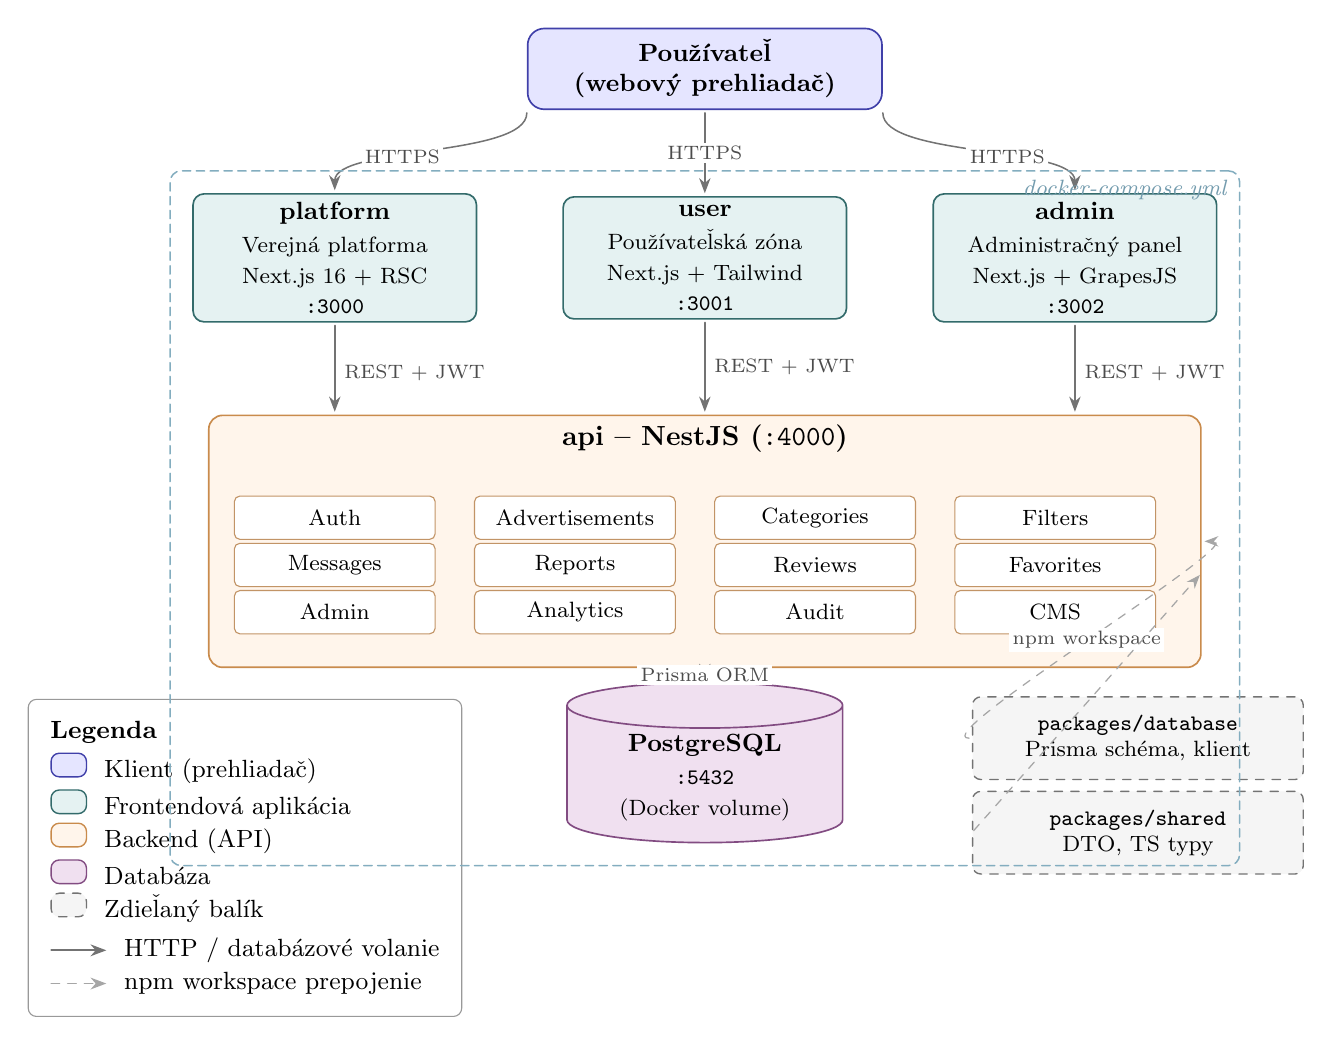
\begin{tikzpicture}[
  font=\rmfamily\small,
  line cap=round, line join=round,
  >=Stealth,
  node distance=0.6cm and 0.5cm,
  % Klient (prehliadač) — modrý
  client/.style={
    rectangle, rounded corners=6pt,
    minimum width=4.5cm, minimum height=1.0cm,
    align=center, inner sep=4pt,
    line width=0.6pt,
    draw=blue!55!black!75, fill=blue!10!white,
    font=\rmfamily\bfseries\small
  },
  % Frontendy — zelené
  frontend/.style={
    rectangle, rounded corners=4pt,
    minimum width=3.6cm, minimum height=1.55cm,
    align=center, inner sep=3pt,
    line width=0.6pt,
    draw=teal!55!black!80, fill=teal!10!white,
    font=\rmfamily\small
  },
  % Backend — oranžový
  backend/.style={
    rectangle, rounded corners=5pt,
    minimum width=12.6cm, minimum height=3.2cm,
    align=center, inner sep=4pt,
    line width=0.6pt,
    draw=orange!70!black!70, fill=orange!8!white
  },
  modulebox/.style={
    rectangle, rounded corners=2pt,
    minimum width=2.55cm, minimum height=0.55cm,
    align=center, inner sep=2pt,
    line width=0.4pt,
    draw=orange!60!black!60, fill=white,
    font=\rmfamily\footnotesize
  },
  % DB — fialová
  database/.style={
    cylinder, shape border rotate=90,
    aspect=0.25,
    minimum width=3.5cm, minimum height=1.4cm,
    align=center, inner sep=2pt,
    line width=0.6pt,
    draw=violet!60!black!70, fill=violet!12!white,
    font=\rmfamily\small
  },
  % Zdieľané balíky — sivé
  pkgbox/.style={
    rectangle, rounded corners=3pt,
    minimum width=4.2cm, minimum height=1.05cm,
    align=center, inner sep=3pt,
    line width=0.5pt, dashed,
    draw=black!55, fill=gray!8!white,
    font=\rmfamily\footnotesize
  },
  % Šípky
  arr/.style={->, line width=0.55pt, draw=black!55, shorten >=1pt, shorten <=1pt},
  pkgarr/.style={->, line width=0.45pt, draw=gray!70, dashed, shorten >=1pt, shorten <=1pt},
  edgelbl/.style={font=\rmfamily\scriptsize, fill=white, inner sep=1.2pt, text=black!70}
]

% =========================================================================
% Docker Compose obálka (umiestnená pomocou fit na konci)
% =========================================================================

% RIADOK 1: Klient
\node[client] (browser) at (0, 0) {Používateľ\\ (webový prehliadač)};

% RIADOK 2: Tri frontendy
\node[frontend] (platform) at (-4.7, -2.4) {%
  \textbf{platform}\\[1pt]
  \footnotesize Verejná platforma\\
  \footnotesize Next.js 16 + RSC\\
  \footnotesize \texttt{:3000}
};
\node[frontend] (userapp) at (0, -2.4) {%
  \textbf{user}\\[1pt]
  \footnotesize Používateľská zóna\\
  \footnotesize Next.js + Tailwind\\
  \footnotesize \texttt{:3001}
};
\node[frontend] (admin) at (4.7, -2.4) {%
  \textbf{admin}\\[1pt]
  \footnotesize Administračný panel\\
  \footnotesize Next.js + GrapesJS\\
  \footnotesize \texttt{:3002}
};

% RIADOK 3: Backend (API) - veľký box s vnútornými modulmi
\node[backend] (api) at (0, -6.0) {};
\node[anchor=north, font=\rmfamily\bfseries] at (api.north) {api -- NestJS (\texttt{:4000})};
% Vnútorné moduly v mriežke 4×3
\foreach \name/\x/\y in {%
  Auth/-4.7/-5.7, Advertisements/-1.65/-5.7, Categories/1.4/-5.7, Filters/4.45/-5.7,
  Messages/-4.7/-6.3, Reports/-1.65/-6.3, Reviews/1.4/-6.3, Favorites/4.45/-6.3,
  Admin/-4.7/-6.9, Analytics/-1.65/-6.9, Audit/1.4/-6.9, CMS/4.45/-6.9
}{
  \node[modulebox] at (\x, \y) {\name};
}

% RIADOK 4: Databáza
\node[database] (db) at (0, -9.0) {%
  \textbf{PostgreSQL}\\[1pt]
  \footnotesize \texttt{:5432}\\
  \footnotesize (Docker volume)
};

% Bočná vrstva: Zdieľané balíky (vpravo dolu)
\node[pkgbox] (pkgdb) at (5.5, -8.5) {%
  \texttt{packages/database}\\
  \footnotesize Prisma schéma, klient
};
\node[pkgbox] (pkgshared) at (5.5, -9.7) {%
  \texttt{packages/shared}\\
  \footnotesize DTO, TS typy
};

% =========================================================================
% Šípky
% =========================================================================
\draw[arr] (browser.south west) .. controls +(south:0.6) and +(north:0.6) ..
  node[edgelbl, pos=0.6] {HTTPS} (platform.north);
\draw[arr] (browser.south) -- node[edgelbl, pos=0.5] {HTTPS} (userapp.north);
\draw[arr] (browser.south east) .. controls +(south:0.6) and +(north:0.6) ..
  node[edgelbl, pos=0.6] {HTTPS} (admin.north);

\draw[arr] (platform.south) -- node[edgelbl, pos=0.55, right=2pt] {REST + JWT} ($(api.north)+(-4.7,0)$);
\draw[arr] (userapp.south) -- node[edgelbl, pos=0.5, right=2pt] {REST + JWT} ($(api.north)+(0,0)$);
\draw[arr] (admin.south) -- node[edgelbl, pos=0.55, right=2pt] {REST + JWT} ($(api.north)+(4.7,0)$);

\draw[arr] (api.south) -- node[edgelbl, pos=0.5] {Prisma ORM} (db.north);

% Zdieľané balíky → API + frontendy
\draw[pkgarr] (pkgdb.west) .. controls +(west:0.6) and +(east:0.6) ..
  node[edgelbl, pos=0.5] {npm workspace} (api.east);
\draw[pkgarr] (pkgshared.west) -- ($(api.east)+(0,-0.4)$);

% =========================================================================
% Legenda dolu vľavo - väčší font (small) pre čitateľnosť
% =========================================================================
\node[draw=black!40, fill=white, rounded corners=3pt, inner sep=8pt,
      font=\rmfamily\small, align=left, anchor=north west]
  at (-8.6, -8.0)
{%
  \textbf{Legenda}\\[3pt]
  \tikz\draw[fill=blue!10!white, draw=blue!55!black!75, line width=0.5pt] (0,0) rectangle (0.45,0.30); \ Klient (prehliadač)\\[1pt]
  \tikz\draw[fill=teal!10!white, draw=teal!55!black!80, line width=0.5pt] (0,0) rectangle (0.45,0.30); \ Frontendová aplikácia\\[1pt]
  \tikz\draw[fill=orange!8!white, draw=orange!70!black!70, line width=0.5pt] (0,0) rectangle (0.45,0.30); \ Backend (API)\\[1pt]
  \tikz\draw[fill=violet!12!white, draw=violet!60!black!70, line width=0.5pt] (0,0) rectangle (0.45,0.30); \ Databáza\\[1pt]
  \tikz\draw[fill=gray!8!white, draw=black!55, line width=0.5pt, dashed] (0,0) rectangle (0.45,0.30); \ Zdieľaný balík\\[3pt]
  \tikz\draw[->, line width=0.6pt, draw=black!55] (0,0) -- (0.7,0); \ HTTP / databázové volanie\\[1pt]
  \tikz\draw[->, line width=0.6pt, draw=gray!70, dashed] (0,0) -- (0.7,0); \ npm workspace prepojenie
};

% Docker Compose obálka (cez fit cez frontendy + backend + db)
\node[draw=cyan!55!black!60, dash pattern=on 3pt off 2pt,
      line width=0.55pt, rounded corners=4pt,
      fit=(platform)(admin)(api)(db),
      inner sep=8pt, label={[font=\rmfamily\footnotesize\itshape, anchor=north east, text=cyan!50!black!70]north east:{\,docker-compose.yml\,}}] {};

\end{tikzpicture}
}
\caption{Komponentová architektúra systému RentMe -- tri Next.js frontendové aplikácie komunikujú cez REST API s NestJS backendom; perzistencia je riešená cez Prisma ORM nad PostgreSQL, celý ekosystém je orchestrovaný cez Docker Compose}
\label{fig:architecture}
\end{figure}

\begin{itemize}
  \item \textbf{Backend API (Server):} Je postavený na frameworku \hlcode{NestJS} a funguje ako centrálny bod systému. Zabezpečuje komunikáciu s databázou \hlcode{PostgreSQL} cez \hlcode{Prisma ORM}, vykonáva striktnú validáciu dát a overuje oprávnenia používateľov cez JWT tokeny (pomocou \hlcode{Passport.js}). API zároveň poskytuje automaticky generovanú Swagger dokumentáciu na adrese \hlcode{/api/docs}.
  \item \textbf{Klientske aplikácie (Klienti):} Tri samostatné aplikácie v \hlcode{Next.js} komunikujú s API prostredníctvom asynchrónnych HTTP požiadaviek. URL backendu je definované premennou prostredia \hlcode{NEXT\_PUBLIC\_API\_URL}. Každá aplikácia má vlastné, optimalizované rozhranie -- vizuálny editor \hlcode{GrapesJS} v admin paneli, interaktívna mapa \hlcode{Leaflet} na verejnej platforme.
\end{itemize}

\subsubsection[Dátový tok]{Dátový tok a komunikácia}
\noindent
Keď používateľ vykoná akciu (napríklad pridá nový inzerát), proces prebieha v nasledujúcich krokoch:

\begin{enumerate}
  \item \textbf{Iniciácia na klientovi:} Frontend (napr. \hlcode{apps/user}) zhromaždí dáta z formulára a odošle HTTP \hlcode{POST} požiadavku. Dáta sú už na strane klienta typované podľa zdieľaných DTO typov z balíka \hlcode{packages\allowbreak/shared}. Do hlavičky \hlcode{Authorization} je vložený JWT token prihláseného používateľa.
  \item \textbf{Prijatie a validácia na serveri:} API server prijme požiadavku. Najprv overí identitu používateľa cez \hlcamel{JwtAuth}{Guard} (prípadne rolu cez \hlcamel{Roles}{Guard}). Následne globálna \hlcamel{Validation}{Pipe} skontroluje telo požiadavky voči DTO triede (odstráni neznáme polia a overí povinné parametre).
  \item \textbf{Zápis do databázy:} Ak sú dáta validné, príslušný kontrolér posunie požiadavku do aplikačnej služby. Tá pomocou \hlcode{Prisma ORM} vykoná asynchrónny zápis do databázy \hlcode{PostgreSQL}.
  \item \textbf{Odpoveď servera:} Server vráti odpoveď v JSON formáte (napr. vytvorený objekt inzerátu s vygenerovaným UUID a HTTP status kódom \hlcode{201 Created}).
  \item \textbf{Aktualizácia používateľského rozhrania:} Frontend prijme odpoveď a zareaguje aktualizáciou rozhrania (napr. presmerovaním používateľa na detail novovytvoreného inzerátu alebo zobrazením notifikácie o úspechu).
\end{enumerate}

Obrázok~\ref{fig:flow-zapis-databazy} znázorňuje zjednodušený tok vrstiev pri zápise po úspešnej validácii (krok~3), v súlade s architektúrou NestJS a perzistenciou cez Prisma.

\begin{figure}[htbp]
\centering
% Obmedzenie výšky — pri šírke \textwidth by vertikálny diagram presahoval stranu
\resizebox{!}{0.34\textheight}{% Tok zápisu: Controller → Service → Prisma → PostgreSQL (vertikálne)
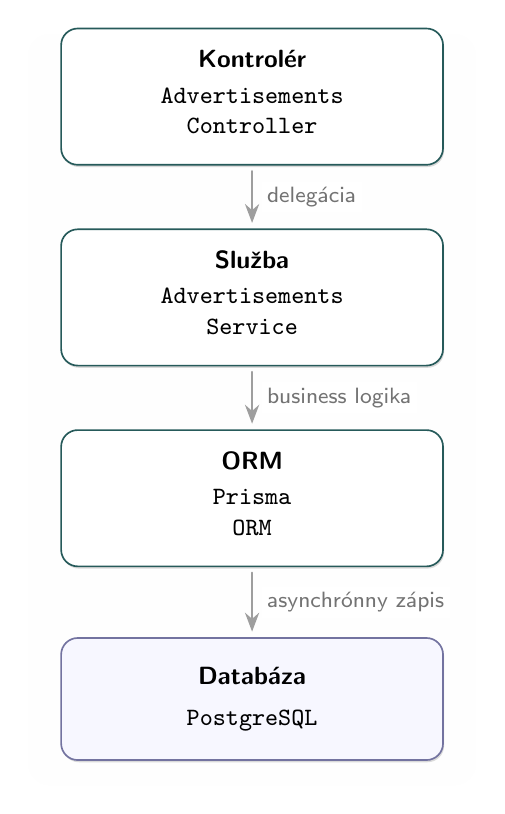
\begin{tikzpicture}[
  font=\sffamily\small,
  line cap=round,
  line join=round,
  >=Stealth,
  layer/.style={
    rectangle,
    rounded corners=6pt,
    minimum width=4.85cm,
    minimum height=1.55cm,
    align=center,
    inner sep=8pt,
    line width=0.6pt,
    draw=teal!48!black!85,
    fill=white,
    drop shadow={
      shadow xshift=0.4pt,
      shadow yshift=-0.8pt,
      opacity=0.14,
      fill=black
    }
  },
  dblayer/.style={
    layer,
    fill=blue!3!white,
    draw=blue!32!black!55
  },
  arr/.style={
    ->,
    line width=0.85pt,
    draw=black!38,
    shorten >=2pt,
    shorten <=2pt
  },
  lbl/.style={
    font=\sffamily\footnotesize,
    text=black!55,
    fill=white,
    inner sep=2pt
  }
]

\begin{scope}[on background layer]
  \fill[blue!1!gray!1, rounded corners=8pt]
    (-0.6, 1.0) rectangle (5.1, -8.55);
\end{scope}

\node[layer] (C) at (2.25, 0.2) {%
  {\bfseries\sffamily Kontrolér}\\[4pt]
  {\small\ttfamily\begin{tabular}{@{}c@{}}Advertisements\\Controller\end{tabular}}%
};
\node[layer] (S) at (2.25, -2.35) {%
  {\bfseries\sffamily Služba}\\[4pt]
  {\small\ttfamily\begin{tabular}{@{}c@{}}Advertisements\\Service\end{tabular}}%
};
\node[layer] (P) at (2.25, -4.9) {%
  {\bfseries\sffamily ORM}\\[4pt]
  {\small\ttfamily\begin{tabular}{@{}c@{}}Prisma\\ORM\end{tabular}}%
};
\node[dblayer] (D) at (2.25, -7.45) {%
  {\bfseries\sffamily Databáza}\\[4pt]
  {\small\ttfamily PostgreSQL}%
};

\draw[arr] (C.south) -- node[lbl, right=3pt, pos=0.5] {delegácia} (S.north);
\draw[arr] (S.south) -- node[lbl, right=3pt, pos=0.5] {business logika} (P.north);
\draw[arr] (P.south) -- node[lbl, right=3pt, pos=0.5] {asynchrónny zápis} (D.north);

\end{tikzpicture}
}
\caption{Tok zápisu dát po validácii: kontrolér, aplikačná služba, Prisma ORM a databáza PostgreSQL}
\label{fig:flow-zapis-databazy}
\end{figure}

\subsection[Databázový model]{Databázový model a entitno-relačný diagram (ERD)}
\noindent
Pre potreby perzistencie dát využívam relačnú databázu \hlcode{PostgreSQL}, ktorá je v rámci vývoja spravovaná pomocou nástroja \hlcode{Prisma ORM} \parencite{obe2017postgresql}. Tento prístup mi umožňuje definovať dátový model v prehľadnom deklaratívnom formáte (\hlcode{schema.prisma}) a následne automaticky generovať migračné skripty a typovo bezpečný klient pre backendovú aplikáciu.

\subsubsection{Hlavné entity systému a ich význam}
\noindent
Logický model databázy pozostáva z niekoľkých kľúčových entít, ktoré sú navzájom prepojené reláciami typu 1:N (one-to-many) alebo M:N (many-to-many).

\begin{itemize}
  \item \textbf{User (Používateľ):} Predstavuje identitu v systéme. Okrem základných údajov ako e-mail a hashované heslo obsahuje informácie o roli (\hlcode{ADMIN} / \hlcode{USER}), firemné údaje pre predajcov (IČO, DIČ, \hlcode{isCompany}), predajný plán (\hlcode{SellerPlan}) a polia súvisiace s moderáciou, ako sú \hlcode{banned}, \hlcode{bannedUntil} a \hlcode{banReason}.

  \item \textbf{Advertisement (Inzerát):} Centrálna entita obsahujúca detaily o ponúkanej službe alebo prenájme (\hlcode{AdvertisementType}). Inzerát je viazaný na konkrétneho autora (používateľa) a kategóriu. Obsahuje stavy definované enumerátorom \hlcode{AdvertisementStatus} (\hlcode{PENDING}, \hlcode{DRAFT}, \hlcode{ACTIVE}, \hlcode{INACTIVE}, \hlcode{ARCHIVED}), lokalitu (GPS súradnice \hlcode{latitude}, \hlcode{longitude}), cenu a špecifikácie uložené vo formáte JSON (\hlcode{specifications}) pre maximálnu flexibilitu parametrov bez nutnosti meniť databázovú schému pri každom novom parametri.

  \item \textbf{Category (Kategória):} Zabezpečuje hierarchické usporiadanie inzerátov. Podporuje vnorenie (parent-child relácie cez \hlcode{parentId}), obsahuje SEO polia (\hlcode{metaTitle}, \hlcode{metaDescription}, \hlcode{slug}) a definuje poradie zobrazenia v navigácii (\hlcode{order}).

  \item \textbf{Filter (Dynamický filter):} Úzko spolupracuje s kategóriami. Definuje, aké dodatočné parametre môže používateľ pri inzeráte v danej kategórii zadať a podľa čoho môže návštevník vyhľadávať. Typy vstupných polí sú definované enumerátorom \hlcode{FilterType}: \hlcode{TEXT}, \hlcode{NUMBER}, \hlcode{SELECT}, \hlcode{MULTISELECT}, \hlcode{BOOLEAN} (áno/nie), \hlcode{DATE} (dátum) a \hlcode{RANGE} (číselný rozsah). Umožňuje tak dynamické rozširovanie vlastností inzerátov podľa ich zaradenia.

  \item \textbf{Message (Správa):} Realizuje komunikačný kanál medzi záujemcom a inzerentom, ale aj systémové notifikácie (\hlcode{MessageType}). Správy sú logicky zoskupované do konverzácií (vlákien) pomocou odkazu na rodičovskú správu (\hlcode{parentId}), čo umožňuje prehľadné zobrazenie chatu v používateľskom rozhraní.

  \item \textbf{Favorite (Obľúbené):} Spojovacia entita realizujúca reláciu M:N medzi používateľom a inzerátmi, ktoré si uložil na neskoršie prehliadnutie.

  \item \textbf{Report (Nahlásenie):} Slúži na moderáciu obsahu. Uchováva informáciu o sťažnosti na konkrétny inzerát, dôvod nahlásenia (\hlcode{ReportReason} -- \hlcode{SPAM}, \hlcode{INAPPROPRIATE}, \hlcode{FAKE}, \hlcode{SCAM}, \hlcode{COPYRIGHT} a \hlcode{OTHER}) a stav riešenia administrátorom (\hlcode{ReportStatus}).

  \item \textbf{Payment (Platba):} Zaznamenáva finančné transakcie medzi záujemcom (\hlcode{renter}) a vlastníkom inzerátu (\hlcode{owner}), pričom sleduje stav platby (\hlcode{PaymentStatus}) a obdobie prenájmu/poskytnutia služby.

  \item \textbf{StaticPage a BlogPost (CMS obsah):} Slúžia na správu obsahu priamo z admin panelu. Obsahujú HTML text, SEO metadáta a stav publikovania (\hlcode{DRAFT} / \hlcode{PUBLISHED}), čím umožňujú administrátorom upravovať informačné podstránky a blog bez zásahu do kódu.

  \item \textbf{ClickEvent (Analytika):} Špeciálna entita určená na zber údajov o správaní používateľov. Zaznamenáva typ interakcie (\hlcode{eventType}), cieľový inzerát alebo kategóriu a segmentačné údaje (pohlavie, typ účtu), čo slúži ako podklad pre administratívne štatistiky a grafy.
\end{itemize}

\subsubsection{Entitno-relačný diagram (ERD)}
\noindent
Logický model databázy som vytvoril v deklaratívnom jazyku Prisma (\hlcode{schema.prisma}), z ktorého následne vyplýva fyzická schéma v PostgreSQL. Obrázok~\ref{fig:erd-database} zobrazuje úplný entitno-relačný diagram so všetkými hlavnými tabuľkami, kľúčmi (PK, FK, UQ) a kardinalitou jednotlivých relácií. Jadrové entity (\hlcode{User}, \hlcode{Advertisement}, \hlcode{Category}) sú vizuálne odlíšené modrastou farbou, podporné a doménové tabuľky sú zobrazené v zelenom (teal) prevedení. Pre zachovanie prehľadnosti diagramu nie sú zobrazené pomocné CMS entity (\hlcode{StaticPage}, \hlcode{BlogPost}, \hlcode{SiteConfig}, \hlcode{SiteMenu}) ani entita \hlcode{AuditLog} pre logovanie administratívnych akcií -- tieto modely nemajú relačné väzby na hlavné domény systému a sú popísané samostatne v texte.

\begin{figure}[p]
\centering
\resizebox{\textwidth}{!}{% Entitno-relačný diagram (ERD) databázy RentMe - portrait, 2 stĺpce
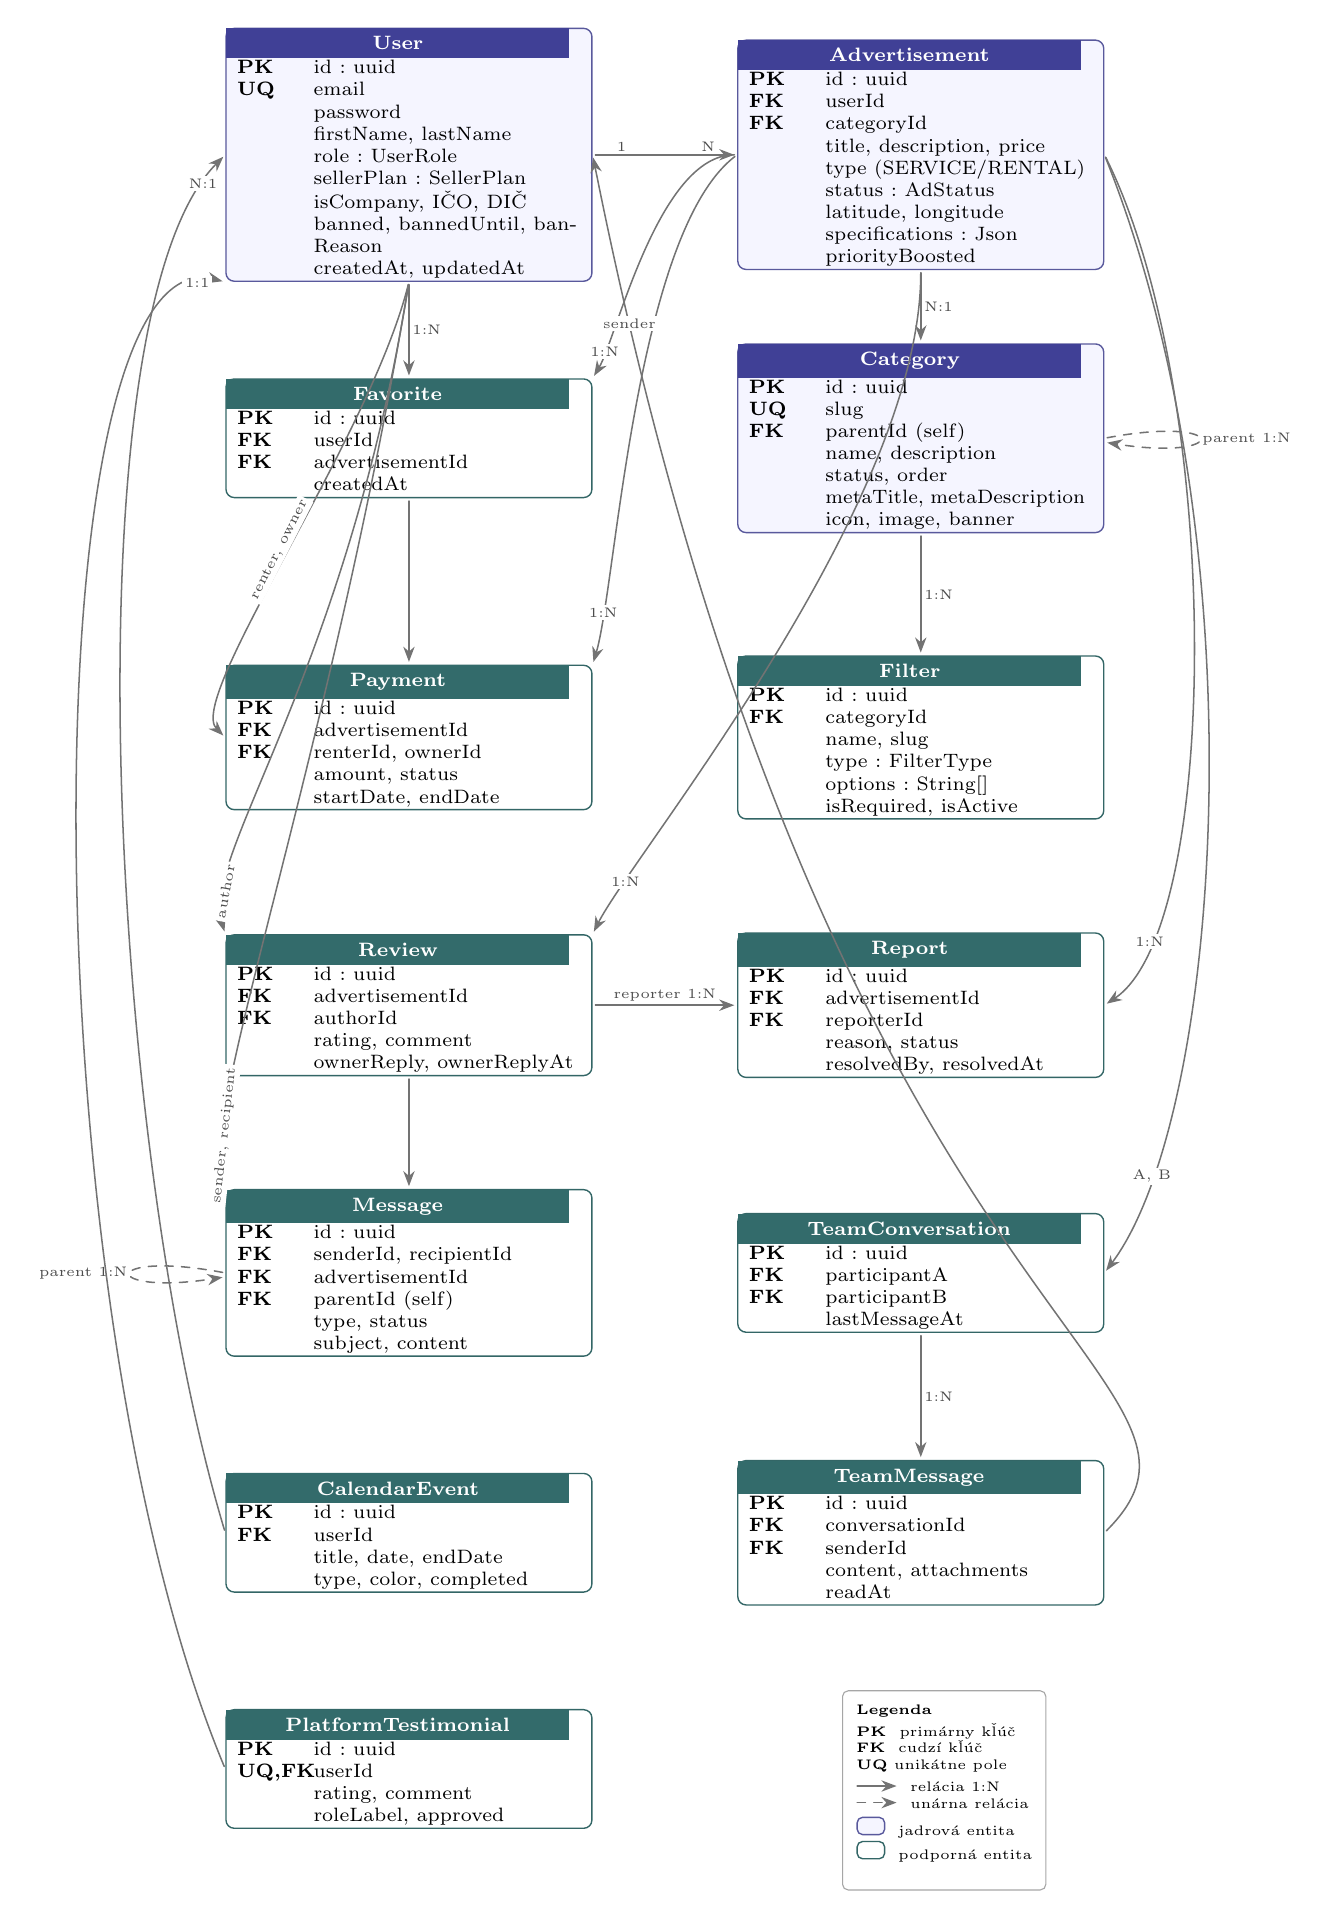
\begin{tikzpicture}[
  font=\rmfamily\scriptsize,
  line cap=round, line join=round,
  >=Stealth,
  entity/.style={
    rectangle, rounded corners=3pt,
    minimum width=4.2cm,
    align=left, inner sep=0pt,
    line width=0.5pt,
    draw=teal!50!black!80, fill=white
  },
  centralent/.style={
    entity,
    draw=blue!40!black!65, fill=blue!4!white
  },
  rel/.style={line width=0.55pt, draw=black!55, shorten >=1pt, shorten <=1pt, ->},
  selfrel/.style={rel, dashed},
  cardlbl/.style={font=\rmfamily\tiny, fill=white, inner sep=1pt, text=black!70}
]

% ========================================================================
% Mriežka 2 stĺpce × 6 riadkov: každá entita má svoju absolútnu pozíciu.
% Ľavý stĺpec x = 0, pravý stĺpec x = 6.5
% Riadky: y = 0, -3.2, -6.0, -8.8, -11.6, -14.4
% ========================================================================

% ─── RIADOK 1: User | Advertisement ─────────────────────────────────────
\node[centralent] (U) at (0, 0) {%
  \begin{tabular}{@{\hspace{4pt}}p{0.55cm}p{3.3cm}@{\hspace{4pt}}}
    \multicolumn{2}{@{}l@{}}{\colorbox{blue!45!black!75}{\parbox{4.15cm}{\centering\color{white}\bfseries User}}}\\[1pt]
    \textbf{PK} & id : uuid \\
    \textbf{UQ} & email \\
        & password \\
        & firstName, lastName \\
        & role : UserRole \\
        & sellerPlan : SellerPlan \\
        & isCompany, IČO, DIČ \\
        & banned, bannedUntil, banReason \\
        & createdAt, updatedAt \\
  \end{tabular}
};

\node[centralent] (A) at (6.5, 0) {%
  \begin{tabular}{@{\hspace{4pt}}p{0.55cm}p{3.3cm}@{\hspace{4pt}}}
    \multicolumn{2}{@{}l@{}}{\colorbox{blue!45!black!75}{\parbox{4.15cm}{\centering\color{white}\bfseries Advertisement}}}\\[1pt]
    \textbf{PK} & id : uuid \\
    \textbf{FK} & userId \\
    \textbf{FK} & categoryId \\
        & title, description, price \\
        & type (SERVICE/RENTAL) \\
        & status : AdStatus \\
        & latitude, longitude \\
        & specifications : Json \\
        & priorityBoosted \\
  \end{tabular}
};

% ─── RIADOK 2: Favorite | Category ──────────────────────────────────────
\node[entity] (Fav) at (0, -3.6) {%
  \begin{tabular}{@{\hspace{4pt}}p{0.55cm}p{3.3cm}@{\hspace{4pt}}}
    \multicolumn{2}{@{}l@{}}{\colorbox{teal!55!black!80}{\parbox{4.15cm}{\centering\color{white}\bfseries Favorite}}}\\[1pt]
    \textbf{PK} & id : uuid \\
    \textbf{FK} & userId \\
    \textbf{FK} & advertisementId \\
        & createdAt \\
  \end{tabular}
};

\node[centralent] (C) at (6.5, -3.6) {%
  \begin{tabular}{@{\hspace{4pt}}p{0.55cm}p{3.3cm}@{\hspace{4pt}}}
    \multicolumn{2}{@{}l@{}}{\colorbox{blue!45!black!75}{\parbox{4.15cm}{\centering\color{white}\bfseries Category}}}\\[1pt]
    \textbf{PK} & id : uuid \\
    \textbf{UQ} & slug \\
    \textbf{FK} & parentId (self) \\
        & name, description \\
        & status, order \\
        & metaTitle, metaDescription \\
        & icon, image, banner \\
  \end{tabular}
};

% ─── RIADOK 3: Payment | Filter ─────────────────────────────────────────
\node[entity] (P) at (0, -7.4) {%
  \begin{tabular}{@{\hspace{4pt}}p{0.55cm}p{3.3cm}@{\hspace{4pt}}}
    \multicolumn{2}{@{}l@{}}{\colorbox{teal!55!black!80}{\parbox{4.15cm}{\centering\color{white}\bfseries Payment}}}\\[1pt]
    \textbf{PK} & id : uuid \\
    \textbf{FK} & advertisementId \\
    \textbf{FK} & renterId, ownerId \\
        & amount, status \\
        & startDate, endDate \\
  \end{tabular}
};

\node[entity] (F) at (6.5, -7.4) {%
  \begin{tabular}{@{\hspace{4pt}}p{0.55cm}p{3.3cm}@{\hspace{4pt}}}
    \multicolumn{2}{@{}l@{}}{\colorbox{teal!55!black!80}{\parbox{4.15cm}{\centering\color{white}\bfseries Filter}}}\\[1pt]
    \textbf{PK} & id : uuid \\
    \textbf{FK} & categoryId \\
        & name, slug \\
        & type : FilterType \\
        & options : String[] \\
        & isRequired, isActive \\
  \end{tabular}
};

% ─── RIADOK 4: Review | Report ──────────────────────────────────────────
\node[entity] (R) at (0, -10.8) {%
  \begin{tabular}{@{\hspace{4pt}}p{0.55cm}p{3.3cm}@{\hspace{4pt}}}
    \multicolumn{2}{@{}l@{}}{\colorbox{teal!55!black!80}{\parbox{4.15cm}{\centering\color{white}\bfseries Review}}}\\[1pt]
    \textbf{PK} & id : uuid \\
    \textbf{FK} & advertisementId \\
    \textbf{FK} & authorId \\
        & rating, comment \\
        & ownerReply, ownerReplyAt \\
  \end{tabular}
};

\node[entity] (Rep) at (6.5, -10.8) {%
  \begin{tabular}{@{\hspace{4pt}}p{0.55cm}p{3.3cm}@{\hspace{4pt}}}
    \multicolumn{2}{@{}l@{}}{\colorbox{teal!55!black!80}{\parbox{4.15cm}{\centering\color{white}\bfseries Report}}}\\[1pt]
    \textbf{PK} & id : uuid \\
    \textbf{FK} & advertisementId \\
    \textbf{FK} & reporterId \\
        & reason, status \\
        & resolvedBy, resolvedAt \\
  \end{tabular}
};

% ─── RIADOK 5: Message | TeamConversation ───────────────────────────────
\node[entity] (M) at (0, -14.2) {%
  \begin{tabular}{@{\hspace{4pt}}p{0.55cm}p{3.3cm}@{\hspace{4pt}}}
    \multicolumn{2}{@{}l@{}}{\colorbox{teal!55!black!80}{\parbox{4.15cm}{\centering\color{white}\bfseries Message}}}\\[1pt]
    \textbf{PK} & id : uuid \\
    \textbf{FK} & senderId, recipientId \\
    \textbf{FK} & advertisementId \\
    \textbf{FK} & parentId (self) \\
        & type, status \\
        & subject, content \\
  \end{tabular}
};

\node[entity] (TC) at (6.5, -14.2) {%
  \begin{tabular}{@{\hspace{4pt}}p{0.55cm}p{3.3cm}@{\hspace{4pt}}}
    \multicolumn{2}{@{}l@{}}{\colorbox{teal!55!black!80}{\parbox{4.15cm}{\centering\color{white}\bfseries TeamConversation}}}\\[1pt]
    \textbf{PK} & id : uuid \\
    \textbf{FK} & participantA \\
    \textbf{FK} & participantB \\
        & lastMessageAt \\
  \end{tabular}
};

% ─── RIADOK 6: CalendarEvent | TeamMessage | PlatformTestimonial ───────
\node[entity] (CE) at (0, -17.5) {%
  \begin{tabular}{@{\hspace{4pt}}p{0.55cm}p{3.3cm}@{\hspace{4pt}}}
    \multicolumn{2}{@{}l@{}}{\colorbox{teal!55!black!80}{\parbox{4.15cm}{\centering\color{white}\bfseries CalendarEvent}}}\\[1pt]
    \textbf{PK} & id : uuid \\
    \textbf{FK} & userId \\
        & title, date, endDate \\
        & type, color, completed \\
  \end{tabular}
};

\node[entity] (TM) at (6.5, -17.5) {%
  \begin{tabular}{@{\hspace{4pt}}p{0.55cm}p{3.3cm}@{\hspace{4pt}}}
    \multicolumn{2}{@{}l@{}}{\colorbox{teal!55!black!80}{\parbox{4.15cm}{\centering\color{white}\bfseries TeamMessage}}}\\[1pt]
    \textbf{PK} & id : uuid \\
    \textbf{FK} & conversationId \\
    \textbf{FK} & senderId \\
        & content, attachments \\
        & readAt \\
  \end{tabular}
};

\node[entity] (PT) at (0, -20.5) {%
  \begin{tabular}{@{\hspace{4pt}}p{0.55cm}p{3.3cm}@{\hspace{4pt}}}
    \multicolumn{2}{@{}l@{}}{\colorbox{teal!55!black!80}{\parbox{4.15cm}{\centering\color{white}\bfseries PlatformTestimonial}}}\\[1pt]
    \textbf{PK} & id : uuid \\
    \textbf{UQ,FK} & userId \\
        & rating, comment \\
        & roleLabel, approved \\
  \end{tabular}
};

% ========================================================================
% Vzťahy
% ========================================================================
% User 1 ──── N Advertisement (vodorovne v R1)
\draw[rel] (U.east) -- node[cardlbl, above, pos=0.2] {1} node[cardlbl, above, pos=0.8] {N} (A.west);

% Advertisement N ──── 1 Category (vodorovne na pravom stĺpci R1->R2)
\draw[rel] (A.south) -- node[cardlbl, right, pos=0.5] {N:1} (C.north);

% Category 1 ──── N Filter (R2->R3)
\draw[rel] (C.south) -- node[cardlbl, right, pos=0.5] {1:N} (F.north);

% Category self-loop (parent/child)
\draw[selfrel] (C.east) .. controls ($(C.east)+(1.6,0.3)$) and ($(C.east)+(1.6,-0.3)$) ..
  node[cardlbl, right, pos=0.5] {parent 1:N} ($(C.east)+(0,-0.05)$);

% User 1 ──── N Favorite (vertikálne ľavý stĺpec)
\draw[rel] (U.south) -- node[cardlbl, right, pos=0.5] {1:N} (Fav.north);

% Advertisement ──── Favorite (diagonála)
\draw[rel] (A.west) .. controls ($(A.west)+(-1.0,0)$) and ($(Fav.north east)+(0.3,0.5)$) ..
  node[cardlbl, pos=0.85] {1:N} (Fav.north east);

% Favorite ──── Payment (vertikálne, ľavý stĺpec)
\draw[rel] (Fav.south) -- node[cardlbl, right, pos=0.5] {} (P.north);

% Advertisement ──── Payment (diagonála)
\draw[rel] (A.west) .. controls ($(A.west)+(-1.3,-1)$) and ($(P.north east)+(0.3,1)$) ..
  node[cardlbl, pos=0.85] {1:N} (P.north east);

% User ──── Payment (renter, owner)
\draw[rel] (U.south) .. controls ($(U.south)+(-0.5,-2)$) and ($(P.west)+(-0.5,0.5)$) ..
  node[cardlbl, pos=0.5, sloped, above] {renter, owner} (P.west);

% Advertisement ──── Review
\draw[rel] (A.south) .. controls ($(A.south)+(0,-3)$) and ($(R.north east)+(0.5,1)$) ..
  node[cardlbl, pos=0.85] {1:N} (R.north east);

% User ──── Review (author)
\draw[rel] (U.south) .. controls ($(U.south)+(-0.8,-5)$) and ($(R.north west)+(-0.3,1)$) ..
  node[cardlbl, pos=0.85, sloped] {author} (R.north west);

% Advertisement ──── Report
\draw[rel] (A.east) .. controls ($(A.east)+(1.5,-3)$) and ($(Rep.east)+(1.5,1)$) ..
  node[cardlbl, pos=0.85] {1:N} (Rep.east);

% User ──── Report (reporter) - z User dole cez ľavý okraj
\draw[rel] (R.east) -- node[cardlbl, above, pos=0.5] {reporter 1:N} (Rep.west);

% User ──── Message (sender/recipient)
\draw[rel] (U.south) .. controls ($(U.south)+(-1,-6)$) and ($(M.north west)+(-0.3,1)$) ..
  node[cardlbl, pos=0.85, sloped] {sender, recipient} (M.north west);

% Advertisement ──── Message
\draw[rel] (R.south) -- node[cardlbl, right, pos=0.5] {} (M.north);

% Message self-loop (parent/replies)
\draw[selfrel] (M.west) .. controls ($(M.west)+(-1.6,0.3)$) and ($(M.west)+(-1.6,-0.3)$) ..
  node[cardlbl, left, pos=0.5] {parent 1:N} ($(M.west)+(0,-0.05)$);

% User ──── TeamConversation (A, B - 2× FK)
\draw[rel] (A.east) .. controls ($(A.east)+(2,-5)$) and ($(TC.east)+(1.5,2)$) ..
  node[cardlbl, pos=0.85] {A, B} (TC.east);

% TeamConversation ──── TeamMessage (vertikálne)
\draw[rel] (TC.south) -- node[cardlbl, right, pos=0.5] {1:N} (TM.north);

% TeamMessage ──── User (sender) - dlhý oblúk
\draw[rel] (TM.east) .. controls ($(TM.east)+(2,2)$) and ($(U.east)+(3,-15)$) ..
  node[cardlbl, pos=0.95] {sender} (U.east);

% CalendarEvent ──── User
\draw[rel] (CE.west) .. controls ($(CE.west)+(-1.5,5)$) and ($(U.west)+(-2,-2)$) ..
  node[cardlbl, pos=0.95] {N:1} (U.west);

% PlatformTestimonial ──── User (1:1)
\draw[rel] (PT.west) .. controls ($(PT.west)+(-2.5,6)$) and ($(U.west)+(-2.5,-1)$) ..
  node[cardlbl, pos=0.95] {1:1} (U.south west);

% ========================================================================
% Legenda
% ========================================================================
\node[draw=black!35, fill=white, rounded corners=2pt, inner sep=5pt,
      font=\rmfamily\tiny, align=left,
      anchor=north west]
  at (5.5, -19.5)
{%
  \textbf{Legenda}\\[2pt]
  \textbf{PK}\ \ primárny kľúč\\
  \textbf{FK}\ \ cudzí kľúč\\
  \textbf{UQ}\ unikátne pole\\[2pt]
  \tikz\draw[line width=0.55pt, draw=black!55, >=Stealth, ->] (0,0) -- (0.5,0); \ relácia 1:N\\
  \tikz\draw[dashed, line width=0.55pt, draw=black!55, >=Stealth, ->] (0,0) -- (0.5,0); \ unárna relácia\\[2pt]
  \tikz\draw[fill=blue!4!white, draw=blue!40!black!65, line width=0.5pt] (0,0) rectangle (0.35,0.22); \ jadrová entita\\
  \tikz\draw[fill=white, draw=teal!50!black!80, line width=0.5pt] (0,0) rectangle (0.35,0.22); \ podporná entita\\
};

\end{tikzpicture}
}
\caption{Entitno-relačný diagram (ERD) databázy -- jadrové entity, podporné tabuľky a ich relácie}
\label{fig:erd-database}
\end{figure}

\noindent
Vybrané charakteristické relácie:

\begin{itemize}
  \item Relácia medzi \hlcode{User} a \hlcode{Advertisement} je typu \textbf{1:N} -- jeden používateľ môže vytvoriť viacero inzerátov, no inzerát patrí vždy jednému autorovi.
  \item \hlcode{Category} a \hlcode{Advertisement} tvoria vzťah \textbf{1:N}, kde každá kategória zastrešuje množinu inzerátov.
  \item \hlcode{Category} obsahuje aj \textbf{unárnu reláciu 1:N} sama na seba (cez \hlcode{parentId}), čím vzniká stromová štruktúra hlavných a podriadených kategórií.
  \item \hlcode{Filter} je viazaný na konkrétnu kategóriu (1:N) a definuje dynamické vlastnosti inzerátov v tejto kategórii.
  \item \hlcode{Favorite} predstavuje klasickú dekompozíciu vzťahu \textbf{M:N} medzi používateľom a inzerátom.
  \item \hlcode{Payment} prepája inzerát s dvoma používateľmi (\hlcode{renter} a \hlcode{owner}), čo vytvára komplexnejšiu sieť vzťahov nad tabuľkou používateľov.
  \item \hlcode{Message} obsahuje vlastnú \textbf{unárnu reláciu} (\hlcode{parentId} $\to$ \hlcode{replies}), ktorá umožňuje hierarchické zoraďovanie odpovedí do vlákien konverzácií.
  \item \hlcode{TeamConversation} viaže vždy dvoch používateľov cez polia \hlcode{participantA} a \hlcode{participantB} (dve nezávislé 1:N relácie), pričom unikátnym obmedzením je zaručené, že medzi dvoma účastníkmi existuje vždy najviac jedna konverzácia.
  \item \hlcode{PlatformTestimonial} má voči \hlcode{User} reláciu \textbf{1:1} -- jeden používateľ môže mať najviac jednu verejnú referenciu zobrazenú na homepage.
\end{itemize}

\noindent
Anotácie \hlcode{@@index} v Prisma schéme explicitne deklarujú indexy nad poliami, ktoré sa najčastejšie objavujú v podmienkach \hlcode{WHERE} (\hlcode{status}, \hlcode{slug}, \hlcode{categoryId}, \hlcode{userId}, \hlcode{createdAt}), čím sa zaručuje predvídateľný výkon dopytov aj pri raste objemu dát. Klauzuly \hlcode{onDelete: Cascade} a \hlcode{onDelete: SetNull} explicitne riadia referenčnú integritu na úrovni databázy -- odstránenie agregátneho koreňa (napr. používateľa) automaticky odstráni alebo zneplatní viazané záznamy bez nutnosti špeciálnej aplikačnej logiky.

\subsection[REST API a JWT]{Návrh REST API rozhrania a autentifikačného mechanizmu (JWT)}
\noindent
Komunikácia v systéme prebieha prostredníctvom REST API (Representational State Transfer), ktoré využíva protokol HTTP a formát JSON na výmenu údajov. API je navrhnuté ako bezstavové, čo znamená, že každá požiadavka od klienta musí obsahovať všetky informácie potrebné na jej spracovanie, vrátane overenia identity \parencite{richardson2013restful}.

\subsubsection{Návrh endpointov a smerovania}
\noindent
API je logicky rozdelené do modulov, ktoré zodpovedajú doménam v databáze. Každý modul definuje sadu koncových bodov (endpointov) pre operácie CRUD (Create, Read, Update, Delete) a špecifickú biznis logiku.

\begin{table}[htbp]
\centering
\begingroup
\footnotesize
\setlength{\tabcolsep}{6.5pt}
\renewcommand{\arraystretch}{1.38}
\rowcolors{2}{gray!7}{white}
\begin{tabular}{@{}>{\raggedright\arraybackslash}p{0.165\linewidth}>{\raggedright\arraybackslash}p{0.235\linewidth}>{\raggedright\arraybackslash}p{0.515\linewidth}@{}}
\toprule
\rowcolor{gray!14}
\textbf{Modul} & \textbf{Základná cesta} & \textbf{Významné operácie} \\
\midrule
\textbf{Auth} & \hlcode{/auth} & Registrácia, prihlásenie, získanie profilu prihláseného používateľa. \\
\textbf{Users} & \hlcode{/users} & Správa používateľských profilov, zmena hesla a osobných údajov. \\
\textbf{Advertise\-ments} & \hlcode{/advertisements} & Vyhľadávanie, tvorba inzerátov, schvaľovanie (admin), mapa. \\
\textbf{Categories} & \hlcode{/categories} & Hierarchická správa kategórií, prepojenie na dynamické filtre. \\
\textbf{Filters} & \hlcode{/filters} & Dynamické filtre per kategória (typy \hlcode{TEXT}, \hlcode{NUMBER}, \hlcode{SELECT}, \hlcode{MULTISELECT}, \hlcode{BOOLEAN}, \hlcode{DATE}, \hlcode{RANGE}). \\
\textbf{Messages} & \hlcode{/messages} & Odosielanie dopytov, správa konverzácií a chat. \\
\textbf{Favorites} & \hlcode{/favorites} & Pridávanie a odoberanie inzerátov z obľúbených (relácia M:N). \\
\textbf{Reports} & \hlcode{/reports} & Nahlasovanie inzerátov, moderátorské workflow. \\
\textbf{Reviews} & \hlcode{/reviews} & Hodnotenia inzerátov, odpovede vlastníkov. \\
\textbf{Admin} & \hlcode{/admin} & Agregované štatistiky, moderácia obsahu a banovanie účtov. \\
\textbf{Analytics} & \hlcode{/analytics} & Zaznamenávanie kliknutí (\hlcode{/analytics/click}) a generovanie reportov. \\
\textbf{CMS} & \hlcode{/static-pages}, \hlcode{/blog} & Statické stránky a blogové príspevky spravované cez admin panel. \\
\bottomrule
\end{tabular}
\endgroup
\caption{Prehľad hlavných modulov API a základných ciest}
\label{tab:api-moduly}
\end{table}

Všetky endpointy sú zdokumentované pomocou nástroja Swagger, ktorý je prístupný na adrese \hlcode{GET /api/docs}. Táto dokumentácia slúži ako kontrakt medzi backendom a frontendovými tímami (v tomto prípade aplikáciami \hlcode{platform}, \hlcode{user} a \hlcode{admin}).

\subsubsection{Autentifikačný mechanizmus (JWT)}
\noindent
Na zabezpečenie prístupu k chráneným zdrojom využíva platforma JSON Web Token (JWT) \parencite{jones2015jwt}. Tento mechanizmus umožňuje overiť identitu používateľa bez nutnosti ukladať informácie o relácii (session) na serveri.

\textbf{Proces autentifikácie a autorizácie:}

\begin{enumerate}
  \item \textbf{Prihlásenie:} Používateľ odošle prihlasovacie údaje na \hlcode{/auth/login}. Server overí heslo (pomocou \hlcode{bcrypt} s 10 salt rounds) a ak je správne, vygeneruje podpísaný JWT token.
  \item \textbf{Payload tokenu:} Token obsahuje zakódované informácie ako \hlcode{userId}, \hlcode{email} a \hlcode{role} (\hlcode{ADMIN} alebo \hlcode{USER}).
  \item \textbf{Autorizované požiadavky:} Klient ukladá token a posiela ho v hlavičke každého ďalšieho volania: \texttt{Authorization: Bearer \textless token\textgreater}.
  \item \textbf{Validácia na serveri:} API využíva \hlcamel{JwtAuth}{Guard} na overenie podpisu tokenu a \hlcamel{Roles}{Guard} na kontrolu, či má používateľ dostatočné oprávnenia (napr. prístup do admin panelu).
\end{enumerate}

\subsubsection{Validácia a transformácia údajov}
\noindent
Pre zabezpečenie integrity systému je každá prichádzajúca požiadavka validovaná pomocou DTO (Data Transfer Objects). Využitie globálneho \hlcode{ValidationPipe} v \hlcode{NestJS} zabezpečuje:

\begin{itemize}
  \item \textbf{Whitelist:} Odstránenie polí, ktoré nie sú definované v DTO, čím sa bráni neoprávneným zmenám v databáze.
  \item \textbf{Transformácia:} Automatický prevod reťazcov z URL parametrov na číselné typy alebo objekty, čo zjednodušuje prácu v službách (services).
\end{itemize}

\subsubsection{Spracovanie chýb (Error Handling)}
\noindent
API využíva štandardizované HTTP status kódy (napr. \hlcode{400 Bad Request} pre chyby validácie, \hlcode{401 Unauthorized} pre neautorizovaný prístup, \hlcode{403 Forbidden} pre nedostatočné práva a \hlcode{404 Not Found} pre nenájdené zdroje). Systém vracia jednotný formát chybových hlásení vo formáte JSON, čo umožňuje ich ľahšie a konzistentné spracovanie na strane klientskych aplikácií (frontendu).

\noindent
Tento návrh API a bezpečnosti zaručuje, že platforma je robustná, odolná voči bežným útokom a pripravená na komunikáciu s rôznymi typmi klientskych zariadení.

\section{Metodika a použité technológie}
\noindent
Pri vývoji komplexnej inzertnej platformy som zvolil prístup, ktorý kladie dôraz na rýchlosť vývoja, bezpečnosť kódu a jednoduchú údržbu. Celý ekosystém je postavený na moderných JavaScriptových technológiách, ktoré umožňujú zdieľanie logiky medzi serverovou a klientskou časťou.

\subsection{Full-stack vývoj v jazyku TypeScript}
\noindent
Základným stavebným kameňom celého projektu je jazyk \emph{TypeScript} \parencite{cherny2019typescript}. Ide o nadstavbu JavaScriptu, ktorá do dynamického sveta webového vývoja prináša statické typovanie. Pre projekt tohto rozsahu, kde komunikujú tri frontendové aplikácie s jedným API, je použitie TypeScriptu kľúčovým rozhodnutím z niekoľkých dôvodov:

\subsubsection{Typová bezpečnosť a eliminácia chýb}
\noindent
TypeScript umožňuje definovať presné štruktúry dát (rozhrania a typy) už počas písania kódu. Vďaka tomu dokáže vývojové prostredie (IDE) okamžite upozorniť na chyby, ktoré by sa v čistom JavaScripte prejavili až počas behu aplikácie (napr. prístup k neexistujúcemu poľu objektu). V projekte sú takto ošetrené všetky kľúčové entity, ako sú inzeráty, používatelia či správy. Zatiaľ čo TypeScript zabezpečuje internú konzistenciu kódu počas vývoja (\emph{compile-time}), v kombinácii s knižnicou \hlcode{class-validator} na backende garantuje, že do systému nevstúpia nevalidné dáta ani z externých HTTP požiadaviek (\emph{runtime}).

\subsubsection{Zdieľanie kódu v monorepe}
\noindent
Využitie TypeScriptu v prostredí monorepa mi dovoľuje vytvoriť balík \hlcode{packages/shared}, kde sú definované DTO (\emph{Data Transfer Objects}). Tieto objekty slúžia ako záväzný kontrakt medzi backendom a frontendom.

Keď v \hlcode{api} zmením štruktúru odpovede pre detail inzerátu, TypeScript ma v aplikáciách \hlcode{platform} alebo \hlcode{admin} automaticky upozorní na všetkých miestach, kde je potrebné kód aktualizovať.

Tento mechanizmus zabezpečuje \emph{end-to-end} typovú bezpečnosť, čo dramaticky zvyšuje stabilitu systému pri zmenách v databázovom modeli.

\noindent\textit{Príklad zdieľaného DTO v balíku \hlcode{packages/shared} (využitie tried pre runtime validáciu):}

\noindent\begin{minipage}{\linewidth}
\begin{lstlisting}[
  language=Java,
  basicstyle=\ttfamily\footnotesize\color{vscText},
  breaklines=true,
  breakatwhitespace=true
]
import {
  IsString, IsOptional, IsNumber,
} from 'class-validator';

export class CreateAdvertisementDto {
  @IsString()
  title: string;

  @IsString()
  description: string;

  @IsOptional()
  @IsNumber()
  price?: number;

  // ...
}
\end{lstlisting}
\end{minipage}
\vspace{0.4\baselineskip}
\noindent\small\textit{Poznámka: V NestJS sa pre DTO odporúča používať triedy (\texttt{class}) namiesto rozhraní (\texttt{interface}). Dôvodom je, že rozhrania v JavaScripte po kompilácii úplne zmiznú, kým triedy zostávajú zachované aj v \emph{runtime}.}\par
\noindent\small\textit{To umožňuje knižniciam ako \hlcode{class-validator} alebo Swagger čítať metadáta o typoch polí.}\normalsize

\subsubsection{Lepšia čitateľnosť, dokumentácia a Developer Experience (DX)}
\noindent
Kód napísaný v TypeScripte je v podstate „samodokumentovateľný“. Akýkoľvek iný vývojár (alebo administrátor systému) dokáže z definícií typov okamžite pochopiť, aké dáta funkcia prijíma a čo vracajú jednotlivé API endpointy. To je dôležité najmä pri modulárnej architektúre NestJS, kde sú jednotlivé služby a kontroléry jasne definované pomocou dekorátorov a typov.

Zároveň TypeScript výrazne zlepšuje \emph{Developer Experience (DX)} vďaka autokompletizácii (IntelliSense) v moderných IDE (ako je VS Code). Pre vývojára to znamená, že nemusí neustále prepínať okná a pozerať sa do databázovej schémy, pretože mu editor sám našepkáva dostupné polia inzerátu alebo používateľa.

\subsubsection{Moderné funkcie, dekorátory a kompatibilita}
\noindent
TypeScript mi umožňuje využívať najnovšie funkcie jazyka ECMAScript (ako asynchrónne funkcie, deštrukturalizáciu či voliteľné reťazenie), ktoré sú následne kompilované do optimalizovaného JavaScriptu. To zaručuje, že aplikácia beží efektívne v prostredí Node.js na serveri aj v moderných webových prehliadačoch.

Keďže backend využíva NestJS, naplno sa tu prejavuje sila TypeScriptu aj cez dekorátory (\hlcode{@Controller}, \hlcode{@Get}, \hlcode{@Injectable}). Tie umožňujú reflexiu metadát, čo je pokročilá funkcia, vďaka ktorej NestJS vie, ako poskladať závislosti (\emph{Dependency Injection}).

\subsection{Backend: Framework NestJS a modulárna architektúra}
\noindent
Backendová časť aplikácie (\hlcode{apps/api}) je vyvinutá v prostredí NestJS. Ide o progresívny framework pre Node.js \parencite{casciaro2020nodejs}, ktorý využíva TypeScript a kombinuje prvky objektovo orientovaného programovania, funkcionálneho programovania a reaktívneho programovania.

\subsubsection{Modulárna štruktúra a organizácia kódu}
\noindent
Hlavnou výhodou NestJS je jeho striktná modulárna architektúra \parencite{martin2017cleanarch}. Každá logická časť platformy je zapuzdrená do samostatného modulu, ktorý obsahuje vlastné kontroléry, služby a dátové modely.

\begin{itemize}
  \item \textbf{Zapuzdrenie logiky:} Napríklad \hlcode{AdvertisementsModule} sa stará výhradne o inzeráty, zatiaľ čo \hlcode{AuthModule} rieši autentifikáciu. Tieto moduly sú navzájom nezávislé a striktne dodržiavajú princíp jednej zodpovednosti (\emph{Single Responsibility Principle} -- SRP), čo uľahčuje testovanie a umožňuje pridávanie nových funkcií (napr. platobný modul) bez rizika narušenia existujúceho kódu. Všetky tieto doménové moduly sú následne spojené do jedného hlavného stromu aplikácie prostredníctvom koreňového modulu (\hlcode{app.module.ts}).
  \item \textbf{Dekorátory a metadáta:} NestJS intenzívne využíva dekorátory (napr. \hlcode{@Get()}, \hlcode{@Post()}, \hlcode{@UseGuards()}), ktoré robia kód čitateľnejším a deklaratívnym. Už na prvý pohľad je jasné, ktorý endpoint je verejný a ktorý vyžaduje administrátorské oprávnenia.
\end{itemize}

\noindent\textit{Príklad použitia dekorátorov v kontroléri (ukážka z \hlcode{AdvertisementsController}):}

\noindent\begin{minipage}{\linewidth}
\begin{lstlisting}[
  language=Java,
  basicstyle=\ttfamily\footnotesize\color{vscText},
  breaklines=true,
  breakatwhitespace=true
]
@Controller('advertisements')
export class AdvertisementsController {
  constructor(private readonly advertisementsService: AdvertisementsService) {}

  @Get('pending/all')
  @UseGuards(JwtAuthGuard, RolesGuard)
  @Roles(UserRole.ADMIN)
  findPending() {
    return this.advertisementsService.findPending();
  }
}
\end{lstlisting}
\end{minipage}
\vspace{0.4\baselineskip}
\noindent
V tejto ukážke je jasne vidieť, ako dekorátory \hlcode{@UseGuards} a \hlcode{@Roles} zabezpečujú ochranu endpointu tak, aby k nemu mal prístup iba administrátor.

\subsubsection{Dependency Injection (Injektovanie závislostí)}
\noindent
Framework využíva návrhový vzor \emph{Dependency Injection} (DI), ktorý automatizuje správu inštancií tried \parencite{martin2017cleanarch}.

V praxi to znamená, že ak služba \hlcode{AdvertisementsService} potrebuje pristupovať k databáze cez \hlcode{PrismaService}, stačí túto závislosť definovať v konštruktore a NestJS sa postará o jej vytvorenie a prepojenie.

Tento prístup zvyšuje modularitu a umožňuje jednoduchú výmenu komponentov, čo je v súlade s princípmi čistého kódu (\emph{Clean Code}).

\subsubsection{Middleware a Guardy pre bezpečnosť}
\noindent
NestJS poskytuje robustný systém na spracovanie životného cyklu požiadavky (\emph{Request Lifecycle}) \parencite{casciaro2020nodejs}. Každá prichádzajúca HTTP požiadavka prechádza presne definovanou cestou: najprv sa vykoná \emph{Middleware}, následne \emph{Guards} (strážcovia prístupu), \emph{Interceptors} (zachytávače), \emph{Pipes} (validácia a transformácia dát), až sa nakoniec dostane do samotného kontroléra a služby. Tento jasne štruktúrovaný tok umožňuje oddeliť biznis logiku od infraštruktúrnych a bezpečnostných úloh.

\begin{itemize}
  \item \textbf{Guards (Strážcovia):} Využívam ich na ochranu endpointov. \hlcode{JwtAuthGuard} overuje platnosť tokenu a \hlcode{RolesGuard} kontroluje, či má používateľ rolu \hlcode{ADMIN}.
  \item \textbf{Interceptors a Pipes:} Tieto nástroje slúžia na transformáciu dát (napr. úprava formátu odpovede) a ich validáciu. Vďaka \hlcode{ValidationPipe} je zaručené, že do systému sa nedostanú nekorektné dáta, ktoré by mohli spôsobiť pád aplikácie alebo bezpečnostnú dieru.
\end{itemize}

\subsubsection{Integrácia s Prisma ORM}
\noindent
NestJS sa výborne dopĺňa s nástrojom Prisma. V projekte som vytvoril dedikovaný \hlcode{PrismaModule}, ktorý spracováva pripojenie k PostgreSQL databáze. Služba \hlcode{PrismaService} priamo rozširuje triedu \hlcode{PrismaClient} a využíva zabudované hooky životného cyklu NestJS, konkrétne \hlcode{onModuleInit}. Vďaka tomu sa spojenie s databázou nadviaže hneď pri štarte aplikácie, čo zaručuje, že API nezačne prijímať požiadavky skôr, než je databáza plne pripravená.

Prisma funguje ako typovo bezpečný most (ORM), ktorý mi umožňuje pracovať s databázou pomocou bežných TypeScript objektov namiesto písania surových SQL dopytov.

Výsledkom je kód, ktorý je menej náchylný na chyby a oveľa rýchlejšie sa vyvíja.

\subsection{Frontend: Next.js (App Router), React a Tailwind CSS}
\noindent
Frontendová architektúra pozostáva z troch samostatných aplikácií (\hlcode{platform}, \hlcode{user}, \hlcode{admin}), ktoré zdieľajú rovnaký technologický základ. Tento prístup umožňuje izolovať používateľské rozhrania podľa ich účelu, pričom sa zachováva konzistentný vývojový proces.

\subsubsection{Next.js a architektúra App Router}
\noindent
Použitie Next.js (verzia 16+) prináša do projektu revolučný prístup k vykresľovaniu stránok prostredníctvom App Routera.

\begin{itemize}
  \item \textbf{React Server Components (RSC):} Väčšina komponentov je predvolene vykresľovaná na strane servera. To znamená, že klient dostane hotový HTML dokument, čo dramaticky zrýchľuje prvé načítanie stránky a zlepšuje SEO, keďže vyhľadávače nemusia spúšťať zložitý JavaScript, aby videli obsah inzerátov. Okrem výkonu prinášajú RSC aj bezpečnostné výhody -- umožňujú pristupovať k citlivým dátam alebo premenným prostredia (napr. API kľúčom) priamo na serveri bez toho, aby boli tieto údaje odoslané do prehliadača klienta.
  \item \textbf{Smerovanie (File-based Routing):} Next.js využíva adresárovú štruktúru na definovanie trás. Vďaka tomu je navigácia v aplikácii intuitívna a podporuje pokročilé funkcie ako paralelné trasy alebo interceptovanie trás (napr. zobrazenie detailu inzerátu v modálnom okne bez straty kontextu zoznamu).
  \item \textbf{Optimalizácia:} Framework automaticky optimalizuje obrázky, fonty a skripty, čo zabezpečuje plynulý chod aplikácie aj na slabších mobilných zariadeniach.
\end{itemize}

\subsubsection{Deklaratívne UI s knižnicou React}
\noindent
Samotné používateľské rozhranie je postavené na knižnici React \parencite{riva2022nextjs}. Využívam moderné koncepty ako Hooks (\hlcode{useState}, \hlcode{useEffect}, \hlcode{useMemo}) na správu stavu a vedľajších účinkov.

\begin{itemize}
  \item \textbf{Komponentový prístup:} Každý prvok rozhrania (tlačidlo, karta inzerátu, vyhľadávací panel) je samostatný znovupoužiteľný komponent. To uľahčuje údržbu kódu a zabezpečuje vizuálnu jednotnosť naprieč všetkými tromi aplikáciami v monorepe.
\end{itemize}

\noindent\textit{Príklad komponentu s využitím podmienkového renderovania a Tailwind CSS (ukážka z \hlcode{CreateAdvertisementWizard}):}

\noindent\begin{minipage}{\linewidth}
\begin{lstlisting}[
  language=TSX,
  basicstyle=\ttfamily\footnotesize\color{vscText},
  columns=fullflexible,
  keepspaces=true,
  breaklines=true,
  breakatwhitespace=false
]
function CategoryVisualTile({ cat, selected, onSelect, tileVariant = 'platform' }) {
  const isAdmin = tileVariant === 'admin';
  return (
    <button
      type="button"
      onClick={onSelect}
      className={
        isAdmin
          ? `group flex flex-col items-center rounded-xl border-2 bg-card px-2 py-5 text-center transition-all ${
              selected ? 'border-primary ring-2 ring-primary/25' : 'border-card hover:border-primary/40'
            }`
          : `group flex flex-col items-center rounded-2xl border-2 bg-white px-2 py-5 text-center transition-all ${
              selected ? 'border-[#1dbf73] ring-2 ring-[#1dbf73]/25' : 'border-white/80 hover:border-[#1dbf73]/40'
            }`
      }
    >
      <span className={isAdmin ? 'text-white' : 'text-gray-900'}>{cat.name}</span>
    </button>
  );
}
\end{lstlisting}
\end{minipage}
\vspace{0.4\baselineskip}
\noindent
Táto ukážka demonštruje, ako jeden komponent dokáže dynamicky meniť svoj vzhľad na základe toho, či je vykresľovaný vo verejnej platforme alebo v administrátorskom rozhraní.

\begin{itemize}
  \item \textbf{Klientska interaktivita a hydratácia:} Kým jadro stránky je serverové, interaktívne prvky (napr. chat, mapové filtre alebo formuláre) využívajú klientske komponenty (označené direktívou \texttt{'use client'}). Pri kombinácii týchto prístupov dochádza k procesu zvanému \emph{hydratácia}. Next.js najprv pošle na klienta statické HTML pre rýchle zobrazenie obsahu a následne toto rozhranie „oživí“ pomocou JavaScriptu, čím sa dosiahne plná interaktivita a okamžitá odozva na akcie používateľa.
\end{itemize}

\subsubsection{Styling pomocou Tailwind CSS}
\noindent
Na definovanie vizuálnej identity platformy som zvolil Tailwind CSS, čo je \emph{utility-first} CSS framework \parencite{riva2022nextjs}.

\begin{itemize}
  \item \textbf{Rýchlosť vývoja a purging:} Namiesto písania tisícok riadkov v samostatných CSS súboroch definujem štýly priamo v HTML/JSX pomocou predpripravených tried. Tailwind počas zostavovania (\emph{build}) aplikácie analyzuje zdrojové súbory a do výsledného CSS zahrnie iba tie triedy, ktoré sú skutočne použité. Tento proces (scanning/purging) eliminuje „mŕtvy kód“ (\emph{dead code}) a výsledný štýl pre celú platformu má často veľkosť len niekoľko desiatok kilobajtov.
  \item \textbf{Responzivita a Mobile-first:} Tailwind natívne podporuje responzívny dizajn. Vďaka tomu bolo možné jednoducho implementovať rozhranie, ktoré sa automaticky prispôsobuje od malých displejov smartfónov až po veľké desktopové monitory.
  \item \textbf{Konzistencia:} Využitie konfiguračného súboru \hlcode{tailwind.config.js} zabezpečuje, že farby, písma a rozostupy sú identické vo všetkých aplikáciách, čo buduje profesionálny dojem z platformy.
\end{itemize}

\subsubsection{Integrácia s mapovými podkladmi (Leaflet)}
\noindent
Pre inzertný portál je kľúčová vizualizácia polohy. Vo fronte aplikácie \hlcode{platform} využívam knižnicu Leaflet v kombinácii s React komponentmi. Táto integrácia umožňuje návštevníkom dynamicky prehliadať inzeráty na interaktívnej mape, pričom dáta o polohe (latitúda a longitúda) sú v reálnom čase sťahované z NestJS API. Globálny pohľad na mapu so všetkými aktívnymi inzerátmi reprezentovanými ako interaktívne markery dokumentuje obrázok~\ref{fig:mapa-1}.

\begin{figure}[htbp]
\centering
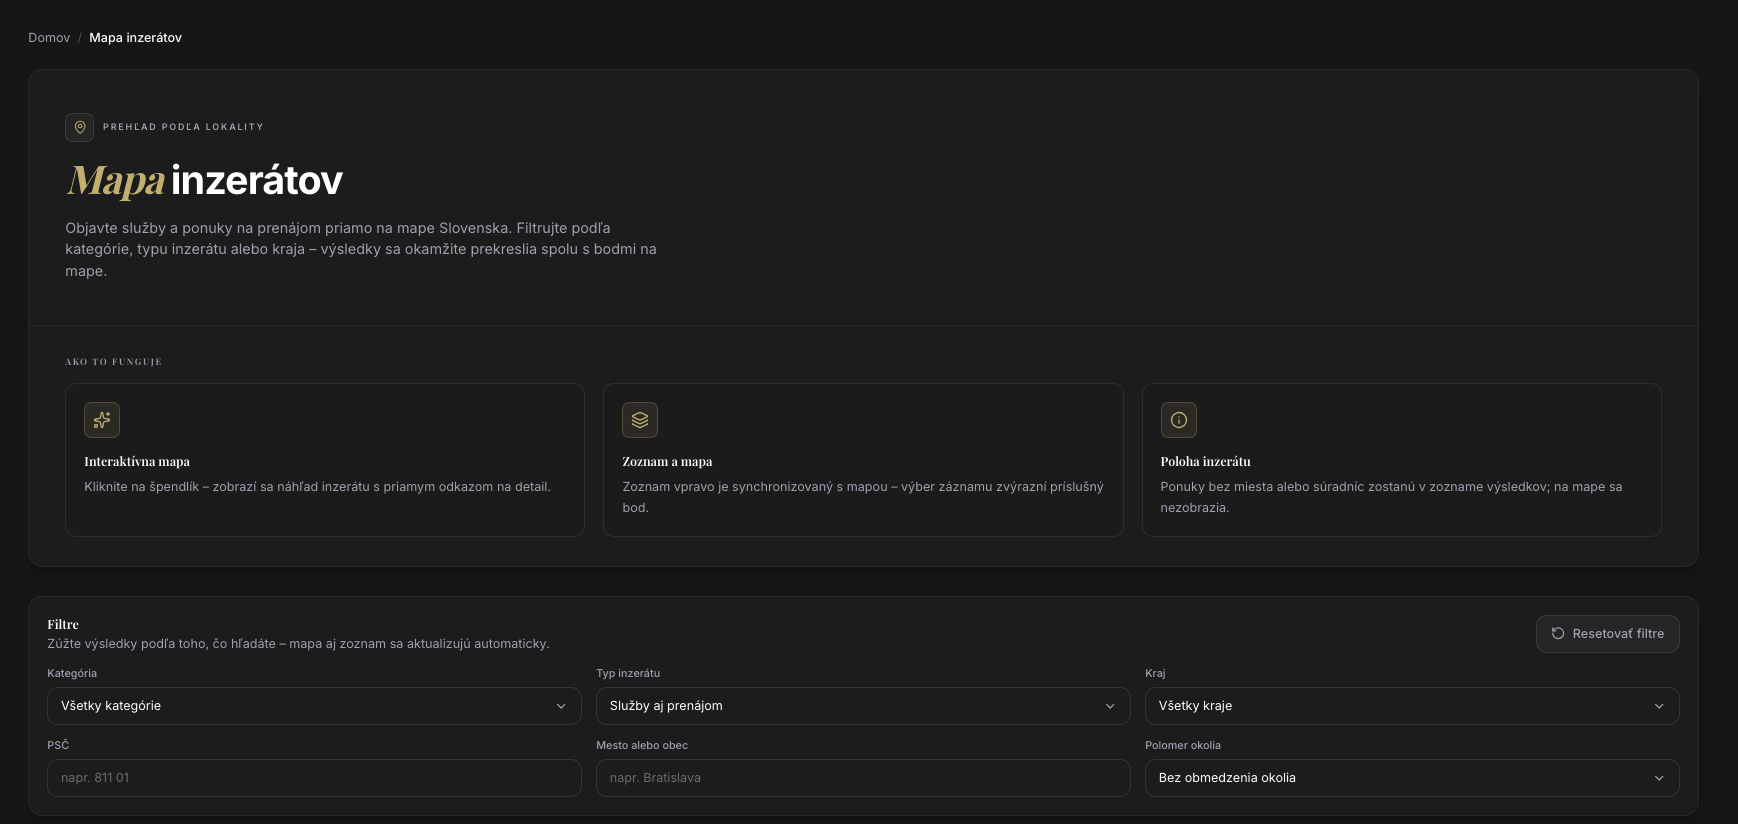
\includegraphics[width=\textwidth]{images/mapa_1.png}
\caption{Mapové zobrazenie inzerátov (Leaflet) -- markery agregované do clusterov pri väčšom priblížení a dynamické načítanie polôh z endpointu \texttt{GET /advertisements/map}}
\label{fig:mapa-1}
\end{figure}

Keďže knižnice ako Leaflet pracujú priamo s objektom \hlcode{window}, ktorý na serveri neexistuje, bolo nutné vyriešiť kompatibilitu so Server-Side Renderingom (SSR). V Next.js sa takéto klientske knižnice načítavajú asynchrónne pomocou funkcie \texttt{dynamic} z modulu \texttt{next/dynamic}, typicky zápisom v tvare:\par
\nobreak\noindent{\small\texttt{dynamic(() => import(...), \{ ssr: false \})}}\par
\nobreak\noindent
Toto riešenie zabezpečí, že sa mapa inicializuje až priamo v prehliadači používateľa, čím sa predíde chybám pri renderovaní na serveri. Pri kliknutí na konkrétny marker sa zobrazí detailný popup s náhľadom inzerátu, ako je znázornené na obrázku~\ref{fig:mapa-2}; popup obsahuje fotografiu, názov, cenu a odkaz na plný detail ponuky.

\begin{figure}[htbp]
\centering
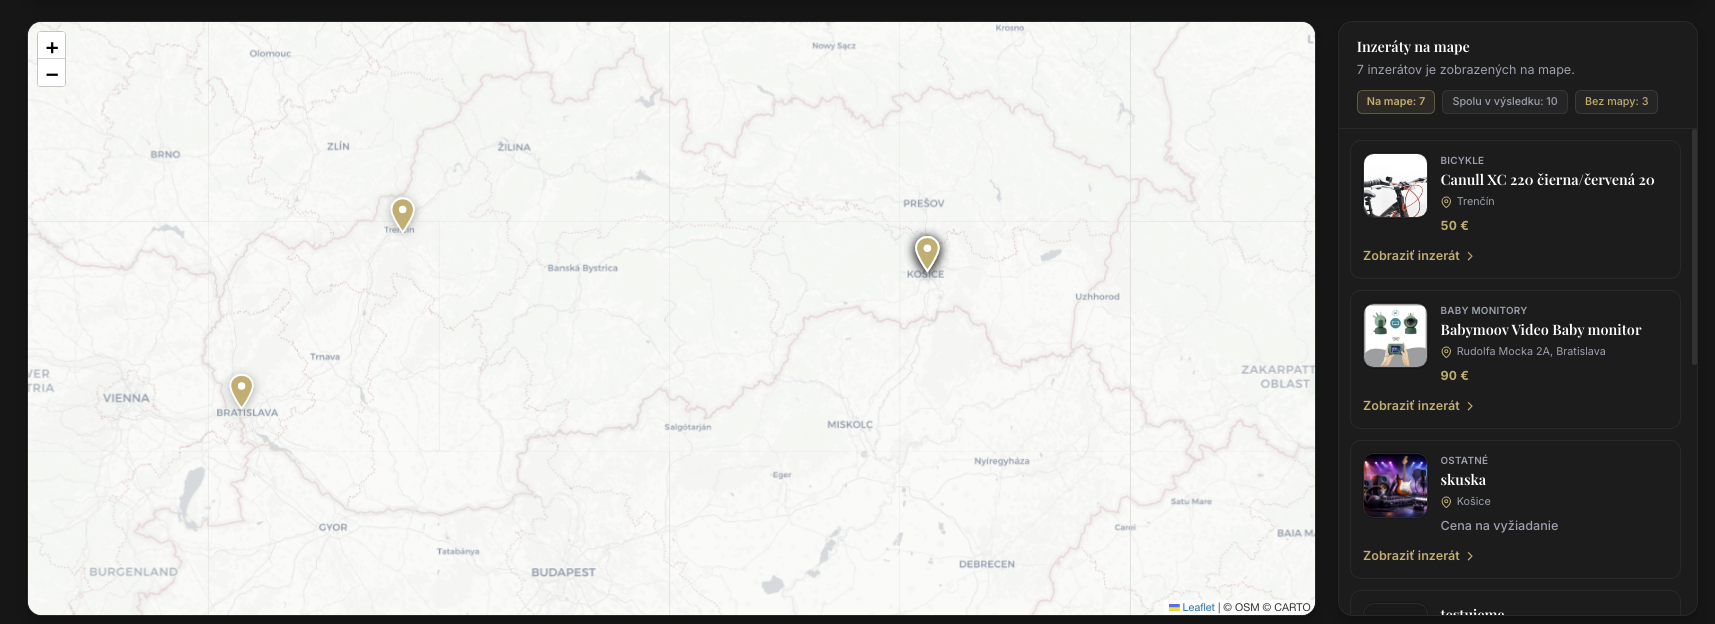
\includegraphics[width=\textwidth]{images/mapa_2.png}
\caption{Interaktívny popup nad markerom v mape Leaflet -- náhľad inzerátu s fotografiou, názvom, cenou a odkazom na detail}
\label{fig:mapa-2}
\end{figure}

\subsection{Perzistencia dát: PostgreSQL a Prisma ORM}
\noindent
Efektívna správa dát je základom každej úspešnej webovej aplikácie. V mojom projekte som sa rozhodol pre technologický zásobník, ktorý zaručuje integritu údajov, vysoký výkon pri zložitých dopytoch a vynikajúcu skúsenosť pri vývoji v TypeScripte.

\subsubsection{Relačná databáza PostgreSQL}
\noindent
Ako úložisko dát som zvolil PostgreSQL, čo je pokročilá open-source objektovo-relačná databáza \parencite{obe2017postgresql}.

\begin{itemize}
  \item \textbf{Spoľahlivosť a integrita:} PostgreSQL striktne dodržiava princípy ACID (\emph{Atomicity}, \emph{Consistency}, \emph{Isolation}, \emph{Durability}) \parencite{obe2017postgresql}, čo je nevyhnutné pri operáciách, ako je registrácia používateľa alebo spracovanie správ, kde nesmie dôjsť k strate či poškodeniu dát.
  \item \textbf{Podpora geografických dát:} Vzhľadom na to, že platforma využíva mapové podklady, PostgreSQL je ideálnou voľbou vďaka svojej schopnosti efektívne pracovať so súradnicami a priestorovými dopytmi.
  \item \textbf{Výkon pri vyhľadávaní:} Databáza umožňuje vytvárať indexy nad kľúčovými poľami (napr.\ \hlcode{userId}, \hlcode{status}, \hlcode{categoryId} či \hlcode{createdAt} v entite \hlcode{Advertisement}, alebo \hlcode{slug} v entite \hlcode{Category}), čo zabezpečuje bleskovú odozvu pri filtrovaní tisícok inzerátov.
  \item \textbf{Flexibilita s JSONB:} Využitie typu JSONB v PostgreSQL mi umožňuje ukladať dynamické parametre inzerátov (špecifikácie) s vysokým výkonom, pričom nad týmito dátami je možné vykonávať efektívne dopyty takmer rovnako rýchlo ako nad klasickými stĺpcami.
\end{itemize}

\subsubsection{Prisma ORM (Object-Relational Mapping)}
\noindent
Na komunikáciu medzi NestJS backendom a databázou PostgreSQL využívam Prisma ORM \parencite{winters2020swe}. Na rozdiel od tradičných ORM nástrojov, Prisma funguje na báze deklaratívnej schémy, ktorá slúži ako jediný zdroj pravdy (\emph{Single Source of Truth}) pre celý projekt.

\begin{itemize}
  \item \textbf{Typová bezpečnosť (\emph{Type-safety}):} Prisma automaticky generuje TypeScript klient na základe definovanej schémy (\hlcode{schema.prisma}). Výsledný klient je dostupný ako npm balík v priečinku \hlcode{node\_modules}. Vďaka tomu vývojové prostredie (napr.\ VS~Code) presne vie, aké polia má napríklad model \hlcode{User}, bez nutnosti ručného písania TypeScript rozhraní pre databázu. Pri písaní databázových dopytov je k dispozícii kompletné automatické dopĺňanie kódu a kompilátor upozorní na akúkoľvek nezrovnalosť.
  \item \textbf{Prisma Schema:} V tomto súbore definujem nielen tabuľky (modely), ale aj ich vzájomné vzťahy (napr. \texttt{@relation} medzi inzerátom a autorom) a enumerátory (\texttt{enum}) pre stavy inzerátov či roly používateľov.
  \item \textbf{Migrácie (Prisma Migrate):} Každú zmenu v štruktúre databázy spravujem pomocou migrácií. Prisma sleduje históriu zmien a umožňuje ich bezpečné a reprodukovateľné nasadenie na produkčný server, čím sa eliminuje riziko manuálnych chýb pri správe SQL skriptov.
  \item \textbf{Výkon a optimalizácia (SQL vs.\ ORM):} Hoci použitie ORM môže v porovnaní s čistým SQL priniesť mierny režijný náklad (\emph{overhead}), Prisma je vysoko optimalizovaná a generuje efektívne SQL dopyty. Tento minimálny rozdiel vo výkone je bohato kompenzovaný elimináciou ľudských chýb pri písaní dopytov a obrovským zrýchlením vývoja vďaka typovej bezpečnosti.
\end{itemize}

\subsubsection{Prospech pre Monorepo architektúru}
\noindent
V rámci monorepa je Prisma umiestnená v samostatnom balíku \hlcode{packages/database}. Tento prístup umožňuje:

\begin{itemize}
  \item \textbf{Zdieľanie schémy:} API aplikácia využíva vygenerovaný klient na zápis a čítanie dát, zatiaľ čo ostatné časti projektu môžu využívať vygenerované typy pre validáciu.
  \item \textbf{Jednoduchá údržba:} Ak potrebujem pridať nové pole do inzerátu (napríklad „vratná kaucia“), zmením to na jednom mieste v schéme, spustím migráciu a zmena sa okamžite prejaví v celom vývojovom prostredí.
\end{itemize}

\subsection{Voľba technológií: Node.js ekosystém verzus PHP}
\noindent
Pri rozhodovaní o technologickom zásobníku som zvažoval dve hlavné alternatívy: klasický prístup postavený na PHP (napríklad frameworky Laravel alebo Symfony) a moderný prístup postavený na Node.js s TypeScriptom (NestJS na backende, Next.js na frontende). Táto kapitola popisuje dôvody, prečo som sa rozhodol pre druhú možnosť.

\subsubsection{Asynchrónny model spracovania požiadaviek}
\noindent
PHP tradične funguje na modeli \emph{one-process-per-request}: každá HTTP požiadavka spustí nový PHP proces (alebo vlákno), ktorý blokuje výpočtové zdroje počas celého trvania operácie. Pri paralelnom prístupe tisícov používateľov to vedie k výraznému zaťaženiu servera.

Node.js naproti tomu využíva \emph{event loop} -- neblokujúci, jednovláknový model. Asynchrónne I/O operácie (databázové dopyty, čítanie súborov) sa vykonávajú na pozadí a vlákno sa uvoľní pre ďalšie požiadavky okamžite po spustení operácie. Pre inzertný portál, kde dominujú I/O operácie (čítanie inzerátov z databázy, odosielanie správ), je tento model ideálny a umožňuje obsluhovať oveľa väčší počet súbežných požiadaviek s nižšími hardvérovými nárokmi \parencite{casciaro2020nodejs}.

\subsubsection{Jednotný jazyk naprieč celým stackom}
\noindent
Jednou z najvýznamnejších výhod zvoleného riešenia je použitie jediného jazyka -- TypeScriptu -- na backende aj frontende. PHP je výhradne serverový jazyk; frontend musí byť napísaný oddelene v JavaScripte. Výsledkom sú dve nezávislé kódové základne, ktoré si nemôžu zdieľať typy ani validačnú logiku.

V mojom monorepe je balík \hlcode{packages/shared} zdieľaný medzi NestJS API a všetkými troma Next.js aplikáciami. Ak zmením štruktúru DTO pre inzerát, TypeScript kompilátor okamžite upozorní na nezrovnalosti na všetkých miestach -- na backende aj frontende -- ešte pred spustením aplikácie. Tento mechanizmus \emph{end-to-end} typovej bezpečnosti \parencite{cherny2019typescript} prakticky eliminuje celú kategóriu chýb spôsobených nekonzistentnými dátovými typmi, ktoré sú v PHP/JavaScript projektoch bežné.

\subsubsection{Server-Side Rendering a SEO}
\noindent
V PHP je generovanie HTML na serveri prirodzenou súčasťou jazyka (šablóny Blade, Twig, Latte). Avšak moderné PHP aplikácie stále čoraz viac spoliehajú na JavaScript SPA (Single Page Application), čím strácajú výhodu natívneho SSR a vyžadujú komplexné konfigurácie na zachovanie SEO.

Next.js prináša to najlepšie z oboch svetov: React Server Components generujú HTML priamo na serveri (rovnako ako PHP), zatiaľ čo interaktívne časti stránky sú hydratované v prehliadači. Pre inzertný portál je toto kritické -- vyhľadávače ako Google musia vedieť indexovať obsah inzerátov okamžite z HTML, bez nutnosti spúšťania JavaScriptu. Zároveň Next.js automaticky optimalizuje obrázky, fonty a skriptové súbory, čo by v PHP vyžadovalo manuálnu konfiguráciu ďalších nástrojov \parencite{riva2022nextjs}.

\subsubsection{Ekosystém, nástroje a Developer Experience}
\noindent
PHP ekosystém (Composer, PHPUnit, Eloquent ORM) je síce zrelý a stabilný, avšak npm ekosystém je oveľa rozsiahlejší. Pre kľúčové komponenty mojej platformy -- interaktívne mapy (Leaflet), vizuálny editor obsahu (GrapesJS), real-time chat -- existujú natívne npm balíky s aktuálnou podporou. Integrácia rovnakých knižníc do PHP backendu by si vyžiadala ich použitie len na frontende, čo zvyšuje komplexitu projektovej štruktúry.

Prisma ORM pre Node.js poskytuje typovo bezpečné databázové dopyty s autokompletizáciou v IDE, ktorá nemá priamu obdobu v PHP. Eloquent ORM v Laraveli je síce elegantný, ale neposkytuje kompilačnú typovú bezpečnosť; chyby v databázových dopytoch sa prejavia až pri behu aplikácie.

\subsubsection{Zhrnutie porovnania}
\noindent
Tabuľka~\ref{tab:php-vs-node} sumarizuje kľúčové rozdiely medzi oboma prístupmi z pohľadu požiadaviek tohto projektu.

\begin{table}[htbp]
\centering
\begingroup
\footnotesize
\setlength{\tabcolsep}{6pt}
\renewcommand{\arraystretch}{1.35}
\rowcolors{2}{gray!7}{white}
\begin{tabular}{@{}>{\raggedright\arraybackslash}p{0.26\linewidth}>{\raggedright\arraybackslash}p{0.32\linewidth}>{\raggedright\arraybackslash}p{0.32\linewidth}@{}}
\toprule
\rowcolor{gray!14}
\textbf{Kritérium} & \textbf{PHP (Laravel)} & \textbf{Node.js / TypeScript} \\
\midrule
Model požiadaviek & Blokujúci (process-per-request) & Neblokujúci (event loop) \\
Zdieľanie typov & Nie (2 jazyky) & Áno (monorepo, TS) \\
SSR + SEO & Šablónový engine alebo SPA+konfigurácia & Natívne (Next.js RSC) \\
Typová bezpečnosť & Čiastočná (PHP 8+) & Kompletná (TypeScript) \\
ORM & Eloquent (runtime chyby) & Prisma (compile-time) \\
Mapové knižnice & JS knižnice cez npm (frontend only) & Priama integrácia (React) \\
Nasadenie & Apache/Nginx + PHP-FPM & Node.js / Docker / Vercel \\
\bottomrule
\end{tabular}
\endgroup
\caption{Porovnanie PHP (Laravel) a Node.js/TypeScript ekosystému}
\label{tab:php-vs-node}
\end{table}

\noindent
Na základe tohto porovnania je zrejmé, že pre projekt s troma frontendovými aplikáciami, zdieľanými typmi a požiadavkou na SSR je Node.js/TypeScript stack výrazne vhodnejší ako tradičné PHP riešenie.

\subsection{Nástroje pre správu kódu a kontajnerizáciu (Git, Docker Compose)}
\noindent
Efektívny vývoj softvéru vyžaduje nielen kvalitný kód, ale aj spoľahlivé nástroje na jeho verzovanie a orchestráciu služieb. V mojom projekte hrajú kľúčovú úlohu systémy Git a Docker, ktoré umožňujú bezpečnú správu verzií a izoláciu behového prostredia.

\subsubsection{Verzovanie kódu pomocou systému Git}
\noindent
Systém Git je základným nástrojom na sledovanie zmien v zdrojovom kóde \parencite{winters2020swe}. V kontexte monorepa je jeho dôležitosť ešte vyššia, nakoľko spravuje históriu viacerých aplikácií a zdieľaných balíkov súčasne.

\begin{itemize}
  \item \textbf{Vetvenie (\emph{Branching strategy}):} Vývoj prebieha primárne na hlavnej vetve (\hlcode{main}), pričom Git umožňuje pri väčších zmenách vytvárať samostatné vetvy pre jednotlivé funkcie (napr.\ \hlcode{feature/auth} pre autentifikáciu alebo \hlcode{feature/map-logic} pre mapovú logiku), čo umožňuje experimentovať s novými funkciami bez rizika narušenia stability hlavnej vetvy.
  \item \textbf{História a audit:} Git uchováva detailný prehľad o tom, kedy a prečo bola konkrétna zmena vykonaná. To je kľúčové pri hľadaní chýb (\emph{debugging}) alebo pri návrate k predchádzajúcej stabilnej verzii aplikácie.
  \item \textbf{Ignorovanie súborov (\hlcode{.gitignore}):} Pomocou tohto súboru zabezpečujem, že sa do repozitára nedostanú zbytočné dáta (napríklad vygenerované priečinky \hlcode{node\_modules}) alebo citlivé údaje (ako sú konfiguračné súbory \hlcode{.env}).
\end{itemize}

\subsubsection{Kontajnerizácia pomocou technológie Docker}
\noindent
Pre zabezpečenie konzistentného správania aplikácie som sa rozhodol pre Docker \parencite{winters2020swe}. Táto technológia umožňuje „zabaliť” aplikáciu spolu so všetkými jej závislosťami (Node.js, knižnice, konfiguračné súbory) do izolovaného kontajnera.

\begin{itemize}
  \item \textbf{Docker Image:} Každá časť systému (API, frontendy) má definovaný svoj vlastný \hlcode{Dockerfile}. Ten obsahuje inštrukcie na zostavenie obrazu, čím sa eliminuje problém typu „u mňa v počítači to funguje“, pretože kontajner beží v identickom prostredí bez ohľadu na operačný systém hostiteľa.
  \item \textbf{Izolácia databázy:} Docker využívam aj na spustenie databázy PostgreSQL. Vďaka tomu nemusím databázový server inštalovať priamo do operačného systému, čo udržuje vývojové prostredie čisté a ľahko prenosné.
\end{itemize}

\subsubsection{Orchestrácia služieb cez Docker Compose}
\noindent
Vzhľadom na to, že môj projekt pozostáva z viacerých súbežne bežiacich služieb (API, tri frontendy a databáza), využívam nástroj Docker Compose.

\begin{itemize}
  \item \textbf{Konfigurácia jedným súborom:} Súbor \hlcode{docker-compose.yml} definuje celý ekosystém aplikácie. Obsahuje informácie o portoch, prepojeniach medzi kontajnermi a premenných prostredia.
  \item \textbf{Jednoduchosť spustenia:} Celé komplexné prostredie je možné uviesť do prevádzky jediným príkazom \hlcode{docker-compose up}. Tento prístup dramaticky zrýchľuje proces nasadenia (\emph{deployment}) a uľahčuje spoluprácu, ak by sa na projekte podieľalo viacero vývojárov.
  \item \textbf{Bezpečnosť a siete (\emph{Networking}):} Vďaka Docker Compose sú služby ako API a databáza prepojené v spoločnej internej virtuálnej sieti. To zvyšuje bezpečnosť, pretože databázový port nemusí byť vystavený do verejného internetu, ale je prístupný výhradne pre backendovú aplikáciu.
\end{itemize}

\subsubsection{Prepojenie s monorepom a optimalizácia obrazov}
\noindent
Nástroje na správu kódu sú plne integrované s \hlcode{npm workspaces}. Pri vytváraní Docker obrazov využívam viacúrovňové zostavovanie (\emph{multi-stage builds}). V prvej fáze (\emph{build stage}) sa nainštalujú všetky vývojárske závislosti a TypeScript kód sa skompiluje. V druhej fáze (\emph{production stage}) sa do výsledného obrazu prekopíruje už len hotový JavaScript a produkčné knižnice (vrátane nevyhnutných súborov zo zdieľaných balíkov \hlcode{packages/}).

Výsledný kontajner je tak o stovky megabajtov menší a neobsahuje pôvodný zdrojový kód, čo sťažuje prípadný útok. K bezpečnosti a optimalizácii veľkosti prispieva aj súbor \hlcode{.dockerignore}, ktorý zabraňuje prekopírovaniu zbytočností (ako lokálne \hlcode{node\_modules}) či citlivých dát (\hlcode{.env} súbory) do vnútra kontajnera pri jeho zostavovaní.

\section{Realizácia a implementácia systému}
\noindent
Implementácia systému prebiehala v súlade s princípmi moderného full-stack vývoja. V tejto kapitole detailne rozoberám vnútornú štruktúru projektu, spôsob zdieľania kódu a konkrétne technické riešenia jednotlivých modulov.

\subsection{Štruktúra monorepa a zdieľanie typov}
\noindent
Pre správu celého ekosystému som zvolil architektúru monorepa s využitím nástroja \emph{npm workspaces} \parencite{winters2020swe}. Tento prístup mi umožnil sústrediť frontendovú aj backendovú logiku do jedného úložiska, čo výrazne zjednodušilo refaktoring a správu závislostí.

\subsubsection{Organizácia adresárovej štruktúry}
\noindent
Projekt je rozdelený do dvoch hlavných priečinkov, ktoré jasne oddeľujú spustiteľné aplikácie od knižníc. Pre lepšiu orientáciu uvádzam zjednodušenú štruktúru projektu:

\begin{lstlisting}[
  basicstyle=\scriptsize\ttfamily\color{vscText},
  backgroundcolor=\color{vscBg},
  frame=single,
  framesep=6pt,
  framerule=0.3pt,
  rulecolor=\color{vscFrame},
  xleftmargin=8pt,
  xrightmargin=4pt,
  aboveskip=6pt,
  belowskip=6pt,
]
.
|-- apps/
|   |-- admin/        # Next.js (Admin panel)
|   |-- api/          # NestJS (Backend)
|   |-- platform/     # Next.js (Verejny web)
|   `-- user/         # Next.js (Pouzivatelska zona)
|-- packages/
|   |-- database/     # Prisma schema a klient
|   `-- shared/       # DTOs, TypeScript typy
|-- package.json      # npm workspaces
`-- docker-compose.yml
\end{lstlisting}
\vspace{0.35\baselineskip}

\begin{itemize}
  \item \textbf{\texttt{apps/}:} Obsahuje štyri samostatné projekty: \hlcode{api} (NestJS), \hlcode{platform} (verejný Next.js web), \hlcode{user} (používateľská zóna) a \hlcode{admin} (správcovský panel). Každá z týchto aplikácií má vlastnú konfiguráciu a beží na samostatnom porte.
  \item \textbf{\texttt{packages/}:} Obsahuje zdieľané moduly, ktoré nie sú samostatne spustiteľné, ale poskytujú logiku pre ostatné aplikácie. Najdôležitejšími sú \hlcode{database} (Prisma schéma a klient) a \hlcode{shared} (spoločné typy).
\end{itemize}

\subsubsection{Implementácia \texttt{packages/shared} a zdieľanie typov}
\noindent
Jednou z najväčších výziev pri vývoji oddeleného frontendu a backendu je udržanie konzistentných dátových typov. V mojom projekte som tento problém vyriešil vytvorením balíka \hlcode{shared}, ktorý slúži ako „jediný zdroj pravdy“.

\begin{itemize}
  \item \textbf{Zdieľané rozhrania (\emph{Interfaces}):} V tomto balíku definujem štruktúru všetkých objektov, ktoré prechádzajú cez sieť. Ak napríklad definujem rozhranie \hlcode{IAdvertisement}, obe strany (API aj frontend) presne vedia, aké polia má daný objekt obsahovať (napr.\ \hlcode{title}, \hlcode{price}, \hlcode{images}).
  \item \textbf{DTO (\emph{Data Transfer Objects}):} Pomocou knižnice \hlcode{class-validator} definujem v tomto balíku aj pravidlá pre validáciu vstupov. Tieto DTO triedy využíva NestJS na kontrolu prichádzajúcich požiadaviek a zároveň ich Next.js využíva na definovanie typov vo formulároch. Je dôležité zdôrazniť rozdelenie zodpovednosti: kým TypeScript stráži typy počas vývoja (\emph{compile-time}), \hlcode{class-validator} stráži dáta počas behu aplikácie (\emph{runtime}) a overuje napríklad to, či je zadaný textový reťazec skutočne platným e-mailom.
  \item \textbf{End-to-End bezpečnosť:} Vďaka tomuto prepojeniu ma kompilátor TypeScriptu okamžite upozorní, ak na backende zmením názov poľa v databáze, ale na frontende sa ho stále pokúšam zobraziť. Týmto spôsobom som eliminoval veľké množstvo chýb, ktoré bežne vznikajú pri manuálnom prepisovaní typov.
\end{itemize}

\subsubsection{Mechanizmus npm workspaces}
\noindent
Nástroj \emph{npm workspaces} zabezpečuje, že všetky balíky v rámci monorepa sú navzájom prepojené prostredníctvom symbolických odkazov (\emph{symlinks}). To znamená, že pri lokálnom vývoji nemusím balík \hlcode{shared} zakaždým publikovať; zmeny vykonané v zdieľanom kóde sa okamžite prejavia vo všetkých aplikáciách, ktoré ho importujú. Tento mechanizmus je kľúčový pre agilný vývoj a rýchle prototypovanie nových funkcií.

Okrem toho \emph{npm workspaces} rieši problém s duplicitnými závislosťami (tzv.\ \emph{hoisting}). Všetky aplikácie zdieľajú jeden spoločný priečinok \hlcode{node\_modules} v koreni projektu, čo výrazne šetrí miesto na disku a zrýchľuje inštaláciu závislostí.

\subsection{Realizácia backendových modulov}
\noindent
Každý modul v systéme pozostáva z troch základných vrstiev: \emph{Controller} (vstupná brána a definícia endpointov), \emph{Service} (aplikačná logika a komunikácia s databázou) a \emph{Module} (konfigurácia závislostí) \parencite{martin2017cleanarch}.

\subsubsection{Modul Auth: Autentifikácia a autorizácia}
\noindent
Tento modul je zodpovedný za bezpečnosť a správu identít. Implementácia využíva knižnicu \hlcode{@nestjs/passport} a stratégie pre JWT.

\begin{itemize}
  \item \textbf{Registrácia a login:} Služba \hlcode{AuthService} využíva bcrypt na porovnávanie hashovaných hesiel. Pri úspešnom prihlásení vygeneruje bezpečne podpísaný JWT token s exspiráciou. Payload tohto tokenu obsahuje identifikátor používateľa (\hlcode{sub}) a jeho rolu (\hlcode{role}), čo minimalizuje nutnosť dopytovať sa do databázy pri každom overovaní oprávnení.
  \item \textbf{Zabezpečenie:} Na ochranu endpointov som vytvoril globálne guardy. \hlcode{JwtAuthGuard} extrahuje token z hlavičky HTTP požiadavky a validuje ho, zatiaľ čo \hlcode{RolesGuard} v spolupráci s dekorátorom \hlcode{@Roles()} kontroluje úroveň oprávnení (napr.\ prístup k mazaniu používateľov).
\end{itemize}

\subsubsection{Modul Advertisements: Správa inzerátov a médií}
\noindent
Modul \hlcode{AdvertisementsModule} je najrozsiahlejšou časťou backendu, nakoľko spracováva hlavnú entitu systému -- inzerát.

\begin{itemize}
  \item \textbf{CRUD operácie:} Implementoval som endpointy pre vytvorenie, čítanie, aktualizáciu a mazanie inzerátov. Každý inzerát je identifikovaný unikátnym UUID, ktoré sa používa v URL detailu inzerátu a v relačných väzbách na ďalšie entity.
  \item \textbf{Spracovanie polohy:} Inzeráty ukladajú GPS súradnice (latitúda, longitúda), ktoré sú nevyhnutné pre zobrazenie na mape vo frontende.
  \item \textbf{Stavy inzerátov:} Logika v \hlcode{AdvertisementsService} zabezpečuje prechody medzi všetkými stavmi definovanými v \hlcode{AdvertisementStatus}: \hlcode{PENDING} (čakajúci na schválenie), \hlcode{DRAFT} (rozpracovaný koncept), \hlcode{ACTIVE} (viditeľný), \hlcode{INACTIVE} (deaktivovaný používateľom) a \hlcode{ARCHIVED} (archivovaný). Úplnú mapu prechodov medzi týmito stavmi vrátane aktérov, ktorí jednotlivé akcie vyvolávajú (používateľ vs.\ administrátor), zobrazuje obrázok~\ref{fig:state-advertisement}.
\end{itemize}

\begin{figure}[htbp]
\centering
\resizebox{!}{0.65\textheight}{% State diagram životného cyklu inzerátu (AdvertisementStatus)
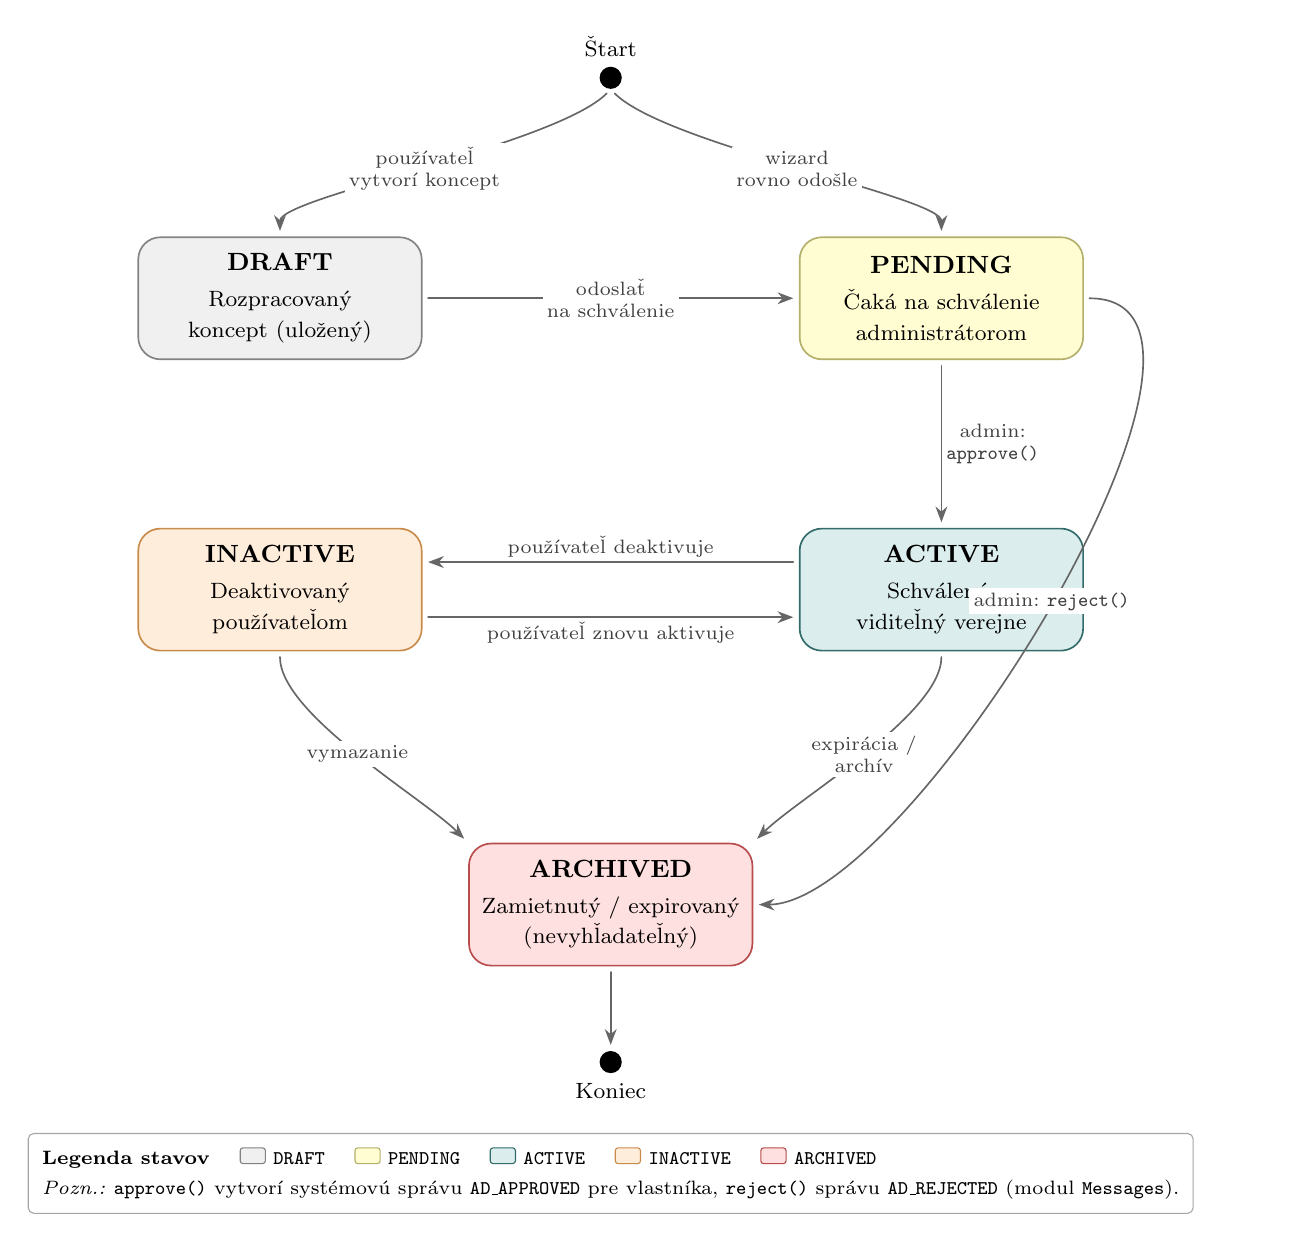
\begin{tikzpicture}[
  font=\rmfamily\small,
  line cap=round, line join=round,
  >=Stealth,
  state/.style={
    rectangle, rounded corners=8pt,
    minimum width=3.6cm, minimum height=1.55cm,
    align=center, inner sep=4pt,
    line width=0.6pt,
    font=\rmfamily\small
  },
  draftst/.style={state, draw=gray!60!black!70, fill=gray!12!white},
  pendingst/.style={state, draw=yellow!55!black!75, fill=yellow!18!white},
  activest/.style={state, draw=teal!55!black!80, fill=teal!14!white},
  inactivest/.style={state, draw=orange!70!black!70, fill=orange!14!white},
  archivedst/.style={state, draw=red!60!black!70, fill=red!12!white},
  startend/.style={circle, fill=black, inner sep=2pt, minimum size=8pt},
  trans/.style={->, line width=0.6pt, draw=black!60, shorten >=2pt, shorten <=2pt},
  edgelbl/.style={font=\rmfamily\scriptsize, fill=white, inner sep=1.5pt, text=black!75, align=center}
]

% =========================================================================
% Layout (vertikálny portrait, široký 14 cm)
% =========================================================================

% Štart
\node[startend, label={[font=\rmfamily\footnotesize]above:Štart}] (start) at (0, 0) {};

% Riadok 1: DRAFT (vľavo) a PENDING (vpravo)
\node[draftst]   (draft)   at (-4.2, -2.8) {%
  \textbf{DRAFT}\\[2pt]
  \footnotesize Rozpracovaný\\
  \footnotesize koncept (uložený)
};

\node[pendingst] (pending) at ( 4.2, -2.8) {%
  \textbf{PENDING}\\[2pt]
  \footnotesize Čaká na schválenie\\
  \footnotesize administrátorom
};

% Riadok 2: INACTIVE (vľavo) a ACTIVE (vpravo)
\node[inactivest] (inactive) at (-4.2, -6.5) {%
  \textbf{INACTIVE}\\[2pt]
  \footnotesize Deaktivovaný\\
  \footnotesize používateľom
};

\node[activest]   (active)   at ( 4.2, -6.5) {%
  \textbf{ACTIVE}\\[2pt]
  \footnotesize Schválený,\\
  \footnotesize viditeľný verejne
};

% Riadok 3: ARCHIVED (stred)
\node[archivedst] (archived) at (0, -10.5) {%
  \textbf{ARCHIVED}\\[2pt]
  \footnotesize Zamietnutý / expirovaný\\
  \footnotesize (nevyhľadateľný)
};

% Koncový stav
\node[startend, label={[font=\rmfamily\footnotesize]below:Koniec}] (end) at (0, -12.5) {};

% =========================================================================
% Prechody
% =========================================================================
% Štart -> DRAFT
\draw[trans] (start.south) .. controls +(south west:1.0) and +(north:0.5) ..
  node[edgelbl, pos=0.5] {používateľ\\ vytvorí koncept} (draft.north);

% Štart -> PENDING
\draw[trans] (start.south) .. controls +(south east:1.0) and +(north:0.5) ..
  node[edgelbl, pos=0.5] {wizard\\ rovno odošle} (pending.north);

% DRAFT -> PENDING
\draw[trans] (draft.east) -- node[edgelbl, pos=0.5] {odoslať\\ na schválenie} (pending.west);

% PENDING -> ACTIVE
\draw[trans] (pending.south) -- node[edgelbl, pos=0.5, right] {admin:\\ \texttt{approve()}} (active.north);

% PENDING -> ARCHIVED (oblúk vpravo)
\draw[trans] (pending.east) .. controls +(east:2.5) and +(east:2.0) ..
  node[edgelbl, pos=0.5] {admin: \texttt{reject()}} (archived.east);

% ACTIVE <-> INACTIVE (dva paralelné šípy)
\draw[trans] ($(active.west)+(0,0.35)$) -- node[edgelbl, pos=0.5, above] {používateľ deaktivuje} ($(inactive.east)+(0,0.35)$);
\draw[trans] ($(inactive.east)+(0,-0.35)$) -- node[edgelbl, pos=0.5, below] {používateľ znovu aktivuje} ($(active.west)+(0,-0.35)$);

% ACTIVE -> ARCHIVED
\draw[trans] (active.south) .. controls +(south:0.8) and +(north east:0.8) ..
  node[edgelbl, pos=0.5] {expirácia /\\ archív} (archived.north east);

% INACTIVE -> ARCHIVED
\draw[trans] (inactive.south) .. controls +(south:0.8) and +(north west:0.8) ..
  node[edgelbl, pos=0.5] {vymazanie} (archived.north west);

% ARCHIVED -> Koniec
\draw[trans] (archived.south) -- (end.north);

% =========================================================================
% Legenda dolu (centered pod end)
% =========================================================================
\node[draw=black!35, fill=white, rounded corners=2pt, inner sep=5pt,
      font=\rmfamily\scriptsize, align=left, anchor=north]
  at (0, -13.4)
{%
  \textbf{Legenda stavov} \quad
  \tikz\draw[fill=gray!12!white, draw=gray!60!black!70, line width=0.4pt, rounded corners=1pt] (0,0) rectangle (0.32,0.2); \texttt{DRAFT} \quad
  \tikz\draw[fill=yellow!18!white, draw=yellow!55!black!75, line width=0.4pt, rounded corners=1pt] (0,0) rectangle (0.32,0.2); \texttt{PENDING} \quad
  \tikz\draw[fill=teal!14!white, draw=teal!55!black!80, line width=0.4pt, rounded corners=1pt] (0,0) rectangle (0.32,0.2); \texttt{ACTIVE} \quad
  \tikz\draw[fill=orange!14!white, draw=orange!70!black!70, line width=0.4pt, rounded corners=1pt] (0,0) rectangle (0.32,0.2); \texttt{INACTIVE} \quad
  \tikz\draw[fill=red!12!white, draw=red!60!black!70, line width=0.4pt, rounded corners=1pt] (0,0) rectangle (0.32,0.2); \texttt{ARCHIVED}\\[3pt]
  \textit{Pozn.:} \texttt{approve()} vytvorí systémovú správu \texttt{AD\_APPROVED} pre vlastníka, \texttt{reject()} správu \texttt{AD\_REJECTED} (modul \texttt{Messages}).
};

\end{tikzpicture}
}
\caption{Stavový diagram životného cyklu inzerátu -- päť stavov enumerátora \texttt{AdvertisementStatus} a prechody medzi nimi; akcie vyvoláva buď používateľ (vytvorenie, odoslanie, deaktivácia) alebo administrátor (schválenie, zamietnutie)}
\label{fig:state-advertisement}
\end{figure}

\noindent\textit{Ukážka schvaľovacieho procesu inzerátu z \hlcode{AdvertisementsService}:}

\noindent\begin{minipage}{\linewidth}
\begin{lstlisting}[
  style=slovakJava,
  breakatwhitespace=true
]
async approve(id: string) {
  const advertisement = await prisma.advertisement.findUnique({ where: { id } });

  if (!advertisement) throw new NotFoundException('Inzerát nebol nájdený');
  if (advertisement.status !== 'PENDING') throw new ForbiddenException('Inzerát už bol spracovaný');

  const updated = await prisma.advertisement.update({
    where: { id },
    data: { status: 'ACTIVE' },
  });

  // systémová správa o schválení pre používateľa
  await this.messagesService.createSystemMessage(
    advertisement.userId,
    'AD_APPROVED',
    'Váš inzerát bol schválený',
    `Váš inzerát "${advertisement.title}" bol schválený a je teraz aktívny na platforme.`,
    { advertisementId: id }
  );

  return updated;
}
\end{lstlisting}
\end{minipage}
\vspace{0.4\baselineskip}
\noindent
Táto ukážka jasne demonštruje, ako je služba napísaná odolne voči chybám (využitím \hlcode{NotFoundException} a \hlcode{ForbiddenException}). Kombinuje validáciu stavu, aktualizáciu v databáze a komunikáciu s iným modulom (\hlcode{MessagesService}) pre odoslanie notifikácie používateľovi ako vedľajší efekt. Celkový tok HTTP požiadavky -- od admina, cez bezpečnostné guardy, aplikačnú službu, perzistenčnú vrstvu až po notifikáciu vlastníka inzerátu -- je vizualizovaný sekvenčným diagramom na obrázku~\ref{fig:sequence-approve}.

\begin{figure}[htbp]
\centering
\resizebox{\textwidth}{!}{% Sekvenčný diagram schválenia inzerátu - PATCH /advertisements/:id/approve
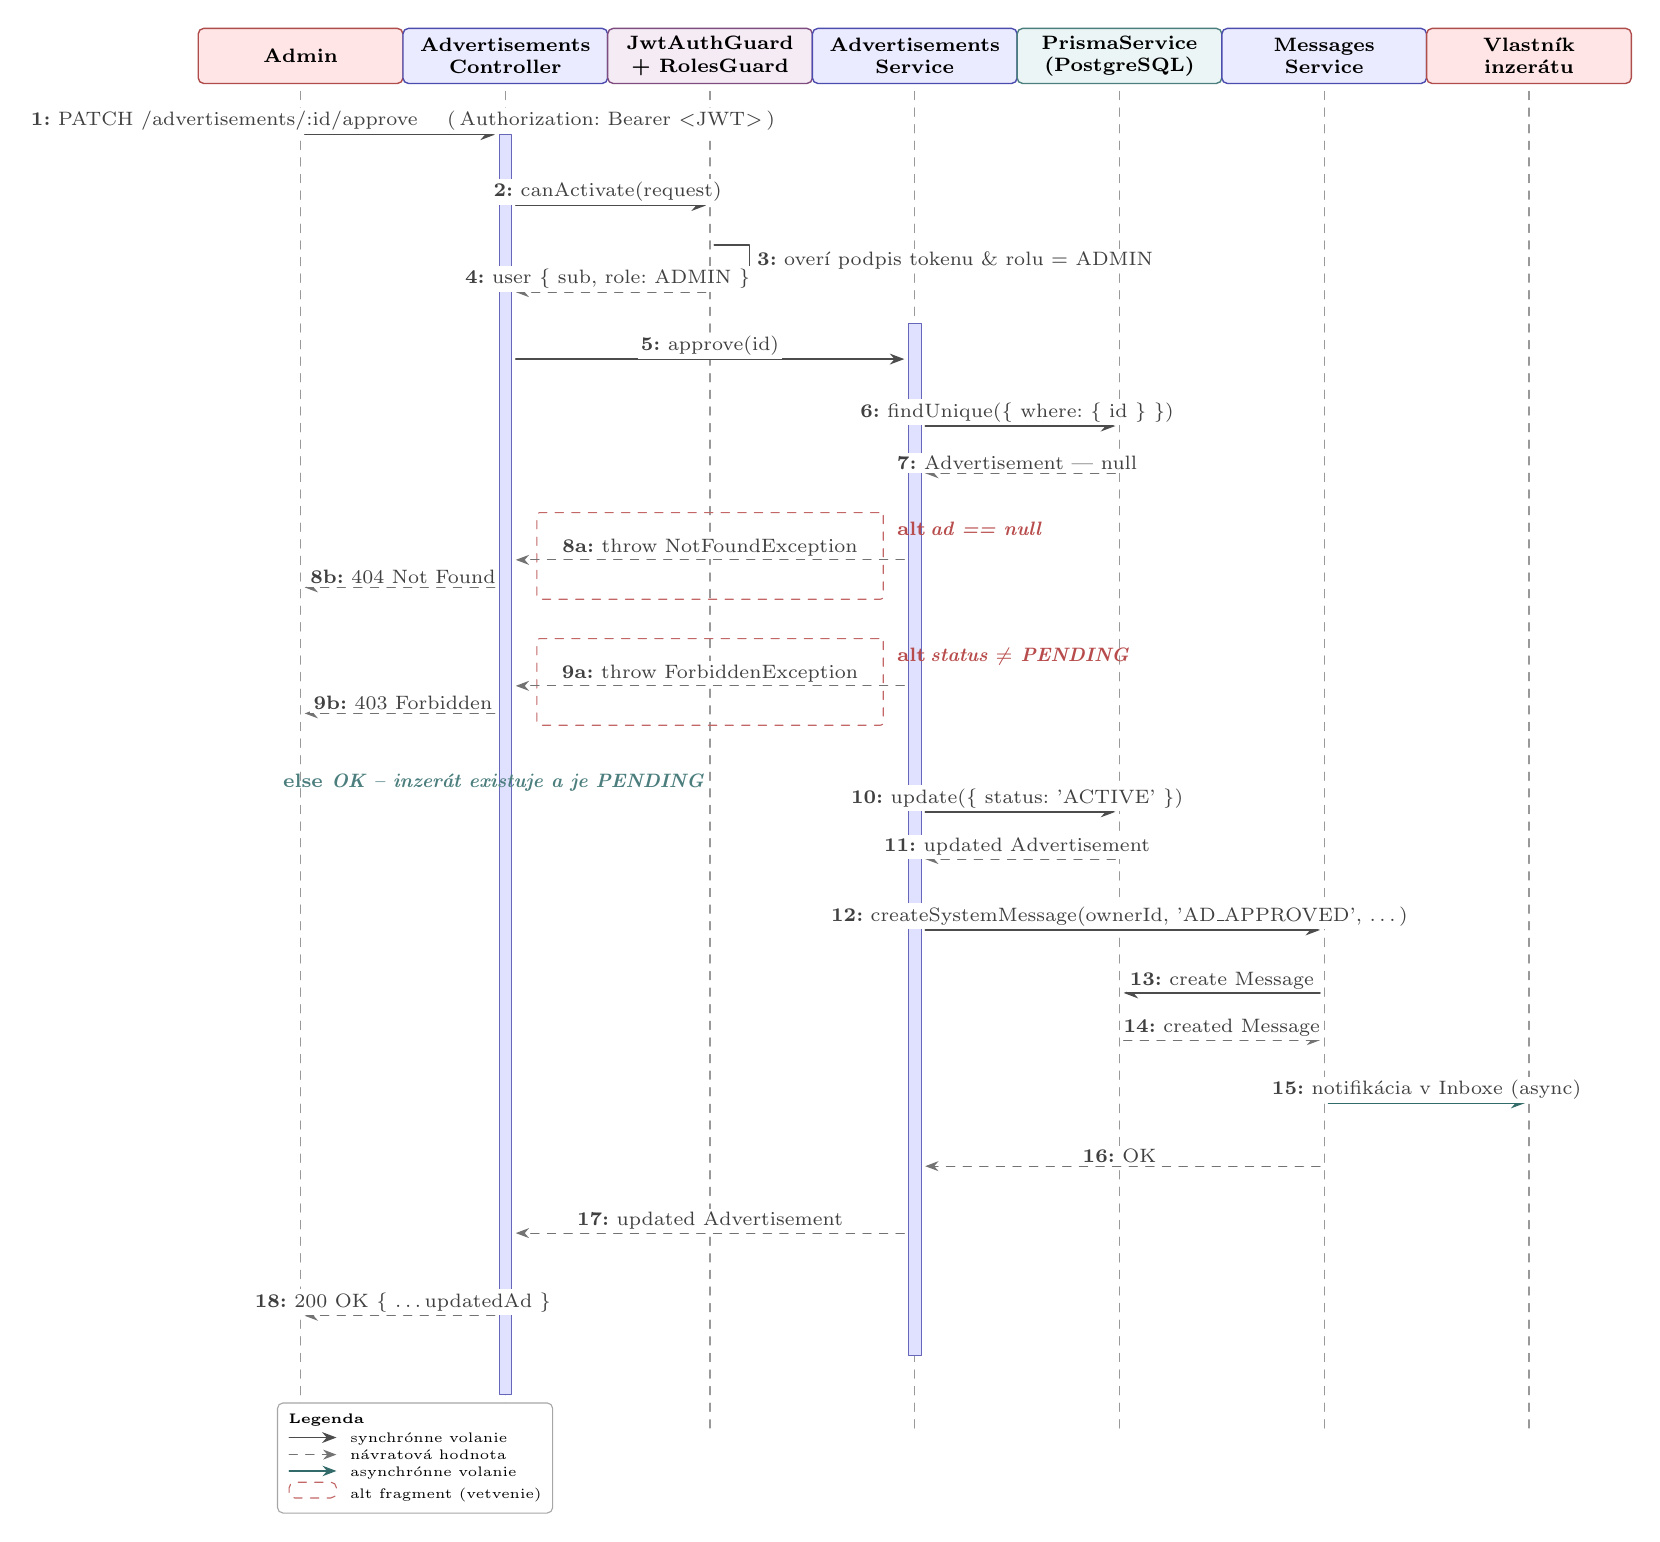
\begin{tikzpicture}[
  font=\rmfamily\scriptsize,
  line cap=round, line join=round,
  >=Stealth,
  % --- štýly ---
  lifeline/.style={line width=0.4pt, draw=black!40, dashed},
  actorhead/.style={
    rectangle, rounded corners=2pt,
    minimum width=2.6cm, minimum height=0.7cm,
    align=center, inner sep=2pt,
    line width=0.5pt,
    draw=red!55!black!70, fill=red!10!white,
    font=\rmfamily\scriptsize\bfseries
  },
  partbox/.style={
    rectangle, rounded corners=2pt,
    minimum width=2.6cm, minimum height=0.7cm,
    align=center, inner sep=2pt,
    line width=0.5pt,
    draw=blue!55!black!70, fill=blue!8!white,
    font=\rmfamily\scriptsize\bfseries
  },
  guardbox/.style={
    partbox,
    draw=violet!55!black!70, fill=violet!8!white
  },
  dbbox/.style={
    partbox,
    draw=teal!55!black!70, fill=teal!8!white
  },
  call/.style={->, line width=0.5pt, draw=black!70, shorten >=1.5pt, shorten <=1.5pt},
  retcall/.style={->, line width=0.4pt, draw=black!55, dashed, shorten >=1.5pt, shorten <=1.5pt},
  asynccall/.style={->, line width=0.45pt, draw=teal!55!black!80, shorten >=1.5pt, shorten <=1.5pt},
  msglbl/.style={font=\rmfamily\scriptsize, fill=white, inner sep=1.2pt, text=black!75, align=center},
  activation/.style={fill=blue!12!white, draw=blue!55!black!60, line width=0.3pt},
  altframe/.style={draw=red!60!black!60, line width=0.4pt, dashed, rounded corners=1pt}
]

% =========================================================================
% Lifelines (7 stĺpcov) — pozície X
% =========================================================================
\def\xA{0}        % Admin
\def\xB{2.6}      % Controller
\def\xC{5.2}      % Guard
\def\xD{7.8}      % Service
\def\xE{10.4}     % Prisma
\def\xF{13.0}     % MessagesService
\def\xG{15.6}     % Vlastník

% Hlavičky (lifeline boxes hore)
\node[actorhead] (admin)  at (\xA, 0) {Admin};
\node[partbox]   (ctrl)   at (\xB, 0) {Advertisements\\Controller};
\node[guardbox]  (guard)  at (\xC, 0) {JwtAuthGuard\\+ RolesGuard};
\node[partbox]   (svc)    at (\xD, 0) {Advertisements\\Service};
\node[dbbox]     (prisma) at (\xE, 0) {PrismaService\\(PostgreSQL)};
\node[partbox]   (msgsvc) at (\xF, 0) {Messages\\Service};
\node[actorhead] (owner)  at (\xG, 0) {Vlastník\\inzerátu};

% Lifelines (zvislé čiary)
\def\yBottom{-17.5}
\foreach \x in {\xA, \xB, \xC, \xD, \xE, \xF, \xG} {
  \draw[lifeline] (\x, -0.45) -- (\x, \yBottom);
}

% =========================================================================
% Activation bars (zvislé pruhy na lifeline) - pridáme pre ctrl a svc
% =========================================================================
\fill[activation] (\xB - 0.08, -1.0) rectangle (\xB + 0.08, -17.0);
\fill[activation] (\xD - 0.08, -3.4) rectangle (\xD + 0.08, -16.5);

% =========================================================================
% Postupnosť volaní
% =========================================================================

% 1. Admin -> Controller: PATCH
\draw[call] (\xA, -1.0) -- (\xB - 0.08, -1.0);
\node[msglbl, anchor=south] at ({(\xA+\xB)/2}, -1.0)
  {\textbf{1:} PATCH /advertisements/:id/approve \quad (\,Authorization: Bearer \textless JWT\textgreater\,)};

% 2. Controller -> Guard: canActivate
\draw[call] (\xB + 0.08, -1.9) -- (\xC, -1.9);
\node[msglbl, anchor=south] at ({(\xB+\xC)/2}, -1.9) {\textbf{2:} canActivate(request)};

% 3. Guard interne (self-loop)
\draw[call, shorten >=0pt] (\xC, -2.4) -- ++(0.5, 0) -- ++(0, -0.4) -- ++(-0.5, 0);
\node[msglbl, anchor=west] at (\xC + 0.55, -2.6) {\textbf{3:} overí podpis tokenu \& rolu = ADMIN};

% 4. Guard -> Controller: user
\draw[retcall] (\xC, -3.0) -- (\xB + 0.08, -3.0);
\node[msglbl, anchor=south] at ({(\xB+\xC)/2}, -3.0) {\textbf{4:} user \{ sub, role: ADMIN \}};

% 5. Controller -> Service: approve(id)
\draw[call] (\xB + 0.08, -3.85) -- (\xD - 0.08, -3.85);
\node[msglbl, anchor=south] at ({(\xB+\xD)/2}, -3.85) {\textbf{5:} approve(id)};

% 6. Service -> Prisma: findUnique
\draw[call] (\xD + 0.08, -4.7) -- (\xE, -4.7);
\node[msglbl, anchor=south] at ({(\xD+\xE)/2}, -4.7) {\textbf{6:} findUnique(\{ where: \{ id \} \})};

% 7. Prisma -> Service: Advertisement | null
\draw[retcall] (\xE, -5.3) -- (\xD + 0.08, -5.3);
\node[msglbl, anchor=south] at ({(\xD+\xE)/2}, -5.3) {\textbf{7:} Advertisement | null};

% alt rámec 1: ak null
\draw[altframe] (\xD - 0.4, -5.8) rectangle (\xB + 0.4, -6.9);
\node[anchor=north west, font=\rmfamily\scriptsize\bfseries, text=red!60!black!70]
  at (\xD - 0.4, -5.8) {\,alt\,\itshape ad == null\,};

\draw[retcall] (\xD - 0.08, -6.4) -- (\xB + 0.08, -6.4);
\node[msglbl, anchor=south] at ({(\xB+\xD)/2}, -6.4) {\textbf{8a:} throw NotFoundException};

\draw[retcall] (\xB - 0.08, -6.75) -- (\xA, -6.75);
\node[msglbl, anchor=south] at ({(\xA+\xB)/2}, -6.75) {\textbf{8b:} 404 Not Found};

% alt rámec 2: status != PENDING
\draw[altframe] (\xD - 0.4, -7.4) rectangle (\xB + 0.4, -8.5);
\node[anchor=north west, font=\rmfamily\scriptsize\bfseries, text=red!60!black!70]
  at (\xD - 0.4, -7.4) {\,alt\,\itshape status $\neq$ PENDING\,};

\draw[retcall] (\xD - 0.08, -8.0) -- (\xB + 0.08, -8.0);
\node[msglbl, anchor=south] at ({(\xB+\xD)/2}, -8.0) {\textbf{9a:} throw ForbiddenException};

\draw[retcall] (\xB - 0.08, -8.35) -- (\xA, -8.35);
\node[msglbl, anchor=south] at ({(\xA+\xB)/2}, -8.35) {\textbf{9b:} 403 Forbidden};

% Hlavná vetva: OK
\node[anchor=north west, font=\rmfamily\scriptsize\bfseries, text=teal!55!black!70]
  at (-0.4, -9.0) {\,else \itshape OK -- inzerát existuje a je PENDING\,};

% 10. Service -> Prisma: update
\draw[call] (\xD + 0.08, -9.6) -- (\xE, -9.6);
\node[msglbl, anchor=south] at ({(\xD+\xE)/2}, -9.6) {\textbf{10:} update(\{ status: 'ACTIVE' \})};

% 11. Prisma -> Service: updated
\draw[retcall] (\xE, -10.2) -- (\xD + 0.08, -10.2);
\node[msglbl, anchor=south] at ({(\xD+\xE)/2}, -10.2) {\textbf{11:} updated Advertisement};

% 12. Service -> MessagesService
\draw[call] (\xD + 0.08, -11.1) -- (\xF, -11.1);
\node[msglbl, anchor=south] at ({(\xD+\xF)/2}, -11.1)
  {\textbf{12:} createSystemMessage(ownerId, 'AD\_APPROVED', \dots)};

% 13. MessagesService -> Prisma: create Message
\draw[call] (\xF, -11.9) -- (\xE, -11.9);
\node[msglbl, anchor=south] at ({(\xE+\xF)/2}, -11.9) {\textbf{13:} create Message};

% 14. Prisma -> MessagesService: created Message
\draw[retcall] (\xE, -12.5) -- (\xF, -12.5);
\node[msglbl, anchor=south] at ({(\xE+\xF)/2}, -12.5) {\textbf{14:} created Message};

% 15. MessagesService -> Owner (async notifikácia)
\draw[asynccall] (\xF, -13.3) -- (\xG, -13.3);
\node[msglbl, anchor=south] at ({(\xF+\xG)/2}, -13.3) {\textbf{15:} notifikácia v Inboxe (async)};

% 16. MessagesService -> Service: OK
\draw[retcall] (\xF, -14.1) -- (\xD + 0.08, -14.1);
\node[msglbl, anchor=south] at ({(\xD+\xF)/2}, -14.1) {\textbf{16:} OK};

% 17. Service -> Controller: updated Advertisement
\draw[retcall] (\xD - 0.08, -14.95) -- (\xB + 0.08, -14.95);
\node[msglbl, anchor=south] at ({(\xB+\xD)/2}, -14.95) {\textbf{17:} updated Advertisement};

% 18. Controller -> Admin: 200 OK
\draw[retcall] (\xB - 0.08, -16.0) -- (\xA, -16.0);
\node[msglbl, anchor=south] at ({(\xA+\xB)/2}, -16.0) {\textbf{18:} 200 OK \{ \dots updatedAd \}};

% =========================================================================
% Legenda dolu (vystrihnuté zo zvyšku)
% =========================================================================
\node[draw=black!35, fill=white, rounded corners=2pt, inner sep=4pt,
      font=\rmfamily\tiny, align=left, anchor=north west]
  at (\xA - 0.3, \yBottom + 0.4)
{%
  \textbf{Legenda}\\[1pt]
  \tikz\draw[->, line width=0.5pt, draw=black!70] (0,0) -- (0.6,0); \ synchrónne volanie\\
  \tikz\draw[->, line width=0.4pt, draw=black!55, dashed] (0,0) -- (0.6,0); \ návratová hodnota\\
  \tikz\draw[->, line width=0.45pt, draw=teal!55!black!80] (0,0) -- (0.6,0); \ asynchrónne volanie\\
  \tikz\draw[draw=red!60!black!60, line width=0.4pt, dashed] (0,0) rectangle (0.6,0.2); \ alt fragment (vetvenie)
};

\end{tikzpicture}
}
\caption{Sekvenčný diagram schválenia inzerátu administrátorom -- HTTP požiadavka \texttt{PATCH /advertisements/:id/approve} postupne prechádza vrstvami \texttt{JwtAuthGuard} a \texttt{RolesGuard}, \texttt{AdvertisementsService} validuje stav inzerátu, aktualizuje záznam cez \texttt{PrismaService} a deleguje notifikáciu na \texttt{MessagesService}}
\label{fig:sequence-approve}
\end{figure}

\subsubsection{Modul Categories a dynamické filtre}
\noindent
Tento modul spravuje hierarchickú štruktúru portálu.

\begin{itemize}
  \item \textbf{Stromová štruktúra:} Kategórie podporujú rekurzívne vnorenie (Parent-Child). API vracajú stromovú štruktúru dát, ktorá sa využíva v navigačnom menu platformy.
  \item \textbf{Logika filtrov:} Každá kategória môže mať pridelenú sadu filtrov. Služba zabezpečuje, že pri vyhľadávaní v kategórii „Autá“ sa vrátia inzeráty filtrované podľa špecifických polí uložených v JSON objekte v databáze. Využívam tu schopnosť Prisma ORM dopytovať sa priamo do vnútra \hlcode{JSONB} stĺpcov, čím sa zachováva vysoký výkon vyhľadávania aj pri neštruktúrovaných dátach.
\end{itemize}

\subsubsection{Modul Search: Full-textové vyhľadávanie a analytika}
\noindent
Pre efektívne vyhľadávanie som implementoval dedikovanú logiku, ktorá kombinuje viaceré parametre.

\begin{itemize}
  \item \textbf{Filtrovanie:} Vyhľadávanie prebieha kombináciou full-textového hľadania v názve a popise inzerátu s presným filtrovaním podľa kategórie, ceny a lokality.
  \item \textbf{\hlcode{ClickEvent} integrácia:} Každé zobrazenie detailu inzerátu vyvolá asynchrónne volanie v \hlcode{AnalyticsService}, ktoré zaznamená udalosť \hlcode{ClickEvent}. Vďaka asynchrónnemu spracovaniu „na pozadí“ používateľ vôbec nečaká na zapísanie štatistiky do databázy a inzerát sa mu zobrazí okamžite. Tieto dáta sa ukladajú s informáciou o type používateľa (pohlavie, vek), čo neskôr slúži na generovanie štatistík v admin paneli.
\end{itemize}

\subsection{Vývoj klientskych aplikácií}
\noindent
Všetky tri frontendové aplikácie (\hlcode{platform}, \hlcode{user}, \hlcode{admin}) sú vybudované na rovnakom základe: Next.js App Router s React Server Components, Tailwind CSS a typmi zo zdieľaného balíka \hlcode{packages/shared}. Napriek spoločnému technologickému základu má každá aplikácia odlišný účel, vizuálnu identitu a sadu komponentov prispôsobených konkrétnej role používateľa \parencite{riva2022nextjs}.

\subsubsection{Verejná platforma (vyhľadávanie, mapa, blog)}
\noindent
Aplikácia \hlcode{apps/platform} je vstupnou bránou celej platformy a je optimalizovaná predovšetkým na rýchlosť a SEO. Väčšina stránok (zoznamy inzerátov, detail inzerátu, blog, statické stránky) je vykresľovaná ako React Server Components, čo zaručuje okamžitú odozvu a plnú indexovateľnosť obsahu vyhľadávačmi. Úvodná stránka platformy s hero sekciou, hlavnou navigáciou a prezentáciou kľúčových kategórií je zobrazená na obrázku~\ref{fig:platforma-1}.

\begin{figure}[htbp]
\centering

\includegraphics[width=\textwidth]{images/platforma_1.png}
\caption{Verejná platforma -- úvodná stránka s hero sekciou, hlavnou navigáciou a prezentáciou kľúčových kategórií}
\label{fig:platforma-1}
\end{figure}

\textbf{Vyhľadávanie a filtrovanie:} Kľúčovým prvkom je vyhľadávací panel, ktorý dynamicky načítava filtre podľa zvolenej kategórie z API. Parametre vyhľadávania sú zakódované priamo do URL adresy (\hlcode{searchParams}), čo umožňuje zdieľanie odkazu na konkrétny výsledok hľadania a zároveň zaručuje správnu indexáciu výsledkov vyhľadávačmi. Výsledná podoba prehľadu aktívnych inzerátov so zoznamovým zobrazením a postrannými filtrami je dokumentovaná na obrázku~\ref{fig:platforma-2}; obrázky~\ref{fig:category-1} a~\ref{fig:filters} ďalej zobrazujú detail kategórie s hierarchickou navigáciou a samotný panel dynamicky generovaných filtrov.

\begin{figure}[htbp]
\centering
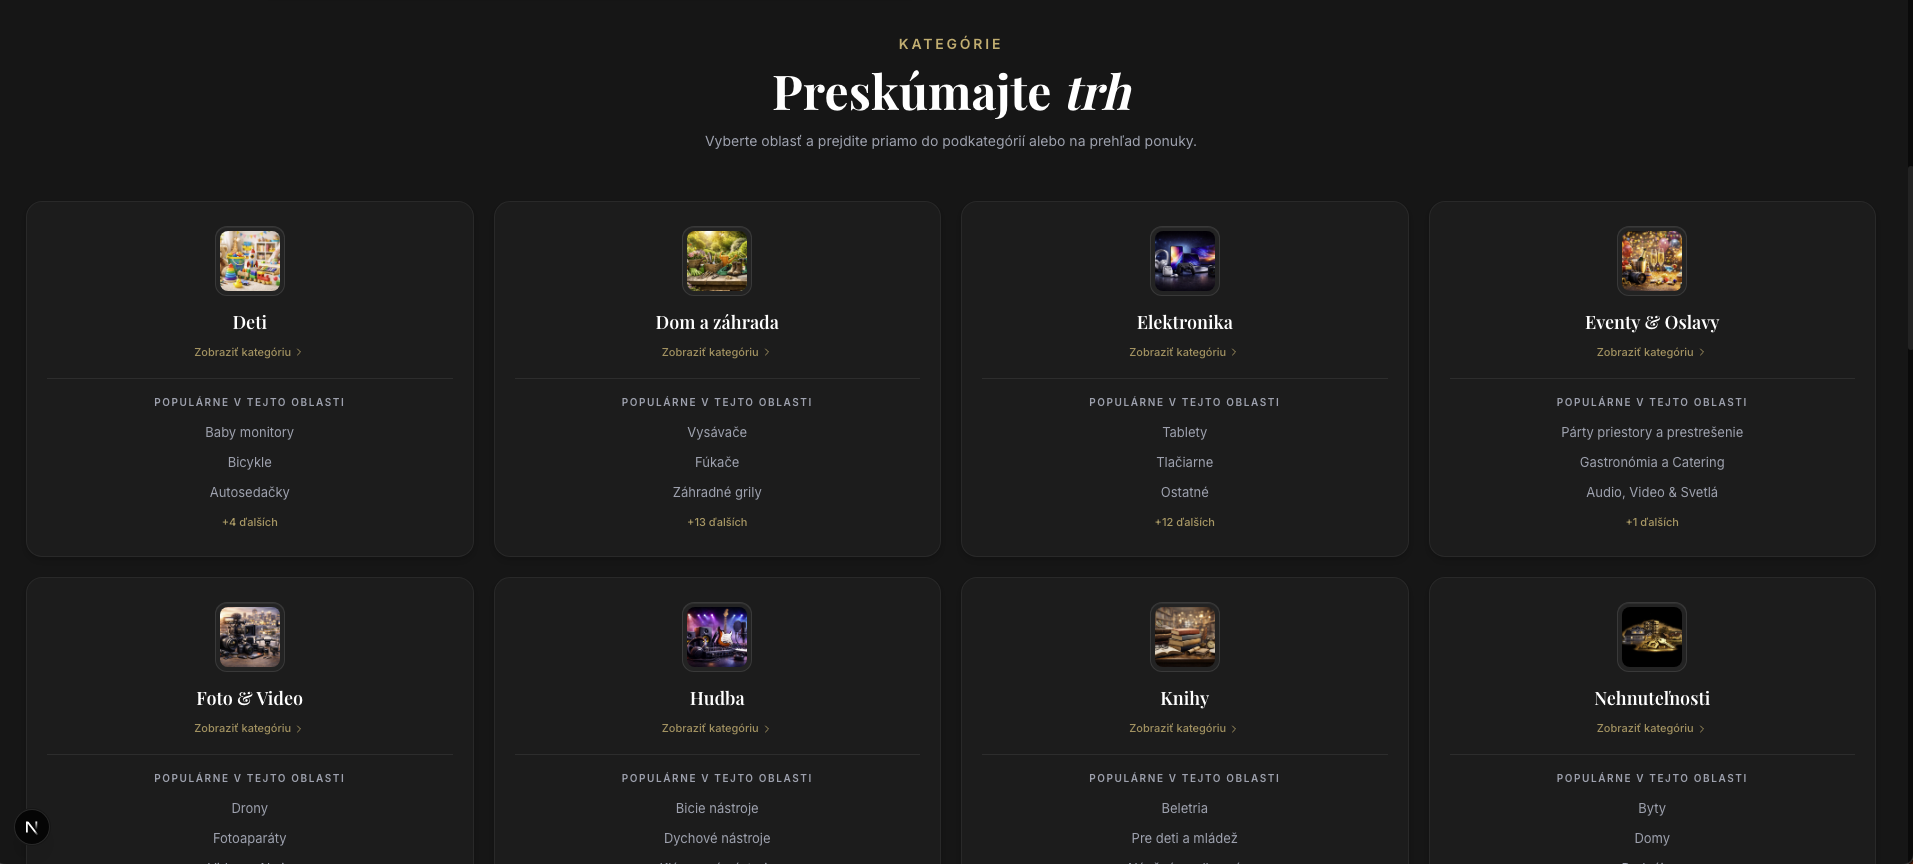
\includegraphics[width=\textwidth]{images/platforma_2.png}
\caption{Verejná platforma -- prehľad aktívnych inzerátov so zoznamovým zobrazením a postrannými filtrami}
\label{fig:platforma-2}
\end{figure}

\begin{figure}[htbp]
\centering
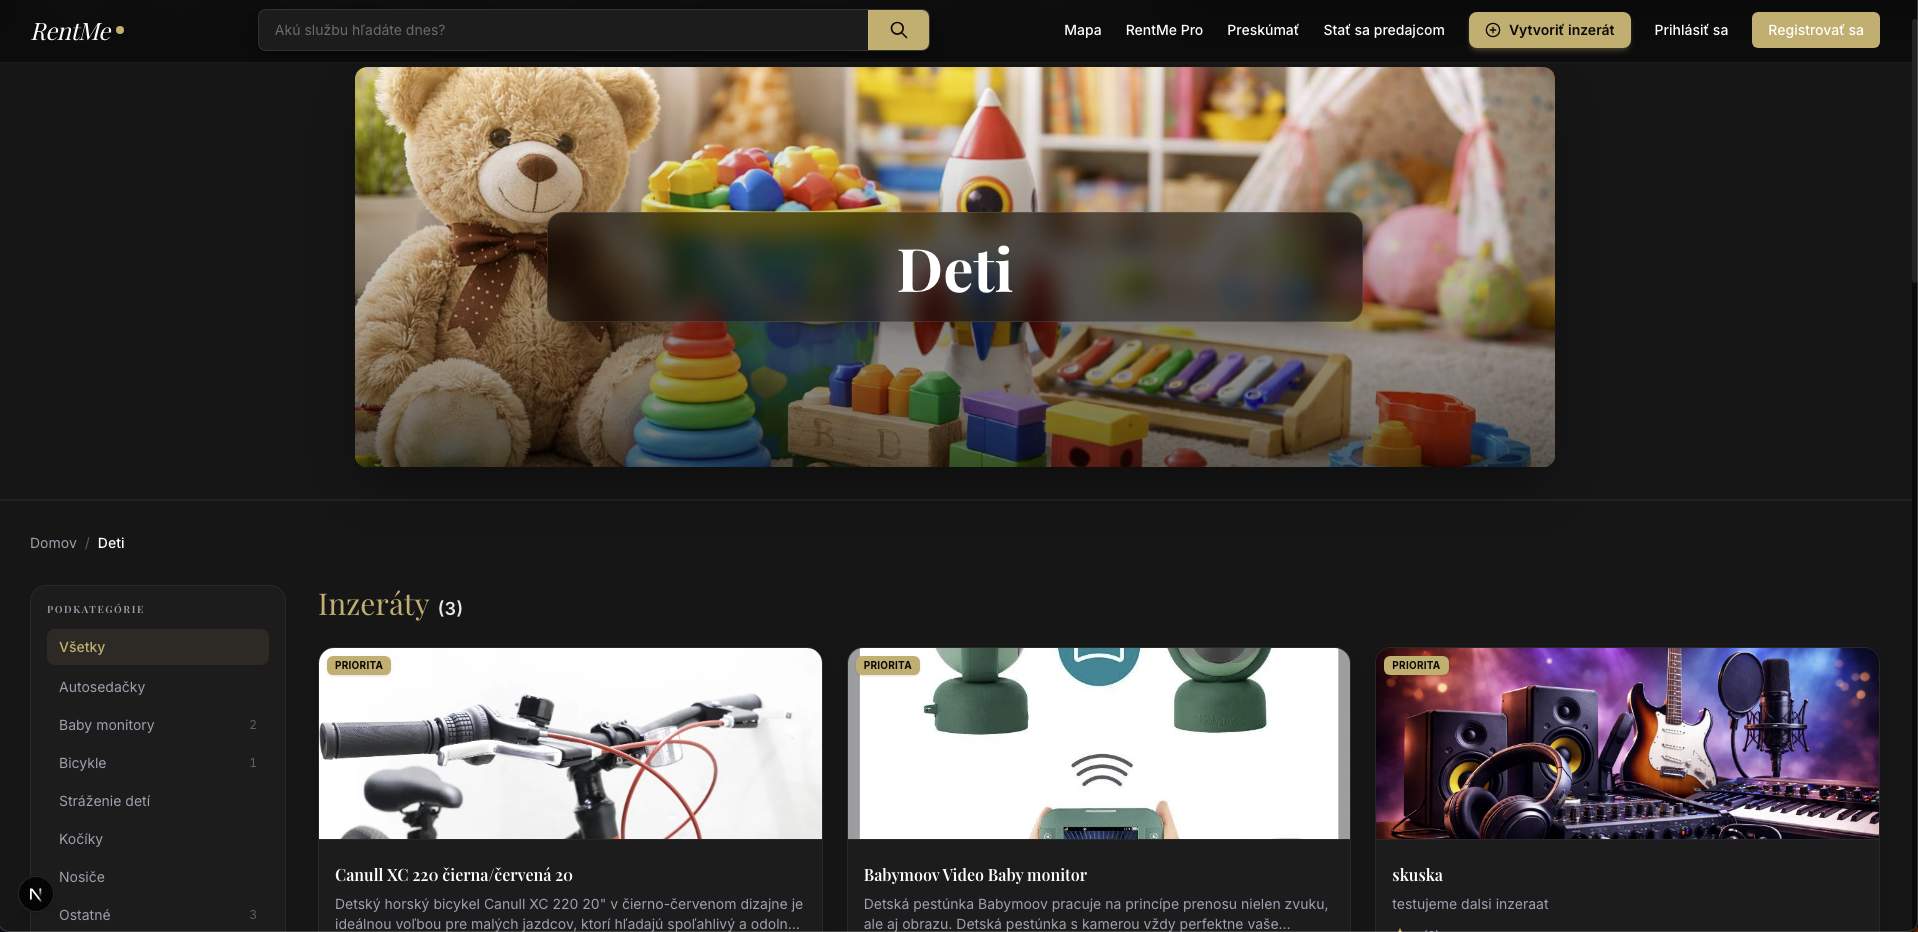
\includegraphics[width=\textwidth]{images/category_1.png}
\caption{Detail kategórie -- zoznam inzerátov v rámci zvolenej kategórie s hierarchickou navigáciou a SEO-optimalizovanou URL}
\label{fig:category-1}
\end{figure}

\begin{figure}[htbp]
\centering
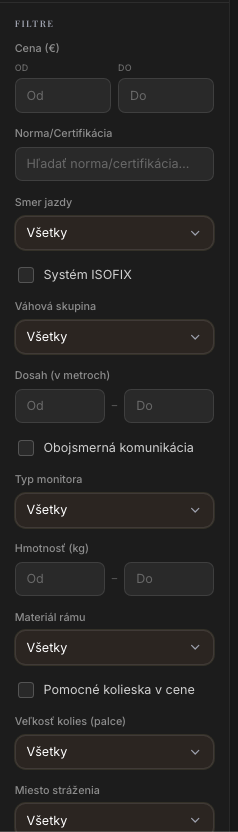
\includegraphics[width=0.7\textwidth]{images/filters.png}
\caption{Panel dynamických filtrov -- vstupy generované podľa konfigurácie kategórie (typy \texttt{TEXT}, \texttt{NUMBER}, \texttt{SELECT}, \texttt{MULTISELECT}, \texttt{BOOLEAN}, \texttt{DATE}, \texttt{RANGE})}
\label{fig:filters}
\end{figure}

\textbf{Mapové zobrazenie (Leaflet):} Stránka s mapou zobrazuje všetky aktívne inzeráty ako interaktívne markery (obr.~\ref{fig:platforma-3}). Dáta o polohe (latitúda, longitúda) sú načítané z endpointu \hlcode{GET /advertisements/map}. Keďže knižnica Leaflet pristupuje k objektu \hlcode{window}, ktorý na serveri neexistuje, komponent mapy je načítaný asynchrónne pomocou \hlcode{next/dynamic} s parametrom \hlcode{ssr: false}, čím sa predíde hydratačným chybám.

\begin{figure}[htbp]
\centering
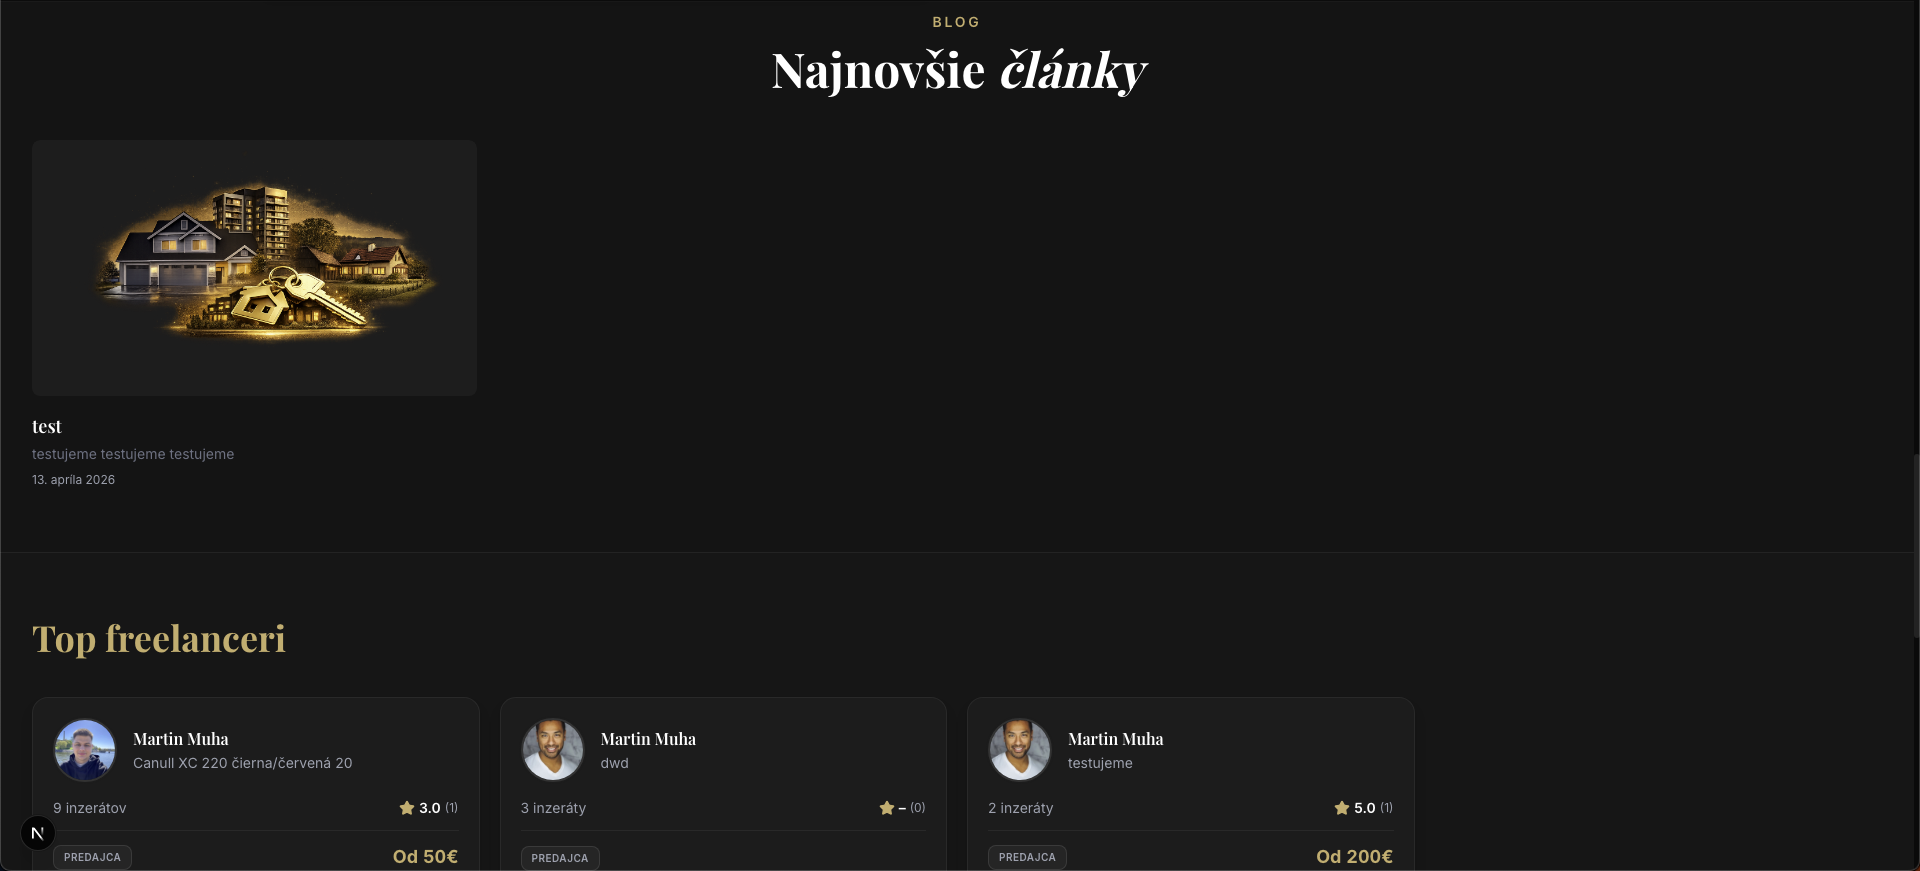
\includegraphics[width=\textwidth]{images/platforma_3.png}
\caption{Verejná platforma -- interaktívne mapové zobrazenie inzerátov implementované knižnicou Leaflet}
\label{fig:platforma-3}
\end{figure}

\textbf{Blog a statické stránky:} Obsah blogu a informačných stránok je spravovaný cez administračný panel a uložený v databáze ako HTML. Platforma ho zobrazuje vo forme staticky renderovaných stránok, ktoré sú automaticky generované pri každom requeste (SSR) alebo môžu byť cachovane (ISR), čo minimalizuje záťaž na databázu. Výslednú vizuálnu podobu sekcie blogu a informačných stránok dokumentuje obrázok~\ref{fig:platforma-4}.

\begin{figure}[htbp]
\centering
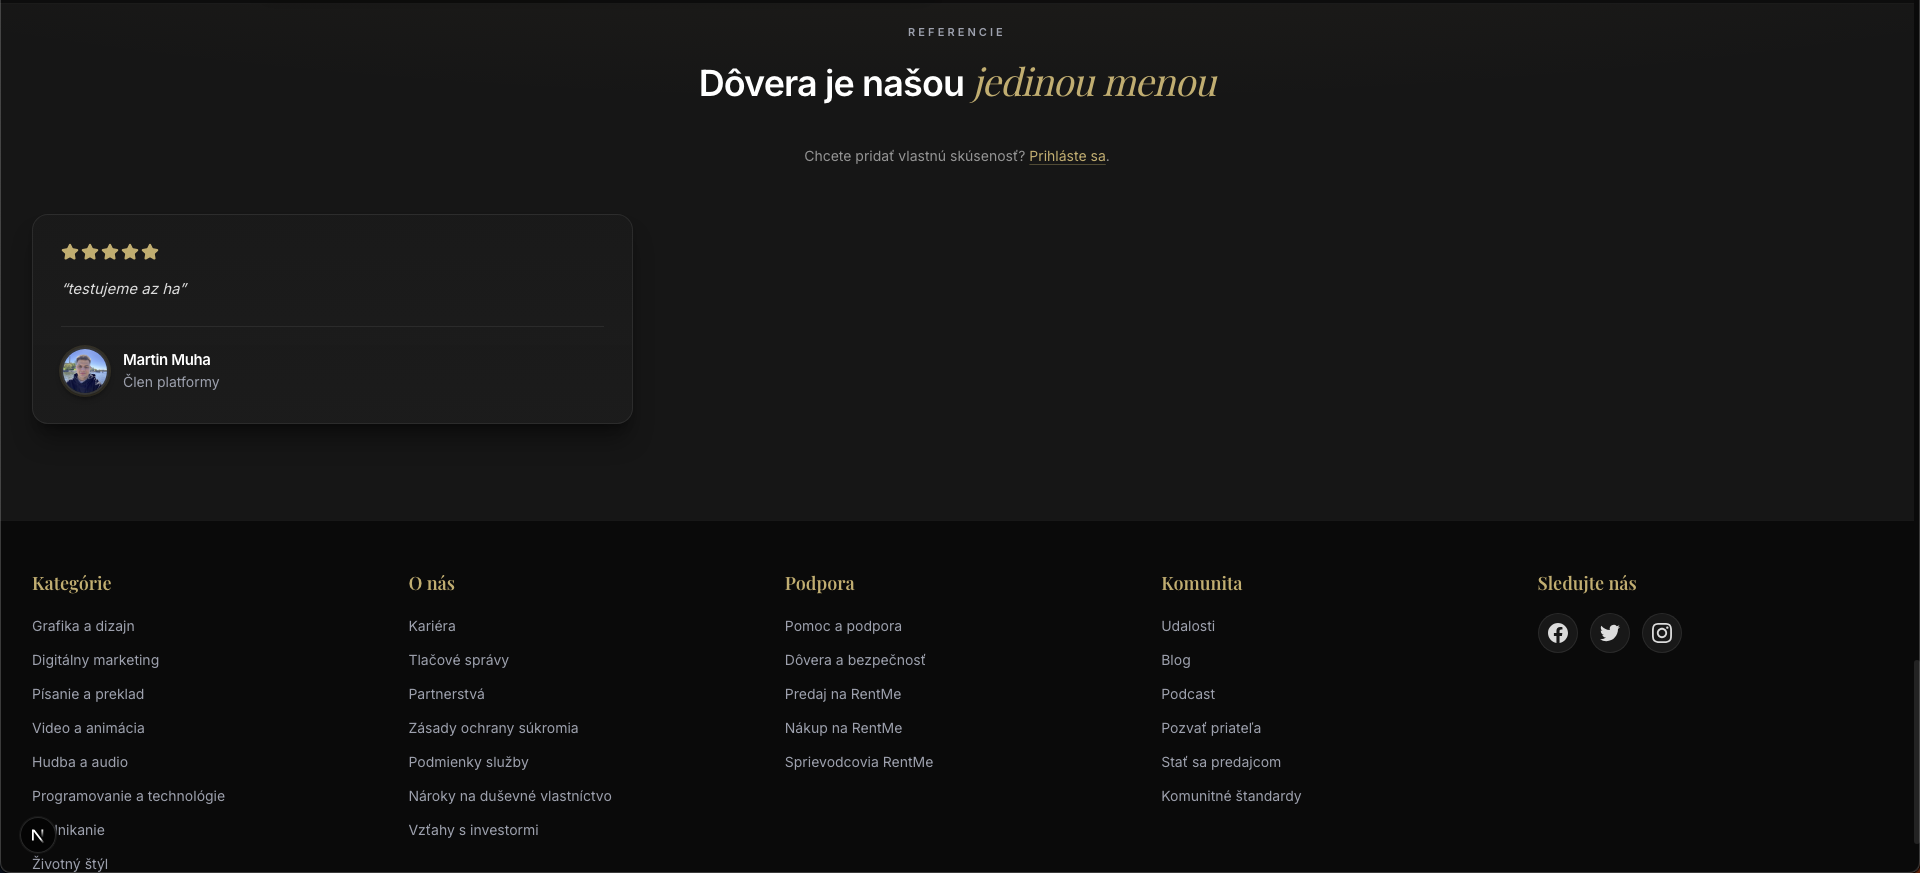
\includegraphics[width=\textwidth]{images/platforma_4.png}
\caption{Verejná platforma -- sekcia blogu a informačných stránok generovaných cez SSR z databázy}
\label{fig:platforma-4}
\end{figure}

\subsubsection{Používateľská zóna (správa inzerátov a profilu)}
\noindent
Aplikácia \hlcode{apps/user} je dostupná výhradne pre prihlásených používateľov. Autentifikácia je riešená prostredníctvom JWT tokenu, ktorý je po prihlásení uložený v HTTP-only cookie, čím je chránený pred útokmi XSS \parencite{hoffman2020websec}.

\textbf{Sprievodca tvorbou inzerátu (Wizard):} Namiesto jednoduchého formulára som implementoval viacstupňového sprievodcu (\emph{wizard}), ktorý vedie používateľa krok za krokom: výber kategórie~→ zadanie detailov a špecifikácií~→ nahratie fotografií~→ zadanie polohy na mape~→ odoslanie na schválenie. Tento prístup výrazne znižuje kognitívnu záťaž pri tvorbe inzerátu a prispieva k vyššej kvalite zadaných dát.

V prvom kroku sprievodcu (obr.~\ref{fig:inzerat-1}) si používateľ zvolí typ ponuky (služba alebo prenájom) a hierarchicky vyberie cieľovú kategóriu. Voľba kategórie následne určuje, aké dynamické filtre a špecifikácie sa zobrazia v druhom kroku.

\begin{figure}[htbp]
\centering
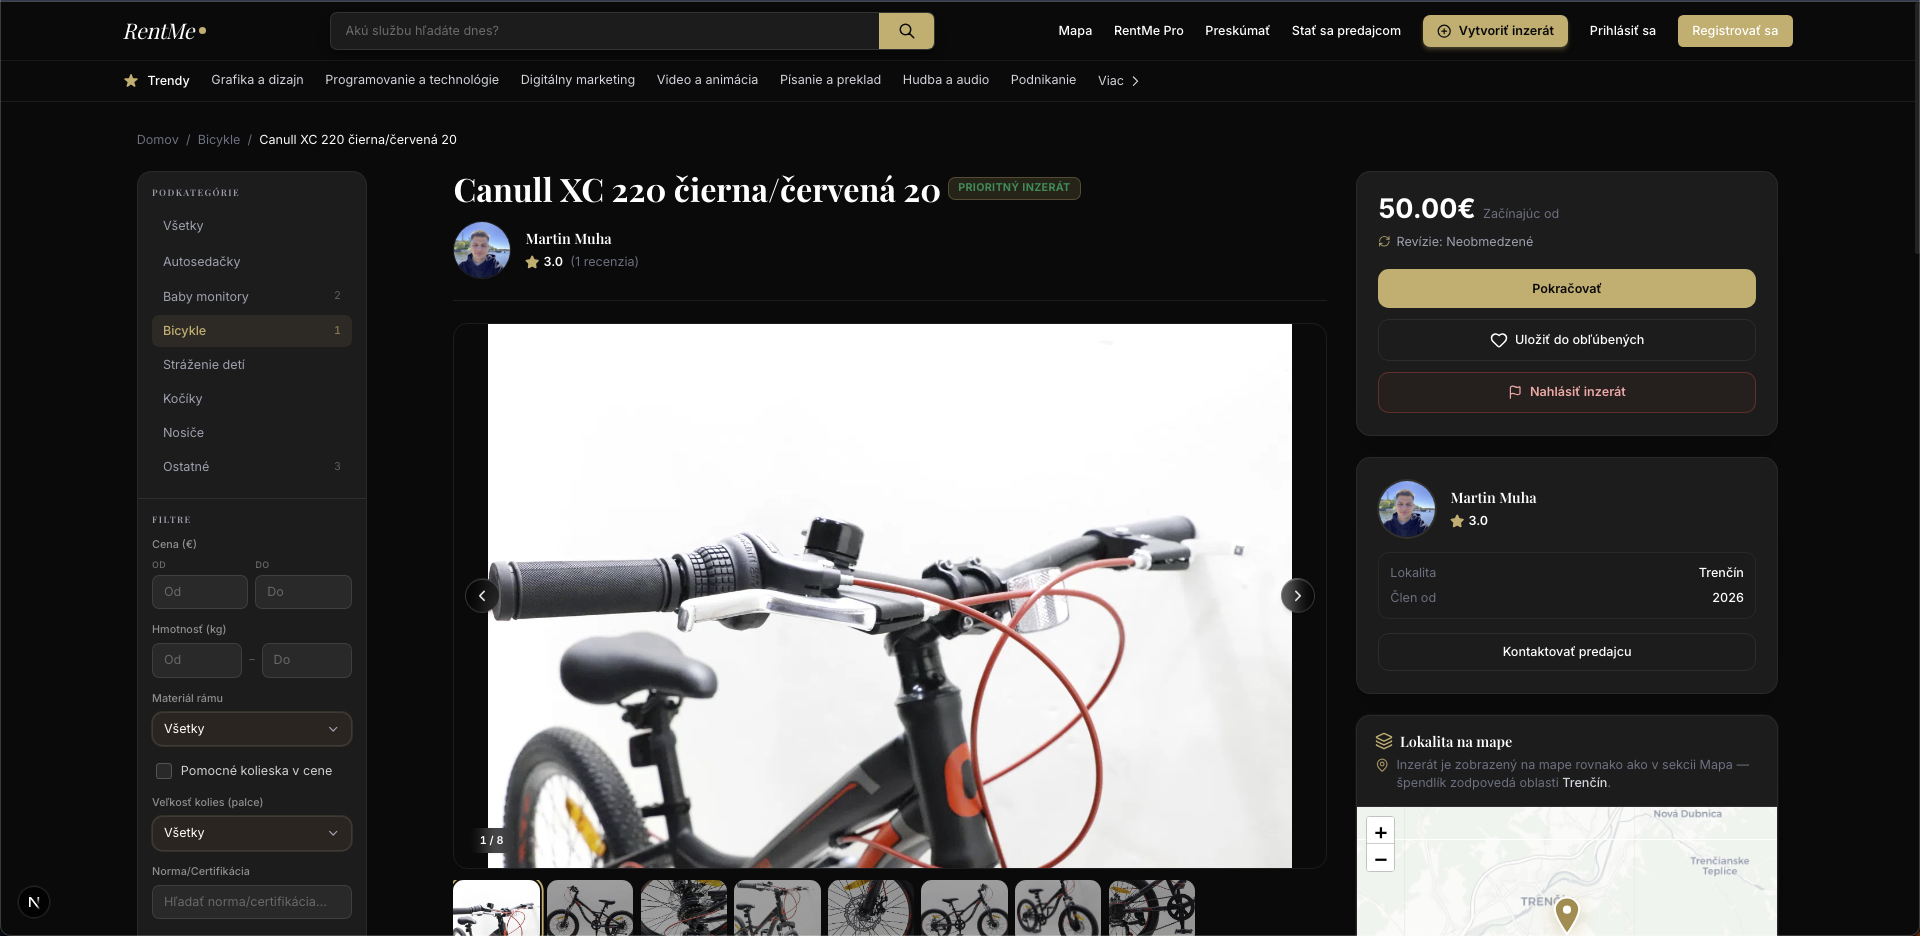
\includegraphics[width=\textwidth]{images/inzerat_1.png}
\caption{Sprievodca tvorbou inzerátu -- krok~1: výber typu ponuky (služba alebo prenájom) a hierarchický výber kategórie}
\label{fig:inzerat-1}
\end{figure}

V druhom kroku používateľ vyplní základné údaje o inzeráte -- názov, popis, cenu a hodnoty dynamických špecifikácií, ktoré sú generované podľa konfigurácie zvolenej kategórie (obr.~\ref{fig:inzerat-2}). Tieto údaje sú serializované do JSON štruktúry \hlcode{specifications} a uložené v databáze.

\begin{figure}[htbp]
\centering
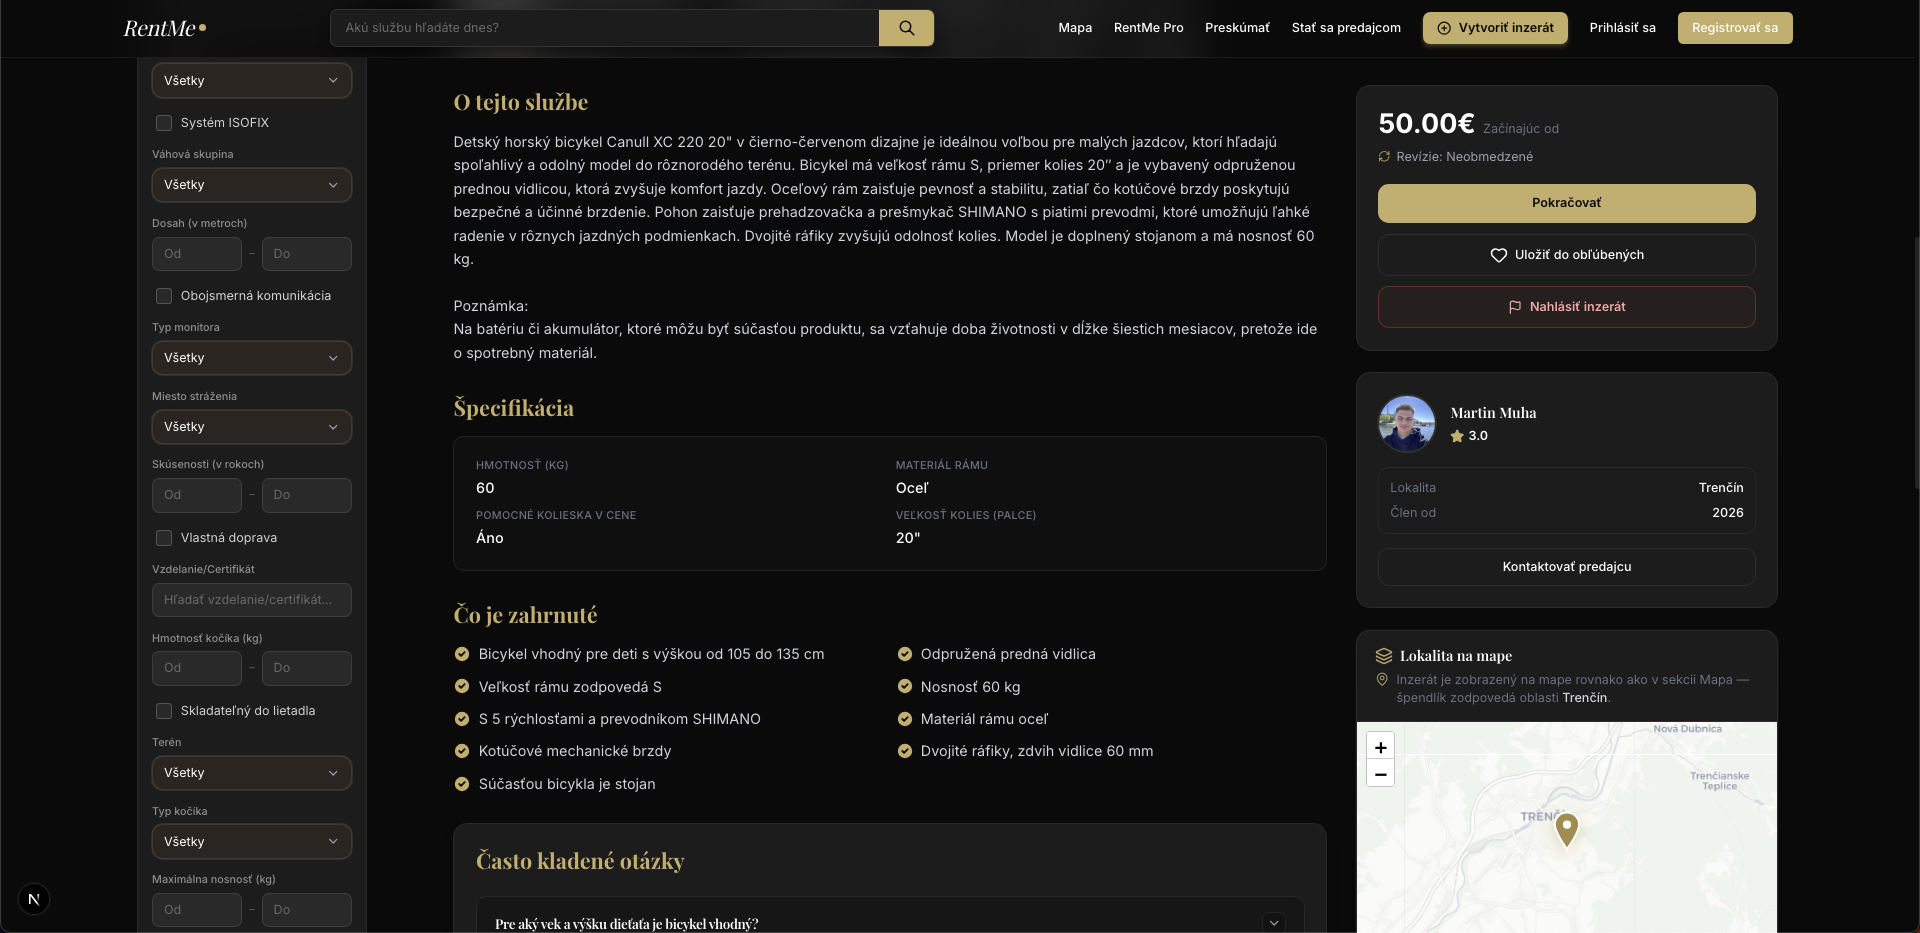
\includegraphics[width=\textwidth]{images/inzerat_2.png}
\caption{Sprievodca tvorbou inzerátu -- krok~2: zadanie základných údajov (názov, popis, cena) a dynamických špecifikácií podľa zvolenej kategórie}
\label{fig:inzerat-2}
\end{figure}

Tretí krok je venovaný obrazovej dokumentácii ponuky a definícii balíčkov služieb (obr.~\ref{fig:inzerat-3}). Pre kategórie typu \hlcode{SERVICE} môže používateľ definovať viacero variantov balíčkov s rozdielnym rozsahom a cenou, čo je inšpirované modelom platformy Fiverr.

\begin{figure}[htbp]
\centering
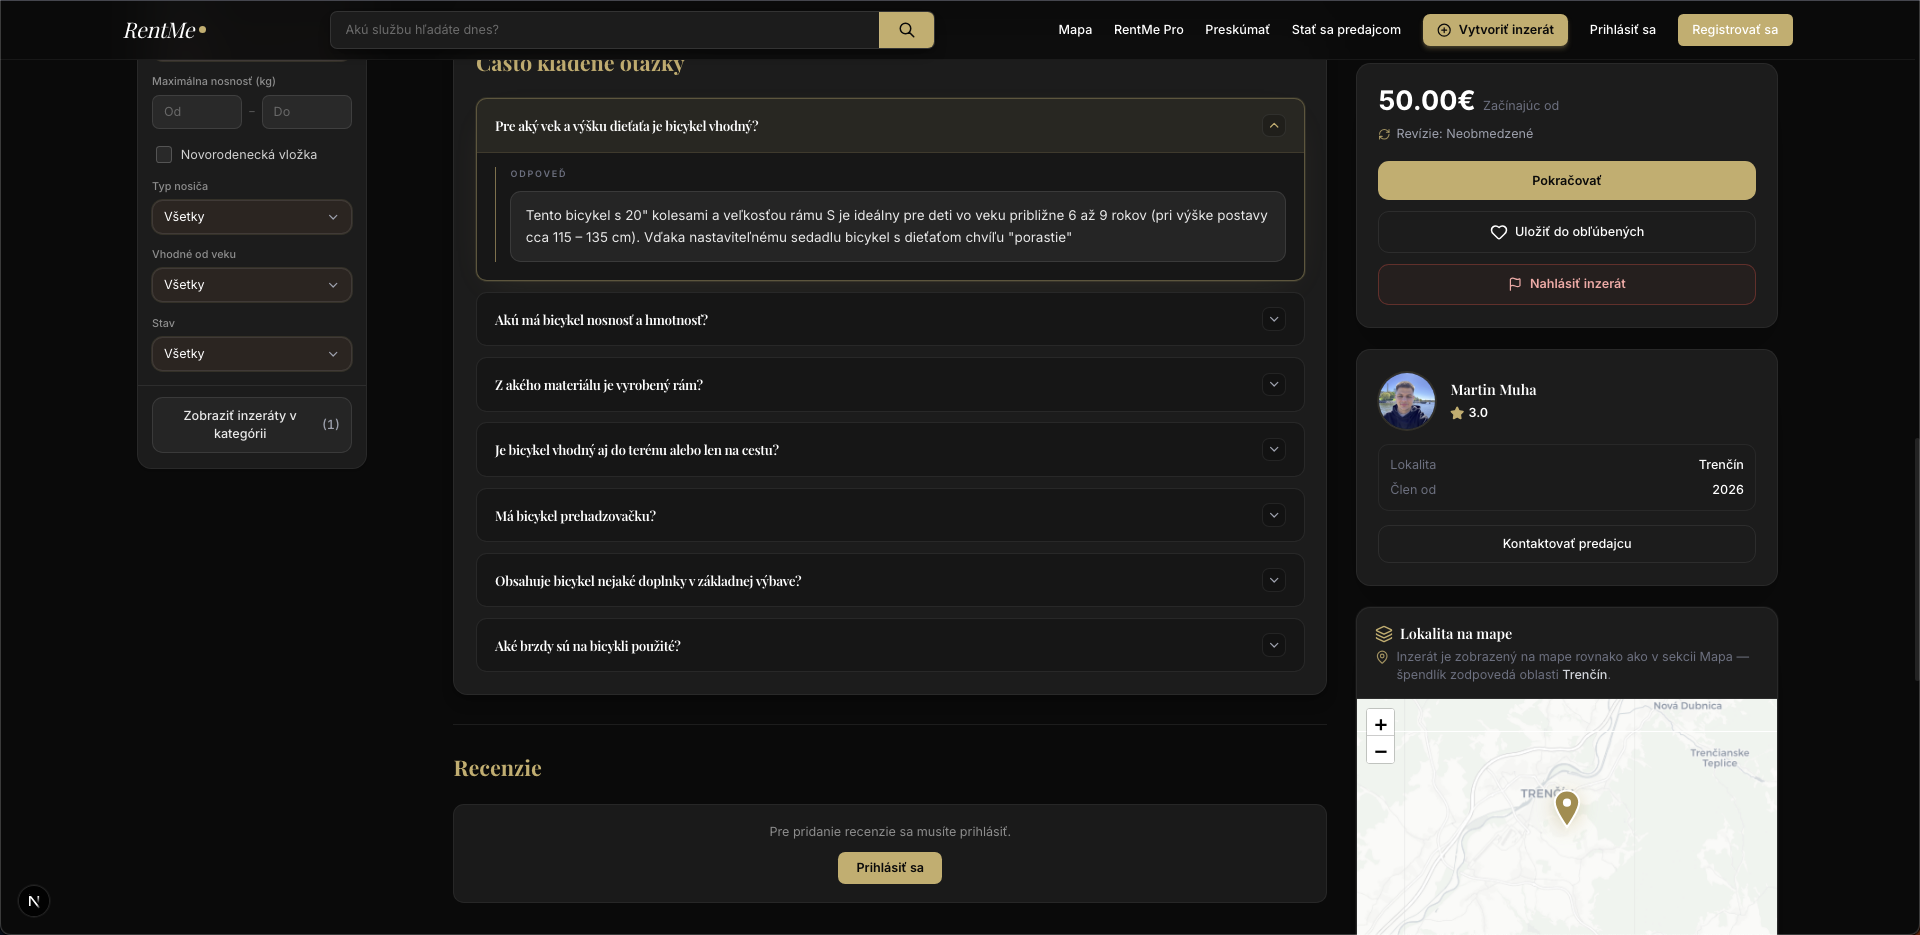
\includegraphics[width=\textwidth]{images/inzerat_3.png}
\caption{Sprievodca tvorbou inzerátu -- krok~3: nahrávanie obrazovej dokumentácie a definícia balíčkov služieb}
\label{fig:inzerat-3}
\end{figure}

Posledný krok sprievodcu zhromažďuje geografické údaje cez interaktívnu mapu Leaflet a umožňuje finálne odoslanie inzerátu na schválenie do moderačnej fronty (obr.~\ref{fig:inzerat-4}). Po odoslaní získa inzerát stav \hlcode{PENDING} a čaká na schválenie administrátorom.

\begin{figure}[htbp]
\centering
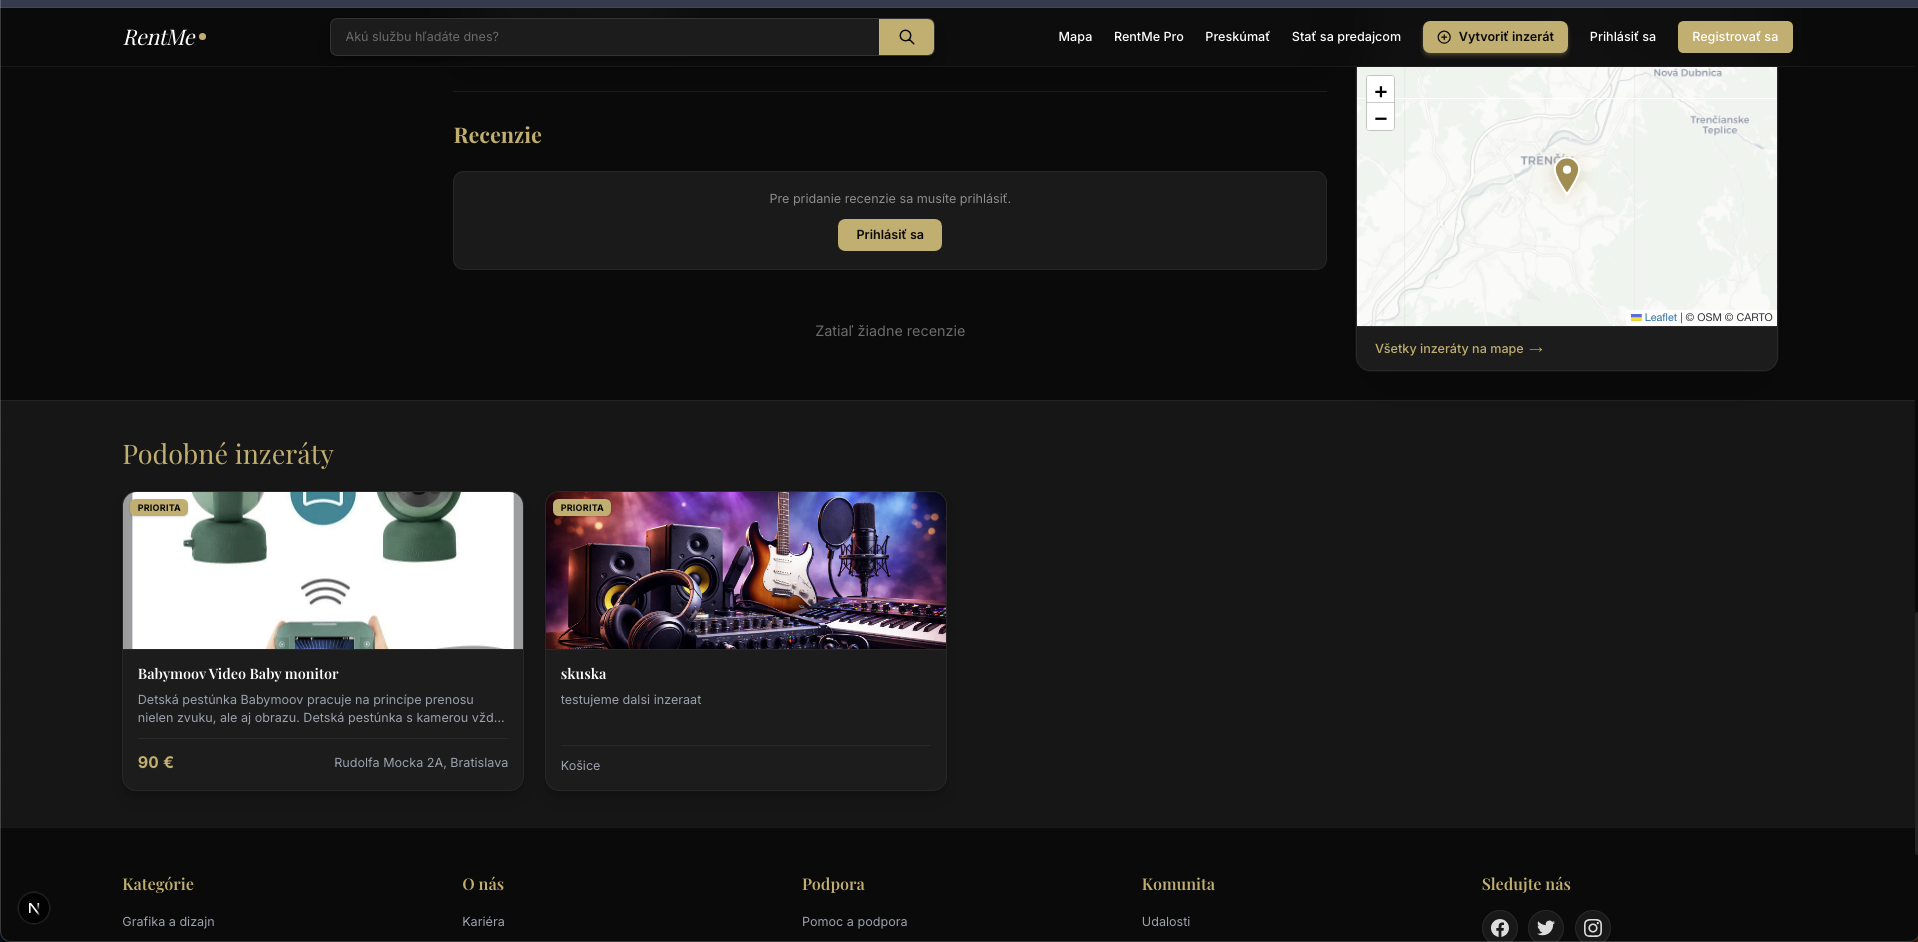
\includegraphics[width=\textwidth]{images/inzerat_4.png}
\caption{Sprievodca tvorbou inzerátu -- krok~4: výber polohy na interaktívnej mape (Leaflet) a finálne odoslanie inzerátu na schválenie}
\label{fig:inzerat-4}
\end{figure}

\textbf{Správa inzerátov:} Dashboard používateľa zobrazuje všetky jeho inzeráty vrátane ich aktuálneho stavu (\hlcode{PENDING}~--~čakajúci na schválenie, \hlcode{DRAFT}~--~rozpracovaný koncept, \hlcode{ACTIVE}~--~viditeľný, \hlcode{INACTIVE}~--~deaktivovaný používateľom, \hlcode{ARCHIVED}~--~archivovaný) a štatistík zobrazení. Používateľ môže inzeráty editovať, deaktivovať alebo zmazať. Prehľadovú stránku profilu predajcu so zoznamom jeho aktívnych inzerátov dokumentuje obrázok~\ref{fig:profile-inzerat}.

\begin{figure}[htbp]
\centering

\includegraphics[width=\textwidth]{images/profile-inzerat.png}
\caption{Verejný profil predajcu -- prehľad aktívnych inzerátov, kontaktné údaje a hodnotenia získané od ostatných používateľov platformy}
\label{fig:profile-inzerat}
\end{figure}

Okrem viacstupňového sprievodcu poskytuje aplikácia aj klasický jednostranový formulár (obr.~\ref{fig:pridat-inzerat} a~\ref{fig:pridat-inzerat-1}) určený pre používateľov, ktorí preferujú rýchlejšie vytvorenie inzerátu bez vedeného procesu. Formulár zhromažďuje rovnaký rozsah údajov (kategória, špecifikácie, fotografie, lokalita) ako wizard, ale prezentuje ich naraz s validáciou na strane klienta.

\begin{figure}[htbp]
\centering
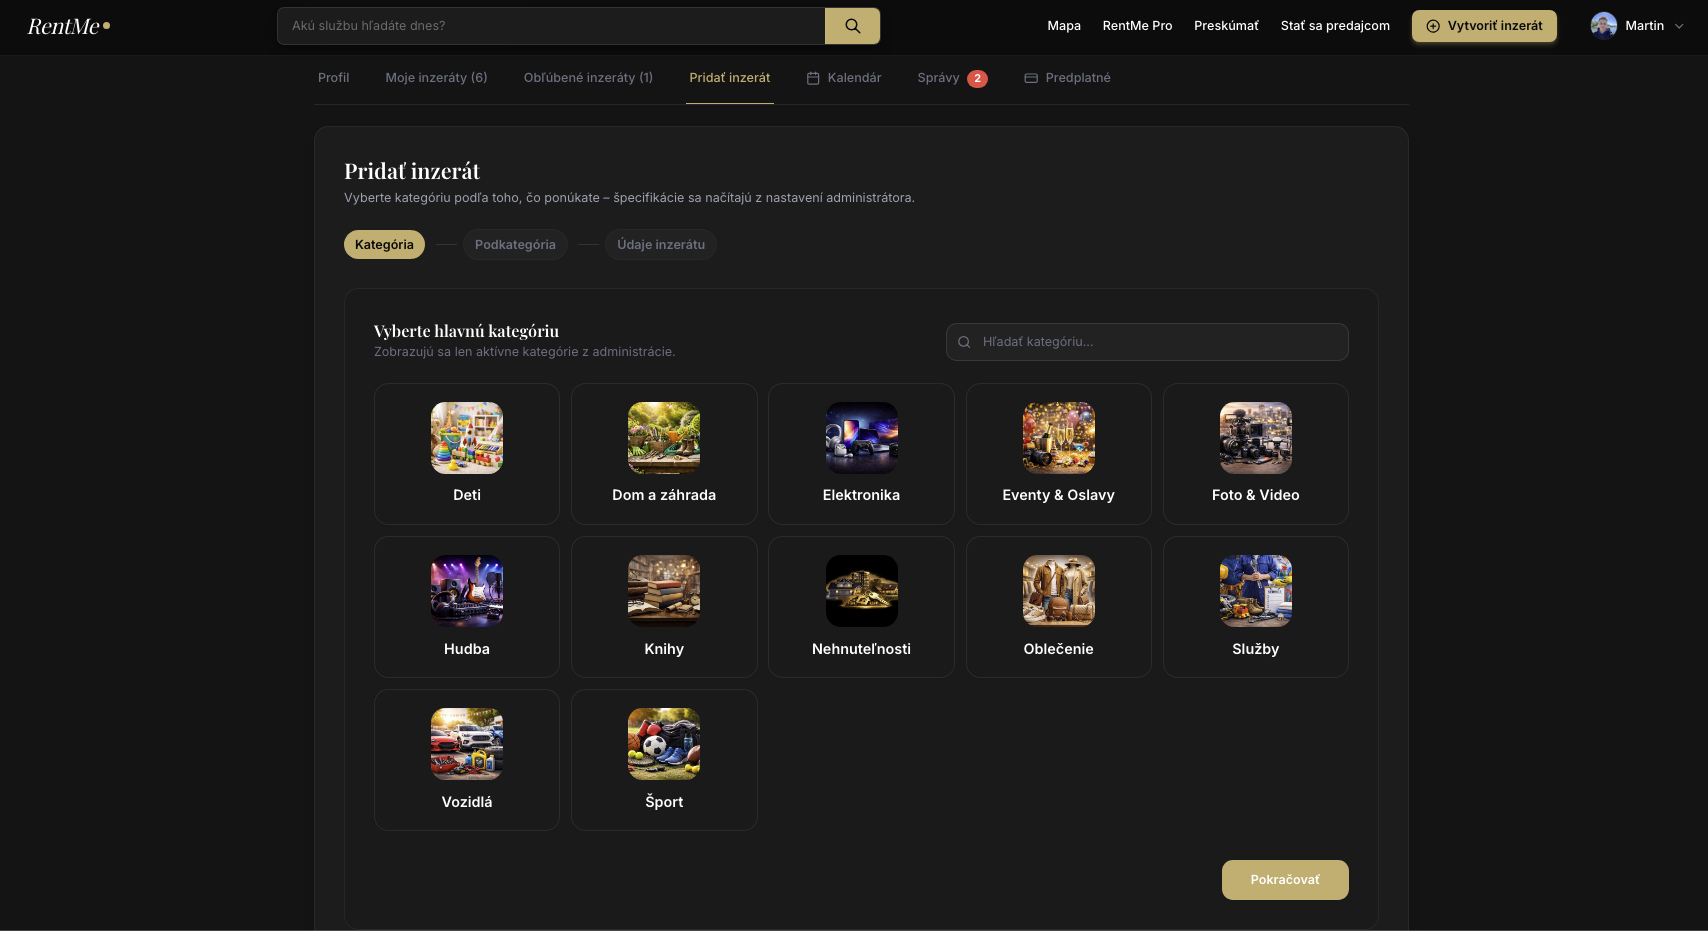
\includegraphics[width=\textwidth]{images/pridat-inzerat.png}
\caption{Pridanie inzerátu -- horná časť formulára so základnými údajmi (typ ponuky, kategória, názov, popis, cena) a možnosťou nahratia fotografií}
\label{fig:pridat-inzerat}
\end{figure}

\begin{figure}[htbp]
\centering
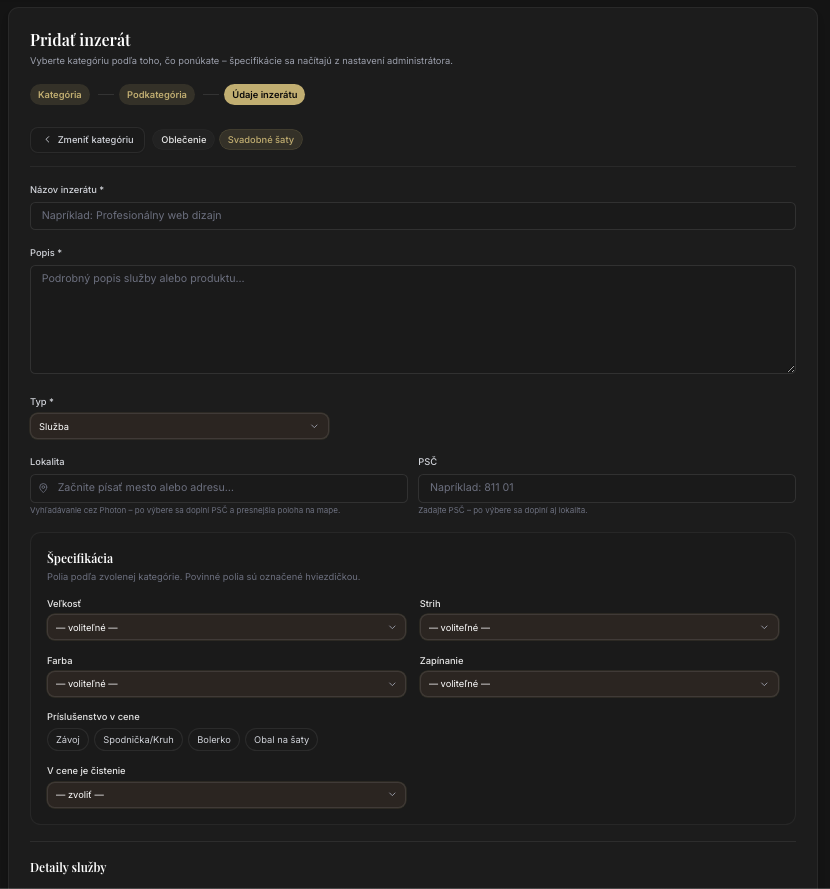
\includegraphics[width=\textwidth]{images/pridat-inzerat_1.png}
\caption{Pridanie inzerátu -- spodná časť formulára s dynamickými špecifikáciami, výberom polohy na mape Leaflet a tlačidlom na odoslanie do moderačnej fronty}
\label{fig:pridat-inzerat-1}
\end{figure}

\textbf{Komunikácia -- Inbox:} Modul správ zobrazuje zoznam konverzácií (dopytov k inzerátom) a umožňuje odpovedanie v reálnom čase. Systémové notifikácie (napr. o schválení inzerátu) sú vizuálne odlíšené od bežných správ od iných používateľov.

\textbf{Obľúbené položky:} Stránka zobrazuje inzeráty uložené používateľom do obľúbených. Pridávanie a odoberanie z obľúbených je realizované optimistickým UI updatem -- tlačidlo reaguje okamžite bez čakania na odpoveď servera, čo zvyšuje vnímaný výkon.

\textbf{Predajné balíky a platby:} Aplikácia podporuje štyri úrovne predajného plánu (\hlcode{SellerPlan}) -- \hlcode{STANDARD} (zdarma), \hlcode{PLUS} (8,99\,€/mesiac), \hlcode{PRO} (16,99\,€/mesiac) a \hlcode{FIRMA} (39\,€/mesiac) -- ktoré sa líšia počtom prioritných inzerátov, mierou zvýraznenia vo vyhľadávaní a rozsahom analytických funkcií. Výber balíka je dostupný priamo v používateľskej zóne (obr.~\ref{fig:platba-1}). Detail jednotlivej platby so sumou, obdobím a referenciou na inzerát, vrátane stavu definovaného enumerátorom \hlcode{PaymentStatus} (\hlcode{PENDING}, \hlcode{COMPLETED}, \hlcode{FAILED}, \hlcode{CANCELLED}, \hlcode{REFUNDED}), je dokumentovaný na obrázku~\ref{fig:platby-2}.

\begin{figure}[htbp]
\centering
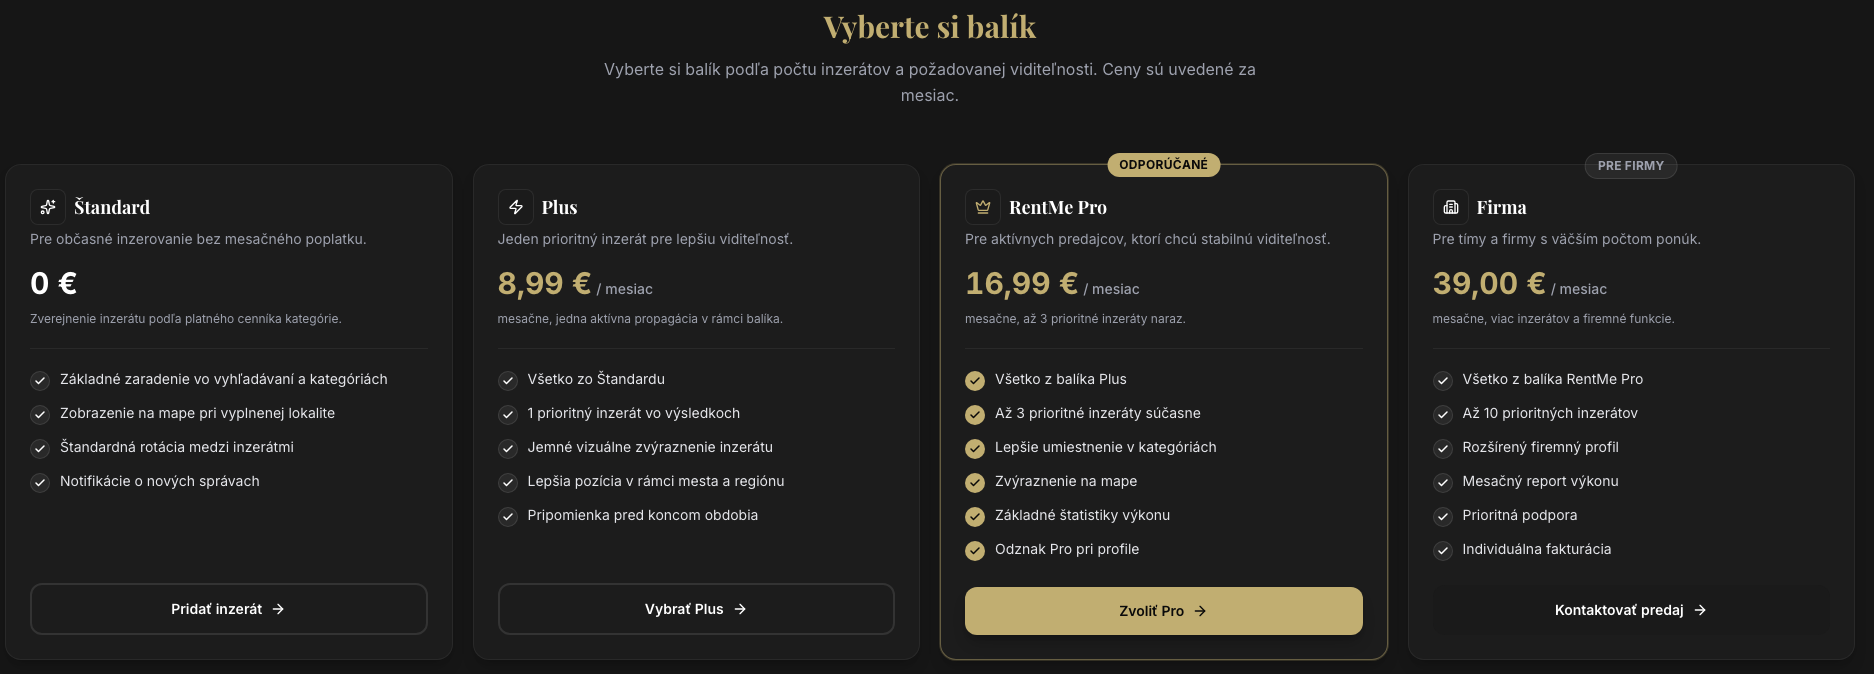
\includegraphics[width=\textwidth]{images/platba-1.png}
\caption{Výber predajného balíka -- štyri úrovne \texttt{SellerPlan} (Štandard~--~0\,€/mesiac, Plus~--~8,99\,€/mesiac, RentMe Pro~--~16,99\,€/mesiac, Firma~--~39\,€/mesiac) s porovnaním funkcií a viditeľnosti inzerátov}
\label{fig:platba-1}
\end{figure}

\begin{figure}[htbp]
\centering
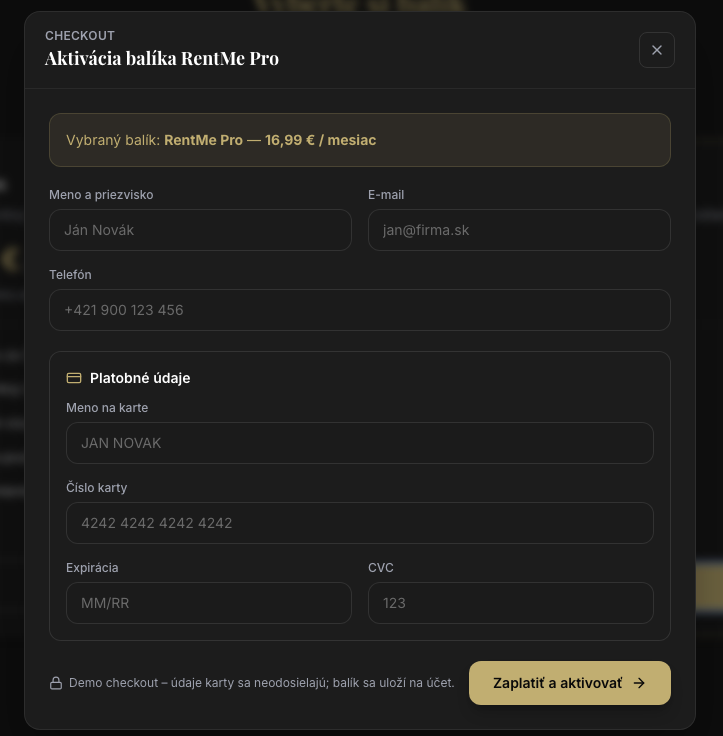
\includegraphics[width=\textwidth]{images/platby-2.png}
\caption{Modul platieb -- detail jednotlivej transakcie so sumou, obdobím prenájmu, referenciou na inzerát a časovou osou zmien stavu}
\label{fig:platby-2}
\end{figure}

\subsubsection{Administračný panel (CMS, vizuálny editor GrapesJS, štatistiky)}
\noindent
Aplikácia \hlcode{apps/admin} poskytuje správcom platformy kompletné nástroje na správu obsahu, používateľov a konfigurácie systému. Je chránená dvojvrstvovým overovaním: platným JWT tokenom a rolou \hlcode{ADMIN}, pričom prístup začína na dedikovanej prihlasovacej obrazovke s vlastným brandingom (obr.~\ref{fig:admin-login}).

\begin{figure}[htbp]
\centering
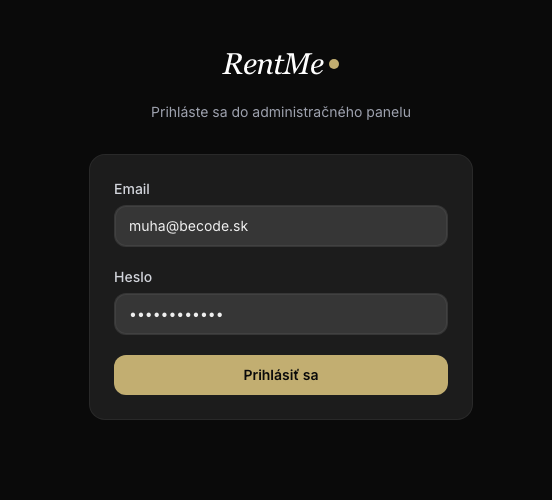
\includegraphics[width=0.78\textwidth]{images/admin-login.png}
\caption{Prihlasovacia obrazovka administračného panela RentMe -- minimalistický dizajn s tmavou paletou a prémiovým zlatým akcentom}
\label{fig:admin-login}
\end{figure}

Po úspešnej autentifikácii je administrátor presmerovaný na hlavnú nástenku (\emph{dashboard}), ktorá agreguje kľúčové metriky platformy (celkový počet používateľov, aktívnych používateľov, inzerátov a aktívnych inzerátov) a sprístupňuje rýchle akcie pre najčastejšie pracovné toky -- nový inzerát, nová kategória, moderácia obsahu, nastavenia (obr.~\ref{fig:admin-dashboard}).

\begin{figure}[htbp]
\centering
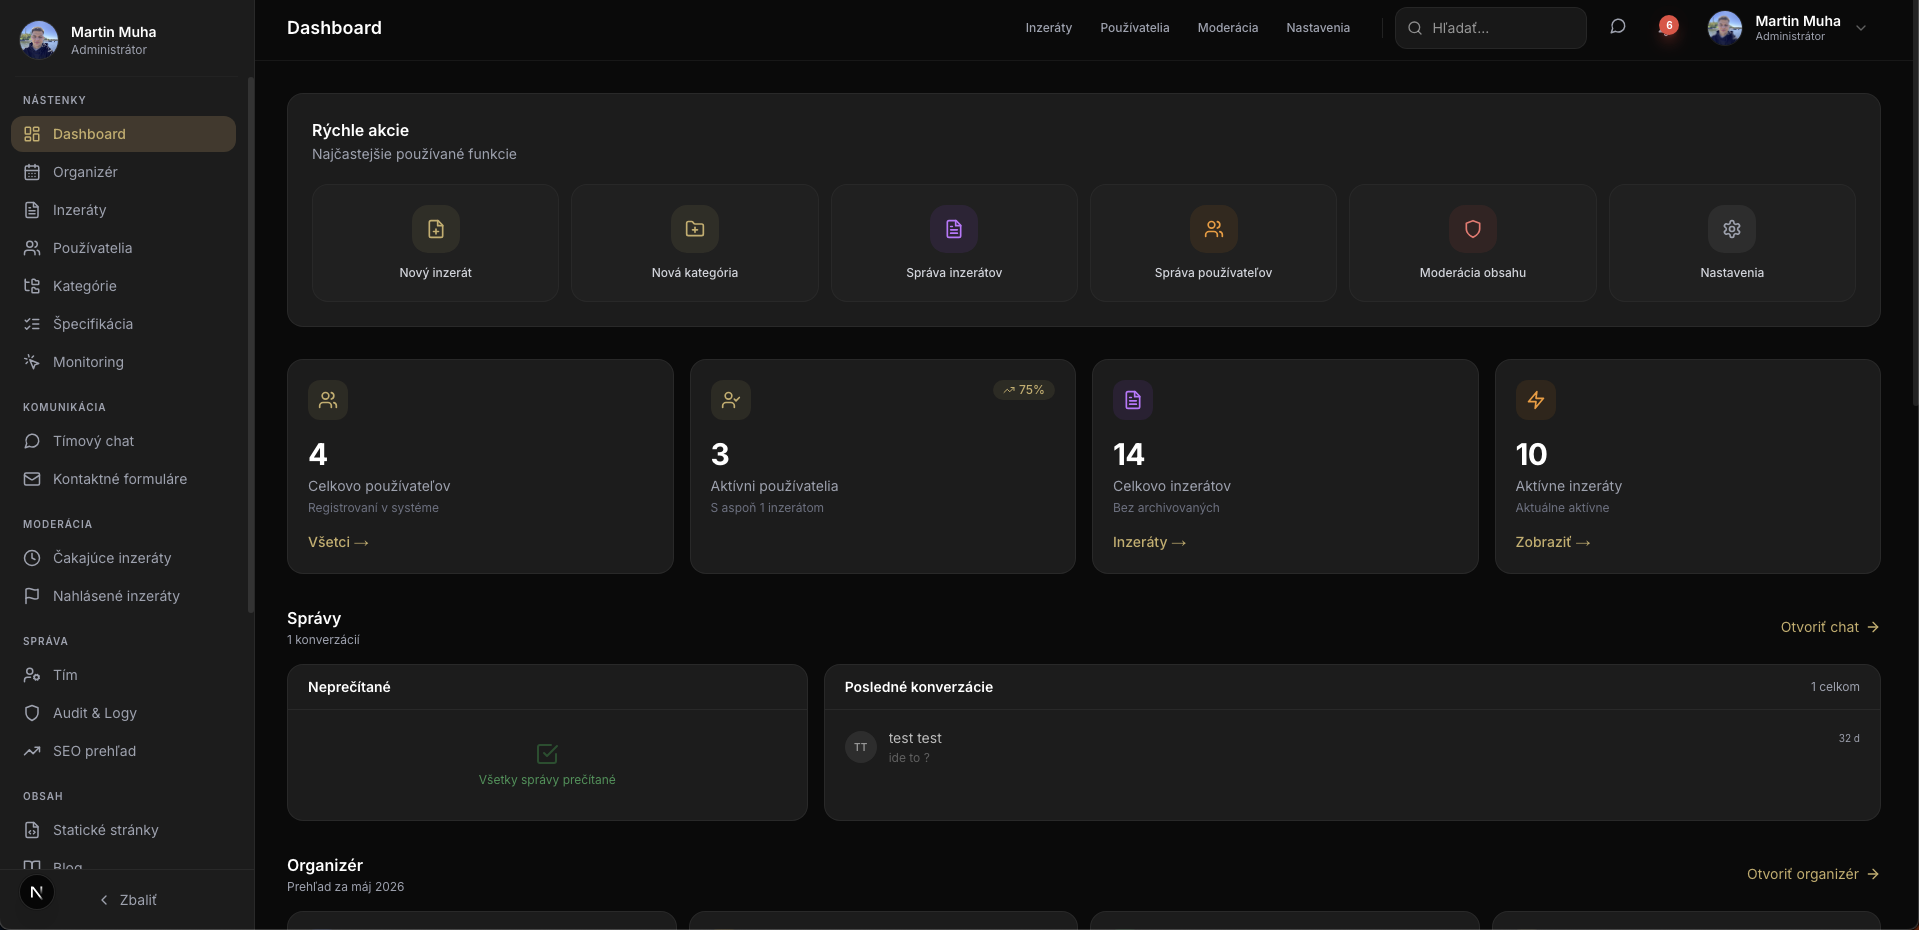
\includegraphics[width=\textwidth]{images/admin.png}
\caption{Hlavná nástenka admin panela -- bočná navigácia (Nástenky, Komunikácia, Moderácia, Správa, Obsah), rýchle akcie, agregované metriky a panel s nedávnymi konverzáciami}
\label{fig:admin-dashboard}
\end{figure}

\textbf{Moderácia inzerátov:} Hlavnou obrazovkou admina je zoznam inzerátov čakajúcich na schválenie (\hlcode{PENDING}). Pre každý inzerát zobrazuje náhľad, fotografie a lokalizáciu na mape. Administrátor môže inzerát schváliť (zmena stavu na \hlcode{ACTIVE}), zamietnuť alebo archivovať. Každá akcia automaticky odošle systémovú správu inzerentovi.

\textbf{Vizuálny editor GrapesJS:} Na správu statických stránok a blogových príspevkov som integroval open-source editor GrapesJS. Umožňuje administrátorovi vytvárať a upravovať HTML obsah stránok drag-and-drop spôsobom bez znalosti HTML kódu. Výsledný HTML kód je uložený do databázy a zobrazovaný na verejnej platforme. Aj tu bolo potrebné riešiť kompatibilitu s SSR pomocou asynchrónneho načítavania modulu cez \hlcode{next/dynamic} s voľbou \hlcode{ssr:\,false}, ktorá zaručuje inicializáciu editora výhradne v prehliadači.

\textbf{Správa kategórií a filtrov:} Admin panel umožňuje vytvárať a editovať hierarchiu kategórií (hlavné kategórie, podkategórie) a priraďovať im dynamické filtre. Každý filter má definovaný typ z enumerátora \hlcode{FilterType}~--~\hlcode{TEXT} (Text), \hlcode{NUMBER} (Číslo), \hlcode{SELECT} (Výber jednej možnosti), \hlcode{MULTISELECT} (Výber viacerých možností), \hlcode{BOOLEAN} (Áno/Nie), \hlcode{DATE} (Dátum) a \hlcode{RANGE} (Rozsah)~--~spolu s názvom, popisom a poradím zobrazenia. Zmeny sa okamžite premietnu do vyhľadávacieho panela na verejnej platforme bez nutnosti nasadenia novej verzie aplikácie.

\textbf{Analytický dashboard:} Panel štatistík zobrazuje grafy kliknutí na inzeráty v čase, rozdelenie záujmu podľa kategórií a segmentáciu podľa typu používateľa (obr.~\ref{fig:admin-stats}). Dáta pochádzajú z tabuľky \hlcode{ClickEvent}, ktorá je plnená asynchrónne pri každom zobrazení detailu inzerátu \parencite{winters2020swe}. Časové obdobie štatistík je prepínateľné medzi 7 dňami, 30 dňami a 3 mesiacmi, pričom interaktívny tooltip umožňuje sledovať presné hodnoty v konkrétnom dni.

\begin{figure}[htbp]
\centering
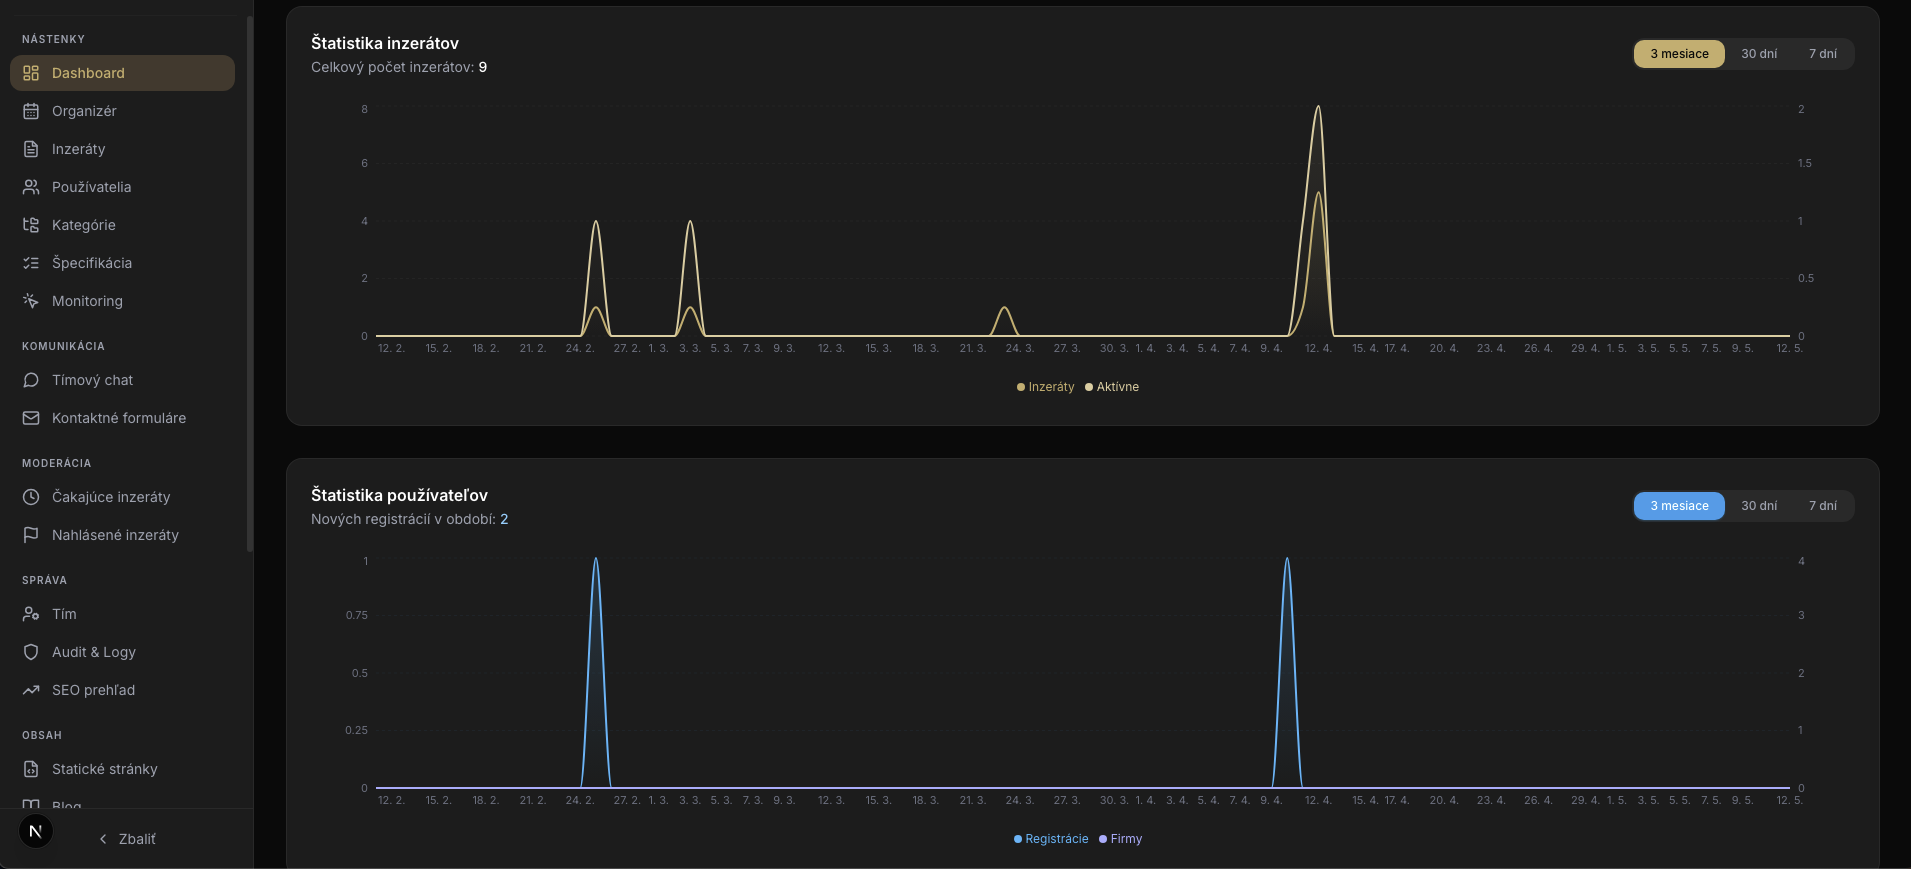
\includegraphics[width=\textwidth]{images/admin-stats.png}
\caption{Štatistická sekcia admin panela -- časové rady inzerátov (zlatá krivka) a registrácií používateľov (modrá krivka) s prepínateľným obdobím (7 dní / 30 dní / 3 mesiace) a interaktívnym tooltipom pre detailné hodnoty v konkrétnom dni}
\label{fig:admin-stats}
\end{figure}

\subsection{Bezpečnostné aspekty: Hashovanie hesiel (bcrypt), validácia vstupov (class-validator) a ochrana účtov (banovanie)}
\noindent
Bezpečnosť je prierezovou vlastnosťou celého systému. Navrhnuté opatrenia pokrývajú tri hlavné oblasti: ochranu hesiel, integritu vstupných dát a správu používateľských účtov \parencite{hoffman2020websec}.

\textbf{Hashovanie hesiel (bcrypt):} Heslá používateľov nie sú nikdy ukladané v čitateľnej podobe. Pred uložením sú transformované pomocou adaptívneho hašovacieho algoritmu bcrypt s hodnotou \hlcode{saltRounds = 10} \parencite{hoffman2020websec}. Bcrypt je úmyselne pomalý -- sťažuje útoky hrubou silou (\emph{brute-force}) a dúhové tabuľky (\emph{rainbow tables}). Pri prihlásení sa zadané heslo porovná s uloženým hašom pomocou funkcie \hlcode{bcrypt.compare()}, pričom pôvodné heslo nikdy neopúšťa pamäť servera.

\textbf{Validácia vstupov (class-validator):} Každá prichádzajúca HTTP požiadavka prechádza validáciou pomocou globálne nastaveného \hlcode{ValidationPipe} v konfigurácii NestJS \parencite{hoffman2020websec}. Pravidlá validácie sú deklarované pomocou dekorátorov z knižnice \hlcode{class-validator} priamo v DTO triedach -- napríklad \hlcode{@IsEmail()}, \hlcode{@IsString()} alebo \hlcode{@MinLength(8)}. Nastavenie \hlcode{whitelist:\,true} spolu s \hlcode{forbidNonWhitelisted:\,true} zaručuje, že akékoľvek polia navyše, ktoré nie sú definované v DTO, sú automaticky odmietnuté. Toto opatrenie bráni tzv.\ \emph{mass assignment} útokom, pri ktorých útočník pošle nepovolené pole (napr.\ \hlcode{role:\,"ADMIN"}) s cieľom zmeniť citlivé atribúty objektu.

\textbf{Ochrana účtov -- banovanie:} Administrátor môže používateľa zablokovať dočasne (pole \hlcode{bannedUntil}) alebo trvalo (pole \hlcode{banned: true}). Dôvod blokovania je uložený v poli \hlcode{banReason}. Pri každom prihlásení aj pri spracovaní autorizovaných požiadaviek \hlcode{JwtAuthGuard} overí stav banu a v prípade aktívneho blokovania vráti odpoveď \hlcode{403 Forbidden}. Tento mechanizmus zabezpečuje, že zablokovaný používateľ stratí prístup k systému aj bez nutnosti invalidovania jeho existujúcich tokenov.

\textbf{Ukladanie autentifikačných tokenov:} Pre uloženie JWT tokenov na strane klienta som zvolil prístup uloženia tokenu v \emph{HTTP-only} cookie nastavovanej zo servera pri prihlásení. Toto riešenie je odporúčané bezpečnostnou komunitou OWASP, pretože cookie s príznakom \hlcode{HttpOnly} nie je prístupný z JavaScriptového kódu bežiaceho v prehliadači, čím eliminuje hlavný vektor odcudzenia tokenu prostredníctvom Cross-Site Scripting (XSS) útoku \parencite{owasp2021top10}. Alternatívnym riešením by bolo uloženie tokenu v \hlcode{localStorage}, ktoré je jednoduchšie na implementáciu (token je priamo dostupný z JavaScriptu pre pridanie do \hlcode{Authorization} hlavičky), avšak predstavuje vyššie riziko v prípade úspešného XSS útoku.

\textbf{Ochrana voči XSS (Cross-Site Scripting):} XSS predstavuje útok, pri ktorom útočník vloží škodlivý JavaScriptový kód do stránky zobrazenej iným používateľom (napr.\ cez pole popisu inzerátu alebo komentár). Na mitigáciu tohto rizika som implementoval viacero vrstiev ochrany:
\begin{itemize}
  \item \textbf{Backendová validácia:} Všetky vstupy od používateľov sú validované cez \hlcode{class-validator} a globálne nastavený \hlcode{ValidationPipe}, čo zabraňuje vloženiu nečakaných dátových typov alebo štruktúr.
  \item \textbf{Frontendový rendering:} React automaticky escapuje hodnoty vkladané do JSX cez fragmenty \hlcode{\{...\}}, čím zabraňuje priamemu vykonaniu injektovaného HTML kódu. V celej aplikácii som sa vyhol nebezpečnému volaniu \hlcode{dangerouslySetInnerHTML} s výnimkou riadenej situácie pri zobrazení HTML obsahu z administrátorského editora GrapesJS, kde je obsah pred uložením sanitizovaný.
  \item \textbf{Sanitácia HTML obsahu:} Pri ukladaní HTML obsahu z editora GrapesJS (blog príspevky, statické stránky) sa pred uložením vykonáva sanitácia povolením len bezpečných HTML tagov a atribútov.
\end{itemize}

\textbf{Ochrana voči CSRF (Cross-Site Request Forgery):} CSRF útok spočíva v tom, že útočník prinúti prihláseného používateľa odoslať nechcenú požiadavku na cieľovú aplikáciu, pričom využíva fakt, že prehliadač automaticky prikladá cookies. Ochrana je v aplikácii zabezpečená:
\begin{itemize}
  \item \textbf{SameSite atribút cookies:} JWT cookie je nastavená s atribútom \hlcode{SameSite=Lax} (resp.\ \hlcode{Strict} pre citlivé operácie), čo zaručuje, že prehliadač ju neodošle pri cross-origin requeste z inej domény.
  \item \textbf{Validácia Origin / Referer} hlavičiek na úrovni CORS politiky NestJS (\hlcode{enableCors} so zoznamom povolených domén).
  \item \textbf{Bezstavová architektúra REST API} s JWT v \hlcode{Authorization} hlavičke pre kritické operácie, čím sa znižuje závislosť na cookies.
\end{itemize}

\textbf{Rate limiting a ochrana voči brute-force útokom:} Na ochranu prihlasovacích a registračných endpointov pred automatizovanými útokmi hrubou silou som aplikoval mechanizmus rate limitingu pomocou knižnice \hlcode{@nestjs/throttler}. Konfigurácia obmedzuje počet pokusov:
\begin{itemize}
  \item \hlcode{POST /auth/login} -- maximálne 10 pokusov za 60 sekúnd z jednej IP adresy;
  \item \hlcode{POST /auth/register} -- maximálne 5 pokusov za 60 sekúnd z jednej IP adresy.
\end{itemize}
Pri prekročení limitu server vráti odpoveď s HTTP stavovým kódom \hlcode{429 Too Many Requests}. Pre citlivé operácie ako obnova hesla je limit nastavený prísnejšie (3 pokusy za 5 minút). Hodnoty limitov sú externalizované do konfiguračných premenných prostredia (\hlcode{.env}), čo umožňuje ich úpravu bez zásahu do zdrojového kódu. V kombinácii s mechanizmom banovania účtov (\hlcode{banned}, \hlcode{bannedUntil}, \hlcode{banReason}) a logovaním neúspešných prihlásení do \hlcode{AuditLog} (akcia \hlcode{LOGIN\_FAILED}) tvorí viacúrovňovú obranu proti automatizovaným útokom na používateľské účty.

\textbf{Audit log:} Pre potreby bezpečnostnej stopy systém zaznamenáva všetky kritické akcie do tabuľky \hlcode{AuditLog} -- prihlásenia (úspešné aj neúspešné), zmeny hesla, schválenia a zamietnutia inzerátov, banovanie používateľov, úpravy konfigurácie a kategórií. Každý záznam obsahuje typ akcie (\hlcode{AuditAction} s~24 definovanými hodnotami ako \hlcode{LOGIN\_FAILED}, \hlcode{AD\_APPROVE}, \hlcode{USER\_BAN}, \hlcode{SETTINGS\_UPDATE}), úroveň závažnosti (\hlcode{AuditSeverity} -- \hlcode{INFO}, \hlcode{WARNING}, \hlcode{ERROR}, \hlcode{CRITICAL}), identifikátor aktéra, IP adresu, \hlcode{userAgent} a časovú pečiatku. Tieto údaje umožňujú administrátorovi spätne dohľadať pôvod udalostí a slúžia ako podklad pre prípadné bezpečnostné incidenty.

\subsection{Systém dynamických filtrov a kategórií}
\noindent
Jednou z kľúčových architektonických výziev inzertného portálu je riešenie heterogénnej povahy inzerátov: prenájom auta má iné atribúty (rok výroby, počet km) ako inzerát na opravu počítačov (typ zariadenia, cena za hodinu). Namiesto vytvárania špecializovaných databázových tabuliek pre každú kategóriu som zvolil flexibilný prístup s dynamickými filtrami.

\textbf{Architektúra filtrov:} Každá kategória v systéme môže mať priradenú sadu \hlcode{Filter} entít. Každý filter definuje \hlcode{name} (názov atribútu), \hlcode{type} (typ vstupného poľa: \hlcode{TEXT}, \hlcode{NUMBER}, \hlcode{SELECT}, \hlcode{MULTISELECT}, \hlcode{BOOLEAN}, \hlcode{DATE} alebo \hlcode{RANGE}) a prípadne \hlcode{options} (povolené hodnoty pre \hlcode{SELECT} a \hlcode{MULTISELECT} typy). Inzerát ukladá hodnoty týchto parametrov do stĺpca \hlcode{specifications} vo formáte JSONB v PostgreSQL, čo umožňuje flexibilné rozšírenie bez zmeny databázovej schémy.

\textbf{Dynamické vyhľadávanie:} Pri filtrovaní inzerátov API endpoint prijíma hodnoty filtrov ako URL parametre a zostavuje Prisma dopyt, ktorý prehľadáva JSONB stĺpec. PostgreSQL poskytuje natívnu podporu pre indexovanie JSONB polí pomocou operátorov \hlcode{@>} (obsahuje) a funkcie \hlcode{jsonb\_path\_exists}, čo zaručuje výkonné vyhľadávanie aj pri veľkom počte inzerátov \parencite{obe2017postgresql}.

\textbf{Prínosy pre rozšíriteľnosť:} Keď administrátor vytvorí novú kategóriu a priradí jej filtre, zmena sa okamžite prejaví na celej platforme -- vyhľadávací panel automaticky zobrazí nové filtre bez nutnosti zásahu do kódu. Tento princíp tzv.\ \emph{data-driven UI} je jedným z hlavných rozdielov oproti staticky nakódovaným filtrom, ktoré sú typické pre staršie portály ako Bazoš.sk.

\section{Testovanie a výsledky}
\noindent
Overenie správnosti systému prebiehalo na viacerých úrovniach: jednotkovým testovaním biznis služieb, integračným testovaním REST API endpointov, systematickým bezpečnostným testovaním podľa metodiky OWASP, manuálnym používateľským testovaním kľúčových tokov a vyhodnotením používateľského rozhrania na rôznych zariadeniach. Tento viacúrovňový prístup k testovaniu je v súlade so štandardnými praktikami softvérového inžinierstva \parencite{sommerville2015se}.

\subsection{Jednotkové testovanie (Unit Testing)}
\noindent
Jednotkové testy sa zameriavajú na izolovane testovateľné časti aplikácie -- najmä na servisné triedy obsahujúce biznis logiku. Pre písanie a spúšťanie testov som zvolil framework \hlcode{Jest}, ktorý je štandardne integrovaný v prostredí \hlcode{NestJS}. Pre izoláciu závislostí (\hlcode{Prisma ORM}, \hlcode{JwtService}, externé moduly) som použil mockové objekty cez \hlcode{jest.Mock}, čím som zabezpečil, že testy sú nezávislé od externých služieb a bežia deterministicky.

Testovacie súbory pokrývajú kľúčové biznis služby backendovej aplikácie -- \hlcode{AdvertisementsService}, \hlcode{AuthService}, \hlcode{ReviewsService}, \hlcode{MessagesService} a \hlcode{CategoriesService}. Testované scenáre zahŕňajú predovšetkým:
\begin{itemize}
  \item validáciu vstupných dát pri registrácii a prihlásení,
  \item spracovanie hraničných prípadov (neexistujúca entita, duplicitný záznam, neoprávnený prístup),
  \item korektné prechody medzi stavmi inzerátu (\hlcode{PENDING}~$\to$~\hlcode{ACTIVE} / \hlcode{ARCHIVED}),
  \item správnosť hash porovnania pri prihlásení (\hlcode{bcrypt.compare}),
  \item overenie generovania a validácie JWT tokenov.
\end{itemize}

Nasledujúci príklad ilustruje test pre službu schvaľovania inzerátov -- konkrétne scenár, kedy administrátor schváli inzerát v stave \hlcode{PENDING}:

\noindent\begin{minipage}{\linewidth}
\begin{lstlisting}[style=slovakJava,language=Java]
describe('AdvertisementsService', () => {
  describe('approve', () => {
    it('zmeni stav PENDING na ACTIVE a vytvori spravu', async () => {
      const mockAd = { id: '1', status: 'PENDING', userId: 'u1' };
      (prisma.advertisement.findUnique as jest.Mock)
        .mockResolvedValue(mockAd);
      (prisma.advertisement.update as jest.Mock)
        .mockResolvedValue({ ...mockAd, status: 'ACTIVE' });

      const result = await service.approve('1');

      expect(result.status).toBe('ACTIVE');
      expect(messagesService.createSystemMessage)
        .toHaveBeenCalledWith('u1', 'AD_APPROVED', expect.any(String));
    });

    it('vyhodi NotFoundException pre neexistujuci inzerat', async () => {
      (prisma.advertisement.findUnique as jest.Mock)
        .mockResolvedValue(null);
      await expect(service.approve('999'))
        .rejects.toThrow(NotFoundException);
    });
  });
});
\end{lstlisting}
\end{minipage}

V prototype som vytvoril osem testovacích súborov pokrývajúcich kľúčové služby, celkovo s približne 45 testovacími prípadmi. Pre produkčné nasadenie by bolo vhodné rozšírenie pokrytia na všetky moduly vrátane kontrolérov a guardov.

\subsection{Overenie REST API endpointov (Swagger, Supertest)}
\noindent
Pre overenie správneho správania REST API endpointov vrátane autentifikácie, autorizácie a HTTP stavových kódov som využil kombináciu nástrojov:
\begin{itemize}
  \item \textbf{Swagger UI} (\hlcode{@nestjs/swagger}) -- interaktívne testovanie cez prehliadač na adrese \hlcode{GET /api/docs};
  \item \textbf{cURL a Postman} -- pre overenie HTTP hlavičiek a binárnych odpovedí;
  \item \textbf{automatizované integračné testy} cez \hlcode{supertest} s mockovaným Prisma klientom.
\end{itemize}

Tabuľka~\ref{tab:rest-scenarios} zachytáva kľúčové overené scenáre s príslušnými HTTP metódami, endpointmi, vyžadovanou rolou a očakávaným HTTP stavovým kódom.

\begin{table}[htbp]
\centering
\begingroup
\scriptsize
\setlength{\tabcolsep}{5pt}
\renewcommand{\arraystretch}{1.35}
\rowcolors{2}{gray!7}{white}
\begin{tabular}{@{}>{\raggedright\arraybackslash}p{0.07\linewidth}>{\raggedright\arraybackslash}p{0.32\linewidth}>{\raggedright\arraybackslash}p{0.22\linewidth}>{\raggedright\arraybackslash}p{0.09\linewidth}>{\raggedright\arraybackslash}p{0.18\linewidth}@{}}
\toprule
\rowcolor{gray!14}
\textbf{Metóda} & \textbf{Endpoint} & \textbf{Scenár} & \textbf{Rola} & \textbf{Očakávaný kód} \\
\midrule
POST  & \texttt{/auth/register}              & registrácia účtu                & ---   & \texttt{201 Created} \\
POST  & \texttt{/auth/login}                 & prihlásenie -- platné údaje     & ---   & \texttt{200 OK} + JWT \\
POST  & \texttt{/auth/login}                 & prihlásenie -- nesprávne heslo  & ---   & \texttt{401 Unauthorized} \\
GET   & \texttt{/advertisements}             & verejný zoznam                  & ---   & \texttt{200 OK} \\
GET   & \texttt{/advertisements/:id}         & detail existujúceho             & ---   & \texttt{200 OK} \\
GET   & \texttt{/advertisements/:id}         & neexistujúce ID                 & ---   & \texttt{404 Not Found} \\
POST  & \texttt{/advertisements}             & vytvorenie ako USER             & USER  & \texttt{201 Created} \\
POST  & \texttt{/advertisements}             & bez JWT tokenu                  & ---   & \texttt{401 Unauthorized} \\
PATCH & \texttt{/advertisements/} \texttt{:id/approve} & ako USER                  & USER  & \texttt{403 Forbidden} \\
PATCH & \texttt{/advertisements/} \texttt{:id/approve} & ako ADMIN                 & ADMIN & \texttt{200 OK} \\
POST  & \texttt{/reports}                    & nahlásenie inzerátu             & USER  & \texttt{201 Created} \\
POST  & \texttt{/reviews}                    & pridanie recenzie               & USER  & \texttt{201 Created} \\
GET   & \texttt{/admin/users}                & zoznam používateľov             & ADMIN & \texttt{200 OK} \\
GET   & \texttt{/admin/users}                & ako USER                        & USER  & \texttt{403 Forbidden} \\
POST  & \texttt{/advertisements}             & chýbajúce povinné polia         & USER  & \texttt{400 Bad Request} \\
GET   & \texttt{/advertisements/map}         & polohy markerov                 & ---   & \texttt{200 OK} \\
\bottomrule
\end{tabular}
\endgroup
\caption{Overené REST API scenáre platformy RentMe}
\label{tab:rest-scenarios}
\end{table}

Všetky uvedené scenáre vrátili očakávané HTTP stavové kódy, čo potvrdilo správnosť implementácie autentifikácie, autorizácie aj validácie vstupov.

\subsection{Bezpečnostné testovanie podľa OWASP Top Ten}
\noindent
Popri funkčnom testovaní som uskutočnil systematické bezpečnostné testovanie podľa metodiky OWASP Top Ten \parencite{owasp2021top10}, ktorá definuje desať najkritickejších kategórií bezpečnostných rizík webových aplikácií. Pre platformu RentMe som sa zameral na päť kategórií, ktoré sú pre daný typ aplikácie -- REST API s JWT autentifikáciou, rolami a používateľským obsahom -- najrelevantnejšie.

\subsubsection{Bezpečnostný audit a opravené zraniteľnosti}
\noindent
Pri audite zdrojového kódu som identifikoval nasledujúce slabiny a všetky boli pred odovzdaním práce opravené:
\begin{itemize}
  \item \textbf{A01 -- Broken Access Control:} Endpoint \hlcode{PATCH /advertisements/:id/approve} pôvodne neoveroval rolu volajúceho -- pridaný dekorátor \hlcode{@Roles(UserRole.ADMIN)} spolu s \hlcode{RolesGuard}.
  \item \textbf{A03 -- Injection:} Pri vyhľadávaní cez špecifikácie (JSONB) bola pôvodne použitá konkatenácia reťazcov v dopyte; nahradená parametrizovaným dopytom cez Prisma client s typovou kontrolou.
  \item \textbf{A05 -- Security Misconfiguration:} Globálny \hlcode{ValidationPipe} nastavený s \hlcode{whitelist:\,true} a \hlcode{forbidNonWhitelisted:\,true} zabraňuje mass assignment útokom (napr.\ pokus o nastavenie \hlcode{role:\,'ADMIN'} v registračnom DTO).
  \item \textbf{A07 -- Identification and Auth Failures:} Konfigurácia \hlcode{bcrypt} s \hlcode{saltRounds=10} a JWT s krátkou platnosťou v kombinácii s mechanizmom banovania (\hlcode{banned}, \hlcode{bannedUntil}) overovaným pri každom autorizovanom requeste cez \hlcode{JwtAuthGuard}.
\end{itemize}

\subsubsection{Výsledky bezpečnostného testovania}
\noindent
Tabuľka~\ref{tab:owasp-results} sumarizuje pokryté kategórie OWASP Top Ten a výsledky overenia.

\begin{table}[htbp]
\centering
\begingroup
\footnotesize
\setlength{\tabcolsep}{6pt}
\renewcommand{\arraystretch}{1.30}
\rowcolors{2}{gray!7}{white}
\begin{tabular}{@{}>{\raggedright\arraybackslash}p{0.06\linewidth}>{\raggedright\arraybackslash}p{0.27\linewidth}>{\raggedright\arraybackslash}p{0.46\linewidth}>{\raggedright\arraybackslash}p{0.11\linewidth}@{}}
\toprule
\rowcolor{gray!14}
\textbf{OWASP} & \textbf{Kategória} & \textbf{Opatrenie} & \textbf{Výsledok} \\
\midrule
A01 & Broken Access Control       & \hlcode{JwtAuthGuard} + \hlcode{RolesGuard} + \hlcode{@Roles} dekorátor & \textbf{PASS} \\
A02 & Cryptographic Failures      & \hlcode{bcrypt} (\hlcode{saltRounds=10}), JWT podpisovanie              & \textbf{PASS} \\
A03 & Injection                   & Prisma parametrizované dopyty, \hlcode{class-validator}                 & \textbf{PASS} \\
A04 & Insecure Design             & RBAC model (USER/ADMIN), \hlcode{AuditLog}                              & \textbf{PASS} \\
A05 & Security Misconfiguration   & \hlcode{ValidationPipe} whitelist, žiadne \hlcode{X-Powered-By}         & \textbf{PASS} \\
A07 & Identification \& Auth Failures & bcrypt + JWT + ban mechanizmus                                      & \textbf{PASS} \\
A09 & Security Logging \& Monitoring  & \hlcode{AuditLog} (24 akcií: \hlcode{LOGIN\_FAILED}, \hlcode{USER\_BAN}, \dots) & \textbf{PASS} \\
\bottomrule
\end{tabular}
\endgroup
\caption{Výsledky bezpečnostného testovania podľa OWASP Top Ten}
\label{tab:owasp-results}
\end{table}

\subsection{Manuálne používateľské testovanie}
\noindent
Okrem automatizovaných a integračných testov som uskutočnil manuálne testovanie kľúčových používateľských scenárov v reálnych podmienkach. Cieľom bolo overiť funkčnosť celého toku od registrácie po publikovanie inzerátu, funkčnosť mapového rozhrania a moderačného procesu.

\subsubsection{Účastníci a prostredie}
\noindent
Manuálne testovanie prebehlo v internom okruhu piatich používateľov (vrátane autora práce a štyroch spolužiakov / kolegov z odboru). Tento počet odráža rozsah prototypu; pre produkčné nasadenie by bolo vhodné rozšírenie testovania na väčšiu vzorku s reprezentatívnym zastúpením cieľových skupín. Účastníci mali k dispozícii osobné počítače s aktuálnymi prehliadačmi (Chrome, Firefox, Safari) a dve mobilné zariadenia (iOS a Android) s rozlíšeniami 375\,px a 390\,px. Testovanie prebiehalo voči nasadenému vývojovému prostrediu s rovnakou konfiguráciou služieb ako pri vývoji (Docker Compose).

\subsubsection{Testovacie úlohy}
\noindent
Každý účastník dostal rovnakú sadu úloh zameraných na hlavné používateľské toky: registráciu a prihlásenie, vytvorenie inzerátu cez wizard (štvorkrokový proces), nahratie fotografií, výber polohy na mape (Leaflet), odoslanie na schválenie a sledovanie stavu v dashboarde. Pre administrátorov boli pridané úlohy moderácie: schválenie/zamietnutie inzerátu, banovanie používateľa a úprava kategórií s dynamickými filtrami.

\subsubsection{Testovanie scenárov podľa rolí}
\noindent
Okrem všeobecných úloh boli otestované aj konkrétne scenáre viazané na systém rolí (USER, ADMIN).

\textbf{Bežný prihlásený používateľ (USER):} Overené, že prihlásený používateľ môže vytvoriť inzerát, upraviť ho v stave \hlcode{DRAFT}, odoslať na schválenie (prechod do \hlcode{PENDING}) a deaktivovať publikovaný inzerát. Prístup k admin endpointom (\hlcode{/admin/*}) bol správne odmietnutý s návratovým kódom \hlcode{403}.

\textbf{Administrátor (ADMIN):} Overené scenáre moderácie:
\begin{itemize}
  \item zoznam inzerátov v stave \hlcode{PENDING} s detailom a fotografiami,
  \item schválenie (status~$\to$~\hlcode{ACTIVE}, vygenerovanie \hlcode{AD\_APPROVED} správy),
  \item zamietnutie s dôvodom (\hlcode{AD\_REJECTED} správa),
  \item banovanie používateľa s prepojením do \hlcode{AuditLog},
  \item úprava kategórií a dynamických filtrov (\hlcode{FilterType}).
\end{itemize}

\subsubsection{Výsledky a pozorovania}
\noindent
Všetci účastníci dokončili zadané úlohy úspešne; pri priamom meraní času (orientačne 6--14 minút na celú sadu úloh) nikto nenarazil na blokujúcu chybu. Počas testov boli zaznamenané menšie UX nedostatky: nejasné rozdiely medzi stavmi \hlcode{DRAFT} a \hlcode{INACTIVE}, chýbajúca spätná väzba pri neúspešnom geokódovaní adresy a nekonzistentné zobrazenie stavu načítavania pri mapových markeroch. Tieto nedostatky boli v priebehu vývoja opravené. Najčastejší návrh na zlepšenie bol pridanie kontextovej nápovedy pri prvom prihlásení a vizuálne odlíšenie systémových správ (\hlcode{AD\_APPROVED}, \hlcode{AD\_REJECTED}) od bežných správ medzi používateľmi.

Tabuľka~\ref{tab:manual-results} zachytáva výsledky jednotlivých testovacích úloh.

\begin{table}[htbp]
\centering
\begingroup
\footnotesize
\setlength{\tabcolsep}{6pt}
\renewcommand{\arraystretch}{1.28}
\rowcolors{2}{gray!7}{white}
\begin{tabular}{@{}>{\raggedright\arraybackslash}p{0.06\linewidth}>{\raggedright\arraybackslash}p{0.42\linewidth}>{\raggedright\arraybackslash}p{0.36\linewidth}>{\raggedright\arraybackslash}p{0.08\linewidth}@{}}
\toprule
\rowcolor{gray!14}
\textbf{ID} & \textbf{Testovacia úloha} & \textbf{Očakávaný výsledok} & \textbf{Stav} \\
\midrule
T-01 & Registrácia a prihlásenie                              & JWT vydaný, používateľ prihlásený                  & \textbf{PASS} \\
T-02 & Vytvorenie inzerátu cez wizard (4 kroky)              & Inzerát uložený, stav \hlcode{PENDING}             & \textbf{PASS} \\
T-03 & Nahratie fotografií (až 8 ks, base64)                 & Fotky zobrazené v náhľade                          & \textbf{PASS} \\
T-04 & Výber polohy na mape Leaflet                          & Latitúda/longitúda uložené                         & \textbf{PASS} \\
T-05 & Vyhľadávanie s filtrami (BOOLEAN, RANGE)              & Korektné filtrovanie cez JSONB                     & \textbf{PASS} \\
T-06 & Zobrazenie mapy inzerátov                             & Markery vykreslené na správnych pozíciách          & \textbf{PASS} \\
T-07 & Pridanie do obľúbených                                & Optimistický update, perzistencia v DB             & \textbf{PASS} \\
T-08 & Odoslanie reportu (\hlcode{ReportReason})             & Report vytvorený, stav \hlcode{PENDING}            & \textbf{PASS} \\
T-09 & Schválenie inzerátu administrátorom                   & \hlcode{PENDING}~$\to$~\hlcode{ACTIVE}, \hlcode{AD\_APPROVED} & \textbf{PASS} \\
T-10 & Zamietnutie inzerátu                                  & \hlcode{PENDING}~$\to$~\hlcode{ARCHIVED}, \hlcode{AD\_REJECTED} & \textbf{PASS} \\
T-11 & Banovanie používateľa                                 & \hlcode{banned=true}, \hlcode{403} pri ďalšom requeste & \textbf{PASS} \\
T-12 & Pridanie kategórie + filtra (\hlcode{FilterType.RANGE})& Filter okamžite viditeľný v UI                    & \textbf{PASS} \\
T-13 & Pridanie recenzie k inzerátu                          & Recenzia uložená, priemerné skóre aktualizované    & \textbf{PASS} \\
T-14 & Pridanie do kalendára (\hlcode{CalendarEvent})        & Udalosť viditeľná v profile                        & \textbf{PASS} \\
T-15 & Responzivita na mobile (375\,px, 390\,px)             & UI správne škálované                               & \textbf{PASS} \\
\bottomrule
\end{tabular}
\endgroup
\caption{Výsledky manuálneho používateľského testovania}
\label{tab:manual-results}
\end{table}

\subsection{Záťažové testovanie}
\noindent
Nefunkčná požiadavka stanovuje cieľovú dobu odozvy REST API na 500\,ms pri bežných dopytoch za štandardných prevádzkových podmienok. Formálne záťažové testovanie pomocou nástrojov ako Apache JMeter alebo k6 nebolo v rámci tohto prototypu realizované, keďže nasadenie na produkčný server s plnou záťažou presahuje rozsah bakalárskej práce.

Architektonické opatrenia, ktoré boli s ohľadom na tento cieľ navrhnuté a implementované, zahŕňajú:
\begin{itemize}
  \item indexovanie kľúčových polí v PostgreSQL (\hlcode{status}, \hlcode{categoryId}, \hlcode{userId}, \hlcode{createdAt} v entite \hlcode{Advertisement}) pre rýchle filtrovanie;
  \item selektívne načítavanie polí cez Prisma \hlcode{select} pre minimalizáciu objemu prenášaných dát;
  \item asynchrónne zaznamenávanie udalostí \hlcode{ClickEvent} pre analytiku bez blokovania hlavného toku používateľa;
  \item React Server Components (RSC) v Next.js, ktoré presúvajú väčšinu rendering záťaže zo strany klienta na server.
\end{itemize}

Overenie záťažovým testovaním pri vysokom počte súbežných používateľov je naplánované ako súčasť ďalšieho rozvoja platformy pri prechode na produkčné nasadenie.

\subsection{Analytika a monitoring (ClickEvent tracking a segmentácia používateľov)}
\noindent
Analytický subsystém bol navrhnutý tak, aby generoval hodnotné dáta pre administrátora bez negatívneho vplyvu na výkon platformy. Každé zobrazenie detailu inzerátu asynchrónne zaznamená udalosť \hlcode{ClickEvent} do databázy -- volanie \hlcode{AnalyticsService} prebieha na pozadí a používateľ nečaká na jeho dokončenie.

Zaznamenávané atribúty zahŕňajú: identifikátor inzerátu, identifikátor kategórie, typ udalosti (\hlcode{eventType}), pohlavie a typ účtu volajúceho používateľa a časovú pečiatku. Tieto dáta sú v admin paneli vizualizované ako:
\begin{itemize}
  \item \textbf{Graf kliknutí v čase} -- zobrazuje denný počet interakcií za posledných 30 dní, čo odhaľuje výkyvy návštevnosti.
  \item \textbf{Top kategórie} -- rebríček kategórií podľa počtu kliknutí, ktorý pomáha administrátorovi rozhodnúť, ktoré kategórie treba rozšíriť.
  \item \textbf{Segmentácia podľa typu účtu} -- pomer kliknutí od bežných používateľov vs.\ firemných účtov, čo indikuje, aký typ publika platforma priťahuje.
\end{itemize}

Výsledky analýzy ukázali, že tento asynchrónny prístup pridáva k celkovému času odozvy menej ako 5~ms, čo je z pohľadu používateľa nemerateľný rozdiel.

\subsection{Vyhodnotenie používateľského rozhrania a responzivity}
\noindent
Používateľské rozhranie bolo testované na reprezentatívnej sade zariadení a prehliadačov: mobilné zariadenia (šírka 375\,px -- iPhone SE, 390\,px -- iPhone 14), tablety (768\,px) a desktopové obrazovky (1280\,px a 1920\,px).

Tailwind CSS s \emph{mobile-first} prístupom zaručil, že rozhranie sa korektne prispôsobuje každej šírke bez manuálneho písania media queries pre každý komponent. Testovacie scenáre zahŕňali:
\begin{itemize}
  \item Zobrazenie zoznamu inzerátov a detailu na mobilnom zariadení -- overenie čitateľnosti textu a dostupnosti tlačidiel.
  \item Fungovanie interaktívnej mapy (Leaflet) na dotykovom displeji -- posúvanie, priblíženie a kliknutie na marker.
  \item Odoslanie formulára pre pridanie inzerátu na mobile -- overenie, že všetky vstupné polia sú použiteľné a validačné správy sú zobrazené správne.
\end{itemize}

Testovanie neodhalilo žiadne kritické problémy s rozložením ani funkčnosťou. Mierne úpravy boli vykonané pri zobrazení tabuľky v admin paneli na úzkych obrazovkách, kde bol pridaný horizontálny posun (\emph{overflow-x: auto}).

\section{Diskusia a prínosy práce}
\noindent
V tejto kapitole zhodnocujem dosiahnuté výsledky, analyzujem prínosy navrhnutého riešenia a identifikujem oblasti, ktoré ponúkajú priestor pre budúce rozšírenie.

\subsection{Správa obsahu bez nutnosti redeployu (SiteMenu, SiteConfig)}
\noindent
Jedným z najcennejších architektonických rozhodnutí je oddelenie konfigurácie platformy od zdrojového kódu. Bežnou slabinou menších webových projektov je nutnosť nasadiť novú verziu aplikácie vždy, keď treba zmeniť navigačné menu, pridať novú informačnú stránku alebo upraviť globálne nastavenia portálu.

V mojom systéme sú tieto prvky spravované cez dve špeciálne entity:
\begin{itemize}
  \item \textbf{SiteMenu:} Položky navigačného menu sú uložené v databáze s atribútmi \hlcode{label}, \hlcode{url}, \hlcode{order} a \hlcode{isVisible}. Administrátor môže kedykoľvek pridať, upraviť alebo skryť položku menu bez zásahu do kódu.
  \item \textbf{SiteConfig:} Globálne nastavenia platformy (názov stránky, logo, kontaktný e-mail, odkaz na sociálne siete) sú uložené ako páry kľúč-hodnota v databáze. Frontend načíta tieto hodnoty pri štarte a aplikuje ich naprieč celou platformou.
\end{itemize}

Výsledkom je \emph{headless CMS} prístup, ktorý dáva administrátorovi plnú kontrolu nad obsahom a konfiguráciou bez technických znalostí. Tento princíp dramaticky znižuje prevádzkové náklady a dobu reakcie na potrebné zmeny v obsahu.

\subsection{Možnosti ďalšieho rozšírenia (platobná brána, externé úložisko médií)}
\noindent
Navrhnutá architektúra bola od začiatku budovaná s ohľadom na rozšíriteľnosť \parencite{martin2017cleanarch}. Modulárna štruktúra NestJS umožňuje pridanie nových funkcionálnych celkov bez narušenia existujúceho kódu. Identifikoval som tieto prioritné oblasti rozšírenia:

\textbf{Platobná brána:} Systém obsahuje entitu \hlcode{Payment}, ktorá je pripravená na integráciu platobnej brány (napr. Stripe alebo Braintree). Implementácia by zahŕňala nový \hlcode{PaymentsModule} v NestJS, ktorý by spracovával webhooky od platobnej brány a aktualizoval stav platby v databáze. Frontend by doplnil platobný formulár s integráciou príslušného SDK.

\textbf{Externé úložisko médií:} Aktuálna implementácia ukladá obrázky inzerátov ako reťazce kódované vo formáte Base64 priamo do databázy PostgreSQL. Toto riešenie je funkčné pre malý objem dát, ale pri raste platformy by sa odporúčalo presunúť médiá na dedikovanú objektovú úschovňu (napr. AWS S3 alebo Cloudflare R2). NestJS modul by v takom prípade odovzdával príjem súborov balíku \hlcode{@nestjs/platform-express} s \hlcode{Multer} middlewarom a ukladal len URL adresu do databázy.

\textbf{Real-time notifikácie (WebSocket):} Rozšírenie komunikačného modulu o WebSocket kanál (NestJS \hlcode{@WebSocketGateway}) by umožnilo doručovanie notifikácií o nových správach v reálnom čase bez nutnosti opakovane dopytovať API.

\textbf{Notifikačné e-maily:} Integrácia transakčného e-mailového servera (napr.\ SendGrid alebo Resend) pre odosielanie potvrdzovacích e-mailov pri registrácii používateľa, schválení alebo zamietnutí inzerátu a obdržaní novej správy by zvýšila zapojenie používateľov a zaručila, že žiadne dôležité oznámenie sa neminie cieľ ani v prípade, že používateľ nie je aktuálne prihlásený \parencite{sundararajan2014peer}.

\section{Záver}

\subsection{Zhrnutie dosiahnutých výsledkov}
\noindent
V rámci tejto bakalárskej práce som navrhol a implementoval modernú webovú inzertnú platformu pre oblasť služieb a prenájmu. Výsledkom je funkčný ekosystém pozostávajúci zo štyroch samostatných aplikácií: verejnej platformy pre návštevníkov, používateľskej zóny pre registrovaných členov, administračného panela pre správcov a centrálneho REST API servera.

Systém je postavený na modernom TypeScript stacku (NestJS, Next.js, PostgreSQL, Prisma ORM) v monorepo architektúre s využitím npm workspaces. Táto voľba umožnila zdieľanie dátových typov a DTO objektov naprieč celým projektom, čo výrazne zvýšilo stabilitu systému a znížilo počet potenciálnych chýb spôsobených nekonzistentnými dátami.

Implementované kľúčové funkcie zahŕňajú: bezpečnú autentifikáciu s JWT tokenmi a bcrypt hashovaním hesiel, systém schvaľovania inzerátov s notifikáciami, interaktívnu mapovú vrstvu s Leaflet, dynamické filtre kategórií s JSONB ukladaním v PostgreSQL, vizuálny editor obsahu GrapesJS a analytický subsystém pre sledovanie správania používateľov.

\subsection{Naplnenie stanovených cieľov}
\noindent
Porovnaním s cieľmi definovanými v úvode práce konštatujem nasledovné:

\textbf{Cieľ 1 -- Stabilné a bezpečné backendové zázemie:} Splnený. Backend NestJS aplikácia implementuje JWT autentifikáciu, bcrypt hashovanie, globálnu validáciu vstupov a systém banovania. API je plne zdokumentované cez Swagger.

\textbf{Cieľ 2 -- Tri frontendové aplikácie pre rôzne skupiny používateľov:} Splnený. Aplikácie \hlcode{platform}, \hlcode{user} a \hlcode{admin} poskytujú používateľské rozhranie prispôsobené každej role. Verejná platforma je optimalizovaná pre SEO, administrácia obsahuje CMS s vizuálnym editorom.

\textbf{Cieľ 3 -- Analytické nástroje a moderácia obsahu:} Splnený. Systém asynchrónne zaznamenáva kliknutia na inzeráty a poskytuje administrátorovi grafy návštevnosti a segmentácie. Moduly reportovania a banovania zabezpečujú aktívnu moderáciu komunity.

Platforma tak napĺňa svoju hlavnú misiu: konsolidovať rozptýlenú ponuku lokálnych služieb a prenájmu do jedného transparentného, bezpečného a moderného ekosystému, ktorý odstraňuje nedostatky existujúcich riešení identifikované v analýze súčasného stavu.

\par

%%%%%%%%%%%%%%%%%%%%%%%%%%%%%
%%%%%%%%%%%%%%%%%%%%%%%%%%%%%

% ── Použitá literatúra ─────────────────────────────────────────────────────
\newpage
\printbibliography[title={Použitá literatúra},heading=bibintoc]

% Appendices - odkomentuj, keď budeš mať prílohy
% \include{essentials/appendices}

% Label na poslednej strane – pre dynamický počet strán v abstrakte
\label{LastPage}

\end{document}
